\documentclass[11pt, twoside, titlepage, a4paper, openright]{report}
%\documentclass[11pt, oneside, titlepage, a4paper]{report}
\usepackage{graphicx}
%\usepackage{wrapfig}
\usepackage{hyperref}
\usepackage[english]{babel}
%\usepackage{algorithmic}
\usepackage[utf8]{inputenc}
\usepackage{amssymb}
\usepackage{amsmath}
\usepackage{amsthm}
\usepackage{mathrsfs}
\usepackage{amsfonts}
\usepackage{cite}
\usepackage{tkz-2d}
\usepackage{tikz}
\usepackage{tkz-berge}
\usepackage{algpseudocode}
\usepackage{algorithm}
\usepackage{subfigure}
\usepackage{multirow}

%\usepackage[Lenny]{fncychap} %per cambiare stile del titolo di ogni capitolo...

\usepackage{frontespizio}

%\usepackage{mathtools}

\frenchspacing
\newtheorem{Def}{Definition}
\newtheorem{Th}{Theorem}
\newtheorem{Prp}{Proposition}
%\def{\ci}{\perp\!\!\!\perp}
\newcommand{\ci}{\perp\!\!\!\perp}

\begin{document}

\begin{frontespizio}
\Universita {Verona}
\Facolta {Scienze Matematiche, Fisiche e Naturali}
\Corso {Ingegneria e Scienze Informatiche}
\Annoaccademico {2010--2011}
\Titoletto {Tesi di Laurea Magistrale}
\Titolo { \Large {Stable Coalition Formation \\ \vspace{5px} in the Energy Market \\ \vspace{5px} Using Graphical Model Based Approach} }
\Candidato [vr098282]{Filippo Bistaffa}
\Relatore {Alessandro Farinelli}
\Correlatore {Meritxell Vinyals}
\Rientro {1.5cm}
\NCandidato {Candidato}
\end{frontespizio}

\tableofcontents

%\clearpage\null\thispagestyle{plain}\clearpage
%\newpage

\listoffigures

\listofalgorithms

\newpage

\paragraph{Abstract --}
%\begin{abstract}
One of the main problems in the production and distribution of energy is the inefficiency of its storage on a large scale. User energy consumption usually follow a profile which provide local maxima during some well known time periods (usually around 7:00 and 18:00), so ensuring an adequate amount of energy in these particular moments is a critical problem, since the production methods -- \textit{i.e.} power stations -- are slow to fire up and slow down and cannot follow properly the demand of the network.

This thesis aims at studying a method of forming groups of energy users -- called \textit{coalitions} -- in a way that minimizes such peaks. Having a flatter profile let the formation buy the energy in a smarter way, since more of it can be retrieved through the long-term market -- the \textit{forward market} -- which has cheaper prices and grants a monetary gain to the single users.

Since the number of possible ways to arrange this coalitions is exponential in the number of users, a brute force attack would be infeasible, as trying every possible solution would require too long for real-world sized problems. However, the dimension of the space of solutions can be smartly lowered considering additional constraints, which state if a particular result can be considered valid or not.
Social networks come as a great help in the formulation of such constraints, providing knowledge-based relations among users that can be exploited in the coalition formation procedure. 

Such networks can be perfectly expressed as graphs, which can be analyzed with many formal methods; in particular, we'll focus on \textit{graphical models}, a powerful tool that will be used as base for a message passing algorithm able to compute optimal and stable coalition in a distributed way.

%\end{abstract}

%%%%%%%%%%%%%%%%%%%%%%%%%%%%%%%%%%%%%%%%%%%%%%%%%%%%%%%%%%%%%%%%%%%%%%%%%%%%%%%%%%%%%%%%%%%%%%%%%%%%%%%%%%%%%%%%
%% Chapter %%%%%%%%%%%%%%%%%%%%%%%%%%%%%%%%%%%%%%%%%%%%%%%%%%%%%%%%%%%%%%%%%%%%%%%%%%%%%%%%%%%%%%%%%%%%%%%%%%%%%
%%%%%%%%%%%%%%%%%%%%%%%%%%%%%%%%%%%%%%%%%%%%%%%%%%%%%%%%%%%%%%%%%%%%%%%%%%%%%%%%%%%%%%%%%%%%%%%%%%%%%%%%%%%%%%%%

\chapter{Introduction}\label{chap:intro}

In the field of the generation and distribution of electrical energy, one of the main difficulties faced by producers is the impossibility to store large amounts of energy in an efficient way. Since the demand by the consumers is not constant -- rather, it usually has high peaks in some periods of the day, typically in the morning and in the evening -- matching the demand of energy in these particular moments is a critical engineering issue.
In all current electricity grids this balance is
achieved by varying the supply-side to continuously match demand.
The amount of demand required on a continuous basis is usually carried by the
baseload stations owing to low cost generation, efficiency and safety. 
However,
these stations are slow to fire up and cool down, so they are not able to match
the peakload periods that exceeds this baseload demand, which is then satisfied by using expensive, carbon-intensive, peaking plant generators.
Although only running when there is high demand, these peaking plant generators are responsible for the most part of consumers'
electricity bill and pollutant emissions.

To address this issue, current approaches envision demand-side peak-shaving
strategies such as real-time pricing or profile's based tariffs to encourage
consumption such that the peaks on demand are \emph{flattened}. A flattered demand results in a more efficient grid not only
with lower carbon emissions but also with lower prices for
consumers. 
In this thesis, the problem of how the grid efficiency can be
further improved from a social perspective is investigated. In particular, we explore the
idea of allowing consumers to join into coalitions with other consumers with
complementary energy needs. Then, a group of consumers can act in the market
as a single virtual consumer with a flattened demand for which it gets much better
prices. Specifically, having a regular energy demand profile has a twofold positive effect: on the one hand it allows customers to buy the a consistent amount of energy on a forward cheaper market thus saving on the electricity bill. On the other hand a flatter energy demand is crucial to reduce the need of peaking plant generators thus minimizing pollutant emissions.

\section{Contributions}

In more details, this thesis makes the following contributions:

\begin{itemize}

\item \textbf{Implementation of a novel approach to stable coalition formation \cite{farinellirogers}} -- A novel approach to this problem is presented, describing a GDL message-passing algorithm based on the work of Vinyals {\em et al.}, which allows users to organize in \textit{optimal} and \textit{stable} coalitions in a distributed way. In this context, optimality is intended as the maximization of the collective value for the entire system, also referred as \textit{social welfare}.
Actually, the presented schema is the first in literature to deal with the goals of optimality \textit{and} stability at the same time, which are usually treated separately.
In particular, we will describe a novel graphical model representation scheme for \textit{coalitional games} defined over graphs, and exploit this representation to devise the first decentralized algorithm leading to the formation of stable coalition structures. 
We remark that this technique, build upon well-known message passing algorithms from the GDL family, represents an important extension of previous seminal works \cite{RePEc:ucp:jpolec:v:112:y:2004:i:4:p:754-778}, showing how to treat general problems with cyclic graphs.

\item \textbf{Application of the implemented approach to a real-world case study: the energy market} -- The mentioned theoretical notions and solution techniques have been applied to a real-world case study: the energy market. We will focus on a scenario in which a group of energy customers, assumed to be organized in a social network, have a demand of energy supplies (\textit{e.g.} electrical power), and need to buy them in a way that minimizes their costs, forming \textit{coalitions}.
As will be pointed out, this setting has a natural modelization in \textit{coalitional game theory} in which players are considered to be selfish, thus setting us in a non-cooperative environment. Real energy customers have little interest in increasing system gain, as their main concern is to maximize their own utility, with the simple goal of having a cheaper bill. Therefore, the concept of \textit{stability} assumes a key role, since it is not possible to impose a solution ``from above'', as it would be immediately rejected by the agents. 
Rather, the goal is to find an appropriate distribution of payments that incentives single energy customers to maintain the current structure, as any deviation would worsen their payoff, making energy more expensive.

\item \textbf{Implementation of a GUI for simulating coalition formation in the energy market} -- The mentioned algorithm has been implemented realizing a Java simulator, which has allowed us to verify the correctness and the effectiveness of the theoretical hypotheses.

Moreover, the demonstration application permits the user to interact with the coalition formation process and have detailed informations about the optimal outcome and the possible gains that can be obtained.
The platform generates a set of nodes, one per energy consumer, and allows the user to modify
the network by adding/removing links in an easy way. Each node has an energy profile loaded from real data
characterizing the domestic electricity market and usage patterns of households in the United Kingdom.
Once the coalition formation scenario is set, the simulation starts the GDL message-passing algorithm, organizing energy consumers into stable optimal coalitions. Upon convergence, energy consumers in the same coalition are colored with the same color, showing detailed informations about the gain obtained if the suggested solution is used. 
Finally, the interface also allows to visualize the energetic profiles of coalition members.
Each chart plots a consumer energy profile and the joint coalition energy profile.  
The GUI offers the user an effective way of restarting simulations after reconfiguring the network
topology, testing how the existence or the nonexistence of a particular link affects the emerging
coalitions and consumers gain.

 This application has been the subject of a demo paper submitted at \textit{11th International Conference on Autonomous Agents and Multiagent Systems (AAMAS 2012)} \cite{bistaffa} and is available for download as an executable JAR file at \url{http://profs.sci.univr.it/\textasciitilde farinelli/energySCF.jar}. Moreover an illustrative video, describing the simulator and the related topics can be viewed at \url{http://www.youtube.com/watch?v=FT25oETMkfw}.
 
\item \textbf{Definition of several metrics to evaluate coalitions in the energy market} -- The problem of a proper evaluation of coalitions is covered by means of a complete analysis apt to appropriately choose a metric to estimate how the considered coalition is suitable to users' demands. As pointed out before, ``good'' coalition are groups whose joint energy profile is flattened, because more energy can be bought in a cheaper way on the forward market, so the metrics described have the primary objective of quantifying this feature, attempting to assign a smaller value to a profile with a peaky behavior, while encouraging the formation of coalitions whose profiles are more regular. Moreover, another eligible property of the metric is \textit{non-superadditivity}. Intuitively, a setting is said to be superadditive if it is always profitable for two teams to join forces and form an unique coalition, so there's no reasonable incentive for the agents to go alone. In the considered context, it would imply putting every agent in the same group, making everyone buying energy together, which is just not reasonable. 
\newpage
Furthermore, in real-world environments the complex dynamics and the increased coordination costs of bigger groups make the setting intrinsically non-superadditive. Specifically, two particular metrics have been analyzed: the \textit{load diversity factor}, which captures the ``smoothness'' of a given energetic profile, and the \textit{user price factor}, which gives an estimation of the final cost of the electricity bill, assuming a \textit{baseload} amount of energy is bought on the long term market at a cheaper price, obtaining the remaining part on the day-ahead market.
 
\item \textbf{Empirical evaluation} -- The simulator has been used to make an extensive set of empirical experiments (covered in details in Section \ref{sec:introexp}), which have confirmed the correct behavior of the GDL message-passing algorithm. Various aspect of the considered problem has been analyzed, inspecting how different metric configurations and graph topologies affect the coalition formation process, in terms of size of coalitions and average gain obtained by the agents. In particular, the variation of the prices in the forward and day-ahead market and its influence on the experimental results is addressed.

\end{itemize}

\section{Algorithm outline}\label{sec:introexp}

From a general point of view, the presented GDL-based algorithm works in two phases: assuming a pre-existing hierarchy among the consumers, agents at lower levels progressively communicate their demands, in terms of expected payments they require in order to join a given coalition. These demands are treated as \textit{messages} exchanged among agents, used to choose the appropriate coalition structure satisfying everyone's requests (if possible). In general cyclic graphs, this schema is iterated multiple times (linear in the number of agents): intuitively, at each step one single agents fixes his decisions and leaves the computation, which subsequently runs on a smaller problem. 

The algorithm exploits the structure of the problem by means of a particular graph, which models the connections among agents and define constraints over the considered problem. Specifically, \textit{social networks} capture the knowledge relations existing between users and restrict the number of possible coalition structures to investigate, significantly improving the computational complexity of the process. In particular, consumers may not want to join coalitions with unknown consumers for
which they do not have any source of trust regarding their reported profiles or
their capacity to meet their payment obligations. 
In contrast, if the social network is used to restrict coalition membership, customers join coalitions of \emph{friends of friends}, thus being sure that someone they know directly is always involved. 

\newpage\noindent Upon convergence, the algorithm returns a \textit{stable} outcome (if existent), in a sense that users are not incentivized to deviate from the found equilibrium, since it already rewards them with the best payment they can individually achieve. Any alteration of the proposed coalitional structure is not convenient for the agents, as it would represent an actual loss in terms of obtained value. This is a fundamental issue to be addressed, since in real-world settings the agents interacting are intrinsically \textit{selfish}, thus they are only interested in maximizing their own utility. More formally, the proposed solution can be proved to belong to the \textit{core} of the game, defined as the set of all stable solutions. 

\section{Experimental analysis}\label{sec:introexp}

As mentioned above, a comprehensive set of empirical experiments has been conducted to test the performance of the presented coalition formation technique. In particular, the analysis focuses on two fundamental features of the solutions: the \textit{average user gain} and the \textit{coalition structure}. Intuitively, \textit{average user gain} refers to the effective gain users have obtained adopting the coalition organization proposed by the given outcome, with respect to a naive solution where only single coalitions are formed.
In particular, to investigate the sensitivity of the coalition
formation process with respect to the underlying network topology, we
have evaluated our model on three different network models (\textit{random}, \textit{scale-free} and \textit{small-world} networks). Moreover, each topology has been parametrized using different density levels, representing the amount of connections with respect to the number of nodes.
Furthermore, the above mentioned features have been interpreted studying the correlation with various metric configuration, simulating different price situations and considering different approaches adopted by the consumers with respect to the risk.

We remark that, as an additional sanity check, all the results have been tested with an alternative technique, verifying the coherence of obtained solutions. In particular, the same coalition formation problem has been formalized using linear constraints and solved using \textit{IBM ILOG CPLEX Optimization Studio}, which currently represents the \textit{state of the art} in linear programming optimization.

\section{Results}

This work gave many promising results: the presented method is effectively able to compute coalitions, granting various benefits both for single energy consumers, who can save on their electricity bills, and for the entire system, in an ecological perspective.

\noindent Due to the reduction of peaks in the aggregate energy profiles, the demand of peaking plant generators -- responsible of most of the pollutant emission in the energy production -- can be limited, with a promising environmental effect.
In addition, the metrics proposed (especially the \textit{user price factor}) have proven to be very effective in the tests, being able to effectively capture the quality of good solutions and generating an interesting variety of results. Finally, based on these results, we performed an analysis on how different market configurations and input graphs topologies affect the coalition formation process.

\section{Thesis outline}

This thesis is structured in the following way: Chapter \ref{chap:relwork} gives a brief outline of the related work which previously addressed similar topics in literature. Chapter \ref{chap:scf} formally defines the theoretical basis of coalitional game theory, which are used in Chapter \ref{chap:gdl} to extensively describe the mentioned GDL message-passing algorithm. This technique is then applied to a real-world case study: the energy market, as depicted in Chapter \ref{chap:energy}, in which we also describe the demonstration application. 
Chapter \ref{chap:results} reports and discusses the extensive set of experiments we performed to analyze the various aspects of the considered problem. Finally, Chapter \ref{chap:concl} concludes the work and highlights possible directions of future work in this area.

%%%%%%%%%%%%%%%%%%%%%%%%%%%%%%%%%%%%%%%%%%%%%%%%%%%%%%%%%%%%%%%%%%%%%%%%%%%%%%%%%%%%%%%%%%%%%%%%%%%%%%%%%%%%%%%%
%% Chapter %%%%%%%%%%%%%%%%%%%%%%%%%%%%%%%%%%%%%%%%%%%%%%%%%%%%%%%%%%%%%%%%%%%%%%%%%%%%%%%%%%%%%%%%%%%%%%%%%%%%%
%%%%%%%%%%%%%%%%%%%%%%%%%%%%%%%%%%%%%%%%%%%%%%%%%%%%%%%%%%%%%%%%%%%%%%%%%%%%%%%%%%%%%%%%%%%%%%%%%%%%%%%%%%%%%%%%

\chapter{Related Work}\label{chap:relwork}

In this chapter we'll briefly discuss the coalition formation activities undertaken when agent in a multiagent system come together to form teams. This problem is known as \textit{coalition structure formation}, which can be divided in two main categories: \textit{coalition structure generation} activities refer to the context in which agents are collaborative and willingly agree to cooperate to fulfill the agenda of a single designer; on the other hand we have \textit{coalition formation activities by selfish rational agents}, in which agents are selfish entities whose interest is only maximizing personal interests. 

We'll now discuss both scenarios, describing the main properties and the techniques that can be applied to solve the problems \cite{DBLP:series/synthesis/2011Chalkiadakis}. All topics are presented in an informal way, leaving specific concepts and formal definitions to Chapter \ref{chap:scf}, where everything will be defined precisely.

\section{Coalition Structure Generation}

The context of the \textit{coalition structure generation} is entirely based on a very strong hypothesis: the agents will be considered to be fully cooperative and to work together with the common goal of maximizing the gain for the entire system.

For example, the whole environment could be ``owned'' by a single designer, following its will and making the performance of single agents less important than the \textit{social welfare} of the system (considered to be the sum of the values of single coalitions).

Obviously, finding the optimal solution is straightforward if the considered game is \textit{superadditive}: when this happens, it is always profitable for two teams to join forces and form an unique coalition, so there's no reasonable incentive for the agents to go alone; instead, the \textit{grand coalition} will always form, grouping all players. 

A formal definition of \textit{superadditivity} and related notions will be given in Section \ref{subsec:subclass}.

\noindent Nevertheless, it will be shown that many important environments (included the energy market domain) are not superadditive. Therefore, the problem of finding the best partition of agents in teams in non-superadditive settings is referred as \textit{coalition structure generation}, which has been extensively studied in literature.

Most of these approaches assume that the game is represented by the list of possible coalition together associated to a value -- representing how ``good'' that solution is -- or by an oracle. However we remark that algorithms for coalition structure generation have been recently developed, taking advantage of specific succinct representations (synergy coalition groups \cite{DBLP:conf/cp/OhtaCISIY09}, skill games \cite{DBLP:conf/aaai/BachrachMJK10}, or games with a constant number of agent types \cite{aziz}).

Note that an enumeration-based approach is not possible in this particular field, since the number of coalition structures is exponential in the number of agents $n$, and it's huge even comparing it to the number of coalitions, which is $2^n$. This dimension is represented by the \textit{Bell number} $B_n$ \cite{Bell:1934:en}, which can be shown to be greater than $n^n$. 
This implies that the direct enumeration would require super-polynomial time considering the naive representation of a game, leading the scientific community to change the approach for the research of solutions.

\subsection{Dynamic Programming}

The use of \textit{dynamic programming} for the generation of coalition structure \cite{Rothkopf98computationallymanageable} can be explained very well considering the notion of \textit{superadditive cover}, in which the value of each coalition is the social welfare of the best coalition structure that the member of the considered group can form. It can be shown that finding the optimal coalition structure can be effectively obtained via standard dynamic programming techniques.

Computing the optimal social welfare value $v^*(C)$ is possible by progressively computing the value of smaller coalitions, starting from the 1-sized ones (whose optimal value is simply the value of the coalition itself, since there's an unique coalition structure). 
For bigger coalitions, one proceeds to split the considered one into two disjoint non-empty groups $C'$ and $C''$, selecting the one that maximizes $v^*(C')+v^*(C'')$. Note that these coalitions are smaller, meaning that their optimal values have already been computed. The results is finally given by the comparison of this sum with the entire coalition $v(C)$, since the non-empty disjoint assumption prevents considering the whole group.

The running time of this algorithm is exponential in the number of agents $n$, since the number of possible ways of possible of size $k$ is given by $\binom{n}{k}$, and for each one there are $2^{k-1}-1$ possible ways to split it into two non empty coalitions. Nevertheless, this is a lot smaller than $n^n$, meaning that this method avoids searching the entire solution space. However, dynamic programming is still too slow for real-world applications.

\subsection{Anytime Algorithms}

Sandholm \cite{Sandholm99coalitionstructure} showed that is possible to find a coalition structure that is within some \textit{provable bound} from the optimal one through an \textit{approximation algorithm}.

The idea is to establish a graph organizing all possible coalition structures resulting from a game with $n$ agents in $n$ levels, such that level $i$ contains all the solution formed exactly by $i$ coalitions. Thus, at the first level we always find the grand coalition, since it is the only configuration containing one coalition, while the $n$-th level has the solution formed by the singletons.

Two nodes of this particular graph are connected if it is possible to obtain one configuration from the other only by splitting one coalition in two. For example, there will be an edge between configurations $\{\{1\},\{2\},\{3\}\}$ and $\{\{1\},\{2,3\}\}$. Given this constraint, only nodes from adjacent levels will be connected.

One interesting -- provable -- property of this particular graph is that every possible coalition appears in the first two levels; obviously this doesn't hold for coalition structures.

Exploring the entire graph doesn't provide any advantage over the naive enumeration approach, but if we restrict the search to the first two levels we can find a solution whose value is within a factor of $\frac{1}{n}$ from the optimal. 

So we can begin our research starting from the bottom and keep track of the best solution for $i=1$ and $i=2$; if we have more computational time to spend, we refine our solution starting from the current one and proceeding with a breadth-first strategy, always saving the best available result. This process can be stopped as soon as the available running time for the research is over, or else we have visited all the remaining parts of the graph.

Experimentally, this approach has been shown to perform quite well, and it has the advantage to be \textit{anytime} -- \textit{i.e.} it guarantees to provide incrementally better solution if given more time or computational resources. Note, however, that exploring the first two levels is not trivial and quite expensive: $2^{n-1}$ coalition structures are contained only in level 2.

Some refinements and improvements were made by Dang and Jennings \cite{Dang04generatingcoalition}, and Rahwan \cite{DBLP:journals/jair/RahwanRJG09}, who replaced the coalition structure graph and applied particular search techniques, such as \textit{branch and bound}.

Interestingly, the aforementioned dynamic programming approach suits very well to the presented graph representation: it first evaluates every possible movement in the graph, and then moves from a node upward until an optimal one is reached, after which no further computation is beneficial. Not every edge in the graph is needed to find the best structure, as long as there's a path leading to it. This observation is the basis of the work proposed by Rahwan and Jennings \cite{Rahwan08animproved}, who improved these approaches letting the algorithms use less time and memory. 

\noindent A further step was the presentation of \textit{hybrid improved dynamic programming} \cite{Rahwan_Jennings_2008}, which adds a preliminary step at the beginning of the algorithm to prune the less promising parts of the space search, making the subsequent parts significantly faster than both of its ingredients.

A different way to combine anytime algorithms and dynamic programming is proposed by Service and Adams \cite{ServiceAdams10b}, whose approach relies on an approximation scheme, \textit{i.e.} a family of algorithms with the running time based on the desired approximation ratio.

\section{Stable Coalitions}

The topics discussed so far implicitly assume that \textit{cooperative} agents can be grouped into teams by a central computational unit, which aims to form coalitions that maximize the social welfare. This is not the case in many real-world problems, in which agents' only interest is to maximize their own utility -- that is why they are referred as \textit{selfish}. Though they accept to work with others, their primary objective is to get as much as possible out of some kind of contract. One important application, that will be covered in detail in Chapter \ref{chap:energy}, is the energetic market, in which the single users may be interested in the improvement of the \textit{social welfare} (\textit{e.g.} for ecological purposes), but their main goal is the minimization of the cost they have to pay for the energetic contract.

One fundamental notion related to the field of coalition formation with selfish agents is the concept of \textit{core}, which we will formally defined in Section \ref{subsec:core}. The core represent the set of \textit{stable} solutions, \textit{i.e.} all the outcomes for which the users are not interested in deviating from the given structure, since their own demands are already satisfied. Optimal solutions out of this particular set are not interesting, since they would be altered as soon as possible by the selfish players of the game.

Thus, in this section we'll cover coalition formation activities that deal with this kind of agents.

\subsection{Bargaining Approach}

In some formulations, agents can establish some explicit negotiations as part of a \textit{bargaining process} in order to form groups. When \textit{coalition bargaining procedures} happen, the game can be seen as a (non-cooperative) one \cite{RePEc:cla:levrem:814577000000000225,roger1991,mas1995microeconomic}. A wide variety of examples has been provided in literature \cite{RePEc:bla:restud:v:60:y:1993:i:2:p:463-77,RePEc:eee:gamebe:v:19:y:1997:i:2:p:211-220,RePEc:ecm:emetrp:v:64:y:1996:i:2:p:357-80,RePEc:eee:gamebe:v:9:y:1995:i:1:p:21-34,RePEc:eee:gamebe:v:16:y:1996:i:1:p:97-108,RePEc:ecm:emetrp:v:62:y:1994:i:4:p:795-817,RePEc:spr:sochwe:v:14:y:1997:i:4:p:513-525,springerlink:10.1007/s001820300137}, we'll briefly examine some representative examples.

Okada \cite{RePEc:eee:gamebe:v:16:y:1996:i:1:p:97-108} proposed a model in which at every round of bargaining a proposer chosen randomly makes an offer for a given coalition and a linked payoff vector. If the proposal is accepted, the mentioned coalition abandons the negotiation process. At every round, the value of the remaining coalitions is lowered by a fixed value. 

\noindent Okada then characterizes \textit{subgame-perfect equilibria (SPE\footnote{SPE is a strategy profile whose restriction to any subgame following any history in the game is in equilibrium \textit{w.r.t.} that particular subgame \cite{mas1995microeconomic,RePEc:cla:levrem:814577000000000225}})}, showing that, if the SPE are considered to be \textit{stationary} and the proposer is chosen randomly and uniformly at each round, every proposal made in round one is immediately accepted by the interested agents with no delay. The stationary hypothesis is responsible of the property that every proposal and response done during a certain round is based only on the active set of agents in that particular instant, and is uncorrelated to the past history; with this assumption, the equilibrium proposals and responses of the players are considered the solution to a payoff maximization problem. Note that, as shown by Chatterjee \cite{RePEc:bla:restud:v:60:y:1993:i:2:p:463-77}, if a \textit{fixed} proposal order is given (discarding the random and uniform hypothesis), a delay of agreement in equilibrium \textit{can} effectively happen.

Moldovanu and Winter \cite{RePEc:eee:gamebe:v:9:y:1995:i:1:p:21-34} approach changes the order of proposals, which is based upon responders' replies; the first agent to refuse an offer becomes the next \textit{initiator}, which can propose a coalition and a payoff vector to its members, but can also pass the initiative to another player. Similarly as seen before, when an offer is accepted, the given coalition abandons the game, but there's no discount of values over time. Moldovanu and Winter focus on SPE too, showing that if the bargaining strategy is an \textit{ordered independent equilibrium (OIE)}, the resulting payoff must be in the core. On the other hand, if the considered game has subgames with non-empty cores, then for each payoff vector there exists an OIE with the same payoff

As pointed out, the concept of \textit{core} is very important in the field of bargaining procedures, since it has been shown that many other bargaining procedures mentioned in literature converge to outcomes in the core under certain hypotheses \cite{RePEc:eee:gamebe:v:19:y:1997:i:2:p:211-220,RePEc:ecm:emetrp:v:64:y:1996:i:2:p:357-80,RePEc:eee:gamebe:v:9:y:1995:i:1:p:21-34,RePEc:ecm:emetrp:v:62:y:1994:i:4:p:795-817,RePEc:spr:sochwe:v:14:y:1997:i:4:p:513-525,springerlink:10.1007/s001820300137}.

\subsection{Dynamic Coalition Formation}

If the context we're dealing with does not permit considering a sequential bargaining process, the aforementioned techniques cannot be applied. Political and market alliances in a ``fluid'' environment provide an example. Coalition structures can be modified due to a wide variety of internal and external factors -- agents abandoning or joining the system, fluctuation in the computational and communication ability of the partners -- making the whole scenario \textit{dynamic}.

A first approach to this topic has been made by Shehory and Kraus \cite{DBLP:journals/ai/ShehoryK98}, who considered a (non-bargaining) three-stage process, in which the values of potential coalition are computed in the first stage in a distributed way. A particular protocol takes care of this, ensuring that every agent knows the capabilities of the potential partners and determining how players may approach each other. 

\noindent Subsequently, a greedy phase follows, in which every agent chooses from the pre-computed values the one that best suits its own needs. Finally, these decisions are broadcasted to the system, notifying every user with the benefits of forming certain coalitions.

Since this method is exponential in the number of agents, particular heuristics can be used to reduce the amount of communication messages (\textit{e.g.} bound the size of each coalition by a small constant).

Arnold and Schvalbe \cite{Arnold_Schwalbe_2002} extended the study of coalitional stability in dynamic coalition formation, making use of a Markov process model. At each stage, the state is represented by a particular coalition structure and a associated allocation of payoffs, or \textit{demands}. Then, with a probability of $\gamma$, every agents decides if it wants to move from the current configuration and try to obtain a better payoff, in which case the behavior is described by a ``non-cooperative best-reply-rule'': a player decides to change its situation if its expected payment under ideal condition exceed its current payoff, and its demand is the highest possible fulfilling feasibility constraints. The process follows some sort of ``evolution'' by the agents adjusting their coalitions and demands as long as changes are feasible.
The presented process is shown to have at least one state of equilibrium -- Arnold and Schvalbe showed that if the core isn't empty, exactly one of them exists for every core allocation -- which will be reached with certainty.

Konishi and Ray \cite{Konishi20031} presented similar approach, in which the change from the current state (with consequent coalition structure and payoff modifications) is done only if it's profitable for \textit{every} member of the group. Everyone of them agrees about the probability with which state transition may occur.
Augustine \cite{DBLP:conf/ijcai/AugustineCEFGS11} focused on the dynamics of coalitional games with submodular\footnote{A function is said \textit{submodular} if and only if $f (A \cup B) + f (A \cap B) \leq f (A) + f (B)$} characteristic functions  under three natural profit-sharing models, in which agents are divided into groups and are paid according to a pre-defined profit-sharing scheme. They may want to deviate from this configuration myopically, aiming to increase their payoff.

Sycara \cite{Sycara:1996:DIA:629553.630174,Liu_1996_410} adopted a task-oriented approach in the multiagent system community, developing the Reusable Environment for Task Structured Intelligent Network Agent (RETSINA) framework. RETSINA distributed system supports heterogeneous agents to join and leave the environment dynamically, which may cooperate and work together in order to execute tasks.

\subsection{Dealing with Uncertainty}

All the approaches described so far make the implicit assumption that the values of coalitions are known with certainty, but in real situations a variety of parameters can make this hypothesis unreasonable to be made.

\noindent Players can be unsure about the capabilities of the partners -- either in terms of computational and communication power -- or if they intend to use them, there can be unexpected obstacles and failures, and so on. 

\subsubsection{Uncertainty about resources}

Ketchpel \cite{Ketchpel94formingcoalitions} started dealing with these topics specifying a two-agent protocol to permit coalition formation in the face of uncertain rewards. Kraus \cite{Kraus1995297} focused on a scenario where the players have incomplete information about each other, and have to establish a bargaining process in order to decide how to share a joint resource. Every agent keep track of partners' responses to offers and consequently update their beliefs, defining a type -- chosen in a finite predefined list -- for each member of the system, which has its own utility function based on the resource usage. Since every resource is considered shareable among a maximum of two users, the negotiations in any given period are \textit{bilateral}: one user is currently holding the resource during the protocol execution, while the other is waiting to have access to it.

Shehory and Kraus \cite{DBLP:journals/ai/ShehoryK98,COIN:COIN092} also dealt with problem in which the capabilities of single users are not fully known. An estimation is required by every agent, which is based upon the information sent by their potential partners. In \cite{COIN:COIN092} an algorithm for payoff allocation is presented, assuming a non-cooperative game placed in a non-superadditive environment.
Shehory \cite{springerlink:10.1007/BFb0026756} developed a similar approach using the RETSINA framework to implement a coalition formation algorithm using agent collaboration. This work focuses on maximizing social welfare, thus it does not cover payoff allocation issues.

Kraus \cite{Kraus:2003:CFU:860575.860577,Kraus:2004:ACC:1018410.1018806} also focused on coalition formation in the ``Request for Proposal'' domain. In this particular formulation, agents are forced to complete a set of tasks, each comprised of sub-tasks -- each of which must be performed by a different user. The effort taken by an agent to execute a sub-task may be unknown to others, but they \textit{do} know the overall payoff associated to the complete task.
The allocation of the single sub-tasks is done by an auction, in which agents use heuristics to form teams in order to bid. In \cite{Kraus:2003:CFU:860575.860577} a democratic division of total payoff is assumed, which does not necessarily encourage single agents declaring the actual effort they spent in the performance of their sub-tasks. The subsequent work \cite{Kraus:2004:ACC:1018410.1018806} covers various payoff allocation strategies, going from a simple proportion with agents' costs to a \textit{compromise-based} approach, where the agents may be willing to receive lower payoffs as long as they join a coalition. This approach performed well in the tests, showing that compromises facilitate the formation of successful groups, but some improvements are still possible: agent are expected to behave exactly as listed in the paper and deviation are not considered; also iterative coalition formation is not addressed: once a team is formed, it's excluded from negotiations and cannot be split.

\noindent Banneker and Sen \cite{Banerjee:2000:SP:336595.337478} analyzed a scenario with uncertainty regarding payoffs. The process of coalition formation or payoff allocation is not covered. Rather, the author focus on the problem of ``coalition selection'', faced by an user which has incomplete information about the advantage of joining a particular coalition, and has to take a decision after a fixed number of iteration involving interaction with it. The proposed solving mechanism make use of a particular multinomial probability distribution, which summarizes the information gained by the agents over possible payoffs for joining the coalition, also providing an heuristic to solve ties.

Blankenburg \cite{Blankenburg:2005:TKC:1082473.1082623} realized a coalition formation algorithm that consider \textit{trust} values which are progressively updated by single agents, exchanging their private approximations regarding task costs and coalition valuations. Some cryptographic techniques are used to encourage truthful reports of valuations. However, this interesting approach is rather resource-intensive: it requires extensive inter-agent communication and relies on the computation of optimal coalition structures and stable solutions (which are computationally intensive tasks).

In the formalization proposed by Chalkiadakis \cite{DBLP:conf/ijcai/ChalkiadakisEJ09}, every user has a \textit{type}, which is the argument of the function defining the values of coalitions, and a set of (non-probabilistic) \textit{beliefs} regarding each other's types. As in real world, these beliefs don't need to be consistent among agents, thus two players can have different beliefs about another agent. The authors provide a definition of the core for this setting, providing simple examples with beliefs leading to a non-empty core solution, but they not cover the mechanism that allows agents to update beliefs according to the performance of formed groups. 

\subsubsection{Stochastic cooperative games}

Suijs \cite{Suijs1999331,Suijs1999193} gave a great contribution to the formalization of the aforementioned topics, introducing \textit{stochastic cooperative games (SCGs)}. The description of such games is formed by a set of agents, a set of coalitional actions and a function assigning a (finite) random variable to each of them, which represents the expected payoff to the coalition when the given action is taken.
It is important to note that, in this particular setting, the agents are unsure about coalitional payoffs, and hence about their own one. This issue is covered by Suijs by using \textit{relative} payoff shares, \textit{i.e.} allowing agents to provide relative demands on the fractional share of the resulting payment.
These papers give the theoretical basis for games with payoff uncertainty, but do not explicitly cover the coalition formation process. Moreover, the provided model does not support the possibility of incomplete information about partners, assuming \textit{common expectations} regarding coalition values.
This particular hypothesis is dropped in the theory of Bayesian cooperative games, described in the following section.

\subsubsection{Bayesian cooperative games}

Many authors focus on \textit{Bayesian cooperative/coalitional games}, including Myerson \cite{springerlink:10.1007/3-540-26979-725,RogerB2007260}, Ieong and Shoham \cite{DBLP:conf/aaai/IeongS08} and Chalkiadakis \cite{Chalkiadakis:2007:BAM:1467514,DBLP:conf/atal/ChalkiadakisB04,DBLP:conf/ijcai/ChalkiadakisB07,DBLP:conf/atal/ChalkiadakisMB07}.

The latter has been developed directly starting from the cited work of Suijs, introducing many important features, such as \textit{agent type uncertainty}. More formally, Chalkiadakis focused on a particular class of \textit{Bayesian coalition formation problems (BCFPs)}, where every player has \textit{private probabilistic beliefs} about other members' \textit{types} (or \textit{capabilities}). This uncertainty then determines coalitional values' uncertainty, which represents the potential gain users can obtain from a particular coalition formation process.

As an example, let's imagine a group of professionals collaborating to complete a common project, \textit{e.g.} carpenters and electricians coming together to build a house; every contractor has trade-specific skills about their types, for example characterizing their capabilities from incompetent to highly skilled.
The overall payoff for the whole work obviously depends on the quality of the result, which is function of the ability of single workers and the potential synergies and conflicts among them. Agents don't know certainly the types of potential co-workers, so the possible coalition structures and values are determined by a probability distribution based on single agents' beliefs, which influence the formation process and the stability of the results.
Every team must also decide which project undertake -- for instance they may choose a simple house or an high-rise building -- and such decision is heavily influenced by the actual types of worker belonging to the given coalition, but also by uncertainty about partner types as well as payoff division.
Stability is treated \textit{given the agents' beliefs}, \textit{i.e.} a player shouldn't have the incentive to change the current state of the coalition, because every alternative configuration isn't expected to give a better payoff with respect to the one it currently hopes to receive.
Thus, many alternative forms of stability can be defined, depending on the level of agreement required among single players' beliefs. The authors list three variants of \textit{Bayesian Core (BC)} in \cite{Chalkiadakis:2007:BAM:1467514}, a \textit{Weak Bayesian Core}, a \textit{Strict Bayesian Core} and a \textit{Strong Bayesian Core}, depending on the strictness one wants to enforce (looser definitions are super-sets of the stricter ones).

Given this model, Chalkiadakis \cite{Chalkiadakis:2007:BAM:1467514,DBLP:conf/atal/ChalkiadakisB04} also presents a \textit{dynamic process with random proposers}, showing its convergence to the \textit{Strong BC}, which can be also seen as an extension of the work of Arnold and Schwalbe \cite{Arnold_Schwalbe_2002}. The coalition formation process is covered through an heuristic algorithm \cite{Chalkiadakis:2007:BAM:1467514,DBLP:conf/ijcai/ChalkiadakisB07}, using an iterative approach which updates beliefs during a bargaining process, in attempt to simulate a \textit{perfect Bayesian Equilibrium (PBE)} \cite{mas1995microeconomic}.

Ieong and Shoham \cite{DBLP:conf/aaai/IeongS08} introduced the notion of \textit{worlds} in which games may be set. Every agent is assumed to partition the (private) information gained about the given world in \textit{information sets}, each of which represents a world itself, indistinguishable from others from the agent's point of view.

\noindent Core-related topics are addressed defining an \textit{ex-ante}, an \textit{ex-interim} and an \textit{ex-post} core -- \textit{i.e.} a set of stable outcomes before the disclosure of the world, after the world is drawn (referred to the awareness of each player regarding information sets), and after the true world is revealed, respectively.

\textit{ex-interim} core is strictly related to the one introduced by Chalkiadakis, but the main concern is about the grand coalition; several other differences exist between the two presented approach, such as the possibility to consider an infinite level of mutual agent modeling -- given partners' payoffs -- in Ieong and Shoham's core.

\section{Coalition generation on graphs}

An alternative and very interesting approach in the field of coalition formation in characteristic function games is based on considering additional constraints that limits the total number of feasible coalitions, which are formalized with the help of a graph.

The idea of having coalitions whose potential membership is restricted by some kind of graph is an old one, since it naturally reflects many real-life situations. Work in {\em network formation}, in particular, following the seminal work of Myerson~\cite{citeulike:5706315}, has attempted to solve the problem of {\em progressively building} stable coalitional structures in networks, through the addition and removal of links among nodes~\cite{jackson2003}. That line of research, however, focused mostly on non-cooperative aspects of the coalition formation problem -- for instance, by modeling the problem as a bargaining game or some other type of game in extensive form.

In {\em cooperative} environments, starting with the seminal work of Deng and Papadimitriou in~\cite{deng94}, there has been work on graph-inspired {\em representations} for coalitional games. Such representations include Ieong and Shoham's marginal contribution nets~\cite{ieongmcnets}, Bachrach {\em et al.}'s hypergraph-based representation to tackle coalition structure generation in skill games~\cite{DBLP:conf/aaai/BachrachMJK10}, and Brafman {\em et al.}'s work on identifying succinct coalitional game representations to model multiagent {\em planning} problems~\cite{DBLP:conf/aaai/BrafmanDET10}. Moreover, there has been some work on {\em cooperative solution concepts} in graph-restricted games~\cite{RePEc:dgr:uvatin:20060056}. However, that work has {\em not} for the most part focused on the concept of the core, neither has it attempted to address the question of how core-stable coalitions emerge.

One exception is the notable work of Demange~\cite{RePEc:ucp:jpolec:v:112:y:2004:i:4:p:754-778}. She proved that when the graph restricting a game is a tree there always exists an element in the core; and, moreover, presented a process that identifies a coalition structure and a payoff allocation that lie in the core. This work is fundamental in the context of this thesis, as the GDL algorithm presented in Chapter \ref{chap:gdl} can be seen as a natural extension, providing a a decentralized algorithm defined over a novel graphical representation of the coalition formation problem. 

\noindent In a clear distinction to Demange's approach, the algorithm works on a graphical model representation which, while being a junction tree of the original graph, is nevertheless a tree whose nodes are {\em not} agents -- but, rather, variable and function nodes of a factored graph. Thus, a clear mapping between the solution of such graphical model and the characteristic function game stable outcome is provided. Indeed, by extending GDL our approach draws a clear connection between graphical models and stable coalition formation. Importantly, GDL can be employed for optimal inference in general graphs by making use of well known tree decomposition techniques (\textit{e.g.}, by compiling the original problem into a junction tree).

Thus, the field of coalition generation over games on graphs, despite of being poorly investigated, is a very promising one, leading to a convenient reduction of the computational complexity required by algorithms. In particular, the work covered by this thesis provides a clear intuition on how to address the problem of constructing core elements in graphs containing cycles.

%%%%%%%%%%%%%%%%%%%%%%%%%%%%%%%%%%%%%%%%%%%%%%%%%%%%%%%%%%%%%%%%%%%%%%%%%%%%%%%%%%%%%%%%%%%%%%%%%%%%%%%%%%%%%%%%
%% Chapter %%%%%%%%%%%%%%%%%%%%%%%%%%%%%%%%%%%%%%%%%%%%%%%%%%%%%%%%%%%%%%%%%%%%%%%%%%%%%%%%%%%%%%%%%%%%%%%%%%%%%
%%%%%%%%%%%%%%%%%%%%%%%%%%%%%%%%%%%%%%%%%%%%%%%%%%%%%%%%%%%%%%%%%%%%%%%%%%%%%%%%%%%%%%%%%%%%%%%%%%%%%%%%%%%%%%%%

\chapter{Stable Coalition Formation}\label{chap:scf}

The goal of this chapter is to formally introduce the theoretical concepts of cooperative game theory, used as basis for the work discussed later on in this thesis. We will first introduce the notion of \textit{characteristic function game}, presenting some interesting special types of such games and discussing the standard solution concepts.

\section{Characteristic function games}

A \textit{game} in the context of game theory is the abstract mathematical representation of a scenario in which some players -- called \textit{agents} -- interact. These \textit{agents} are usually referred as natural numbers, contained in a set $N=\{1,2,3,\ldots,n\}$.
$N$ also represents the \textit{grand coalition} of the game, in a sense that it contains every player in the game; thus, a \textit{coalition} is simply a subset of $N$. Note that, in common sense, this term refers to a group of people with some kind of commitment to a common task, but this assumption is not made in the following sections.

\begin{Def}[Characteristic function game]\label{def:game}
A \textit{characteristic function game G} is given by a pair $(N,v)$, where $N=\{1,2,3,\ldots,n\}$ is a finite, non-empty set of agents, and $v : 2^{N} \to \mathbb{R}$ is a \textit{characteristic function}, which maps every coalition $C \subseteq N$ to a real number $v(C)$, which is usually referred as the \textit{value} of the partition $C$.
\end{Def}

\noindent This definition does not give any actual indication to the nature of $v$, which can be freely derived depending on the given scenario. In addition, note that $v$ assign a value to the \textit{whole} coalition, thus no explicit indication is given on how this value should be divided among single agents.
The problem of finding proper partitions of the coalitional value is a fundamental topic in cooperative game theory, and assumes a central role in the field of \textit{coalition formation activities by selfish rational agents}, in which agents are selfish entities whose interest is only maximizing personal interests.

\noindent An implicit assumption also made in characteristic function games is the possibility to share $v(C)$ amongst the members in $C$ in any way the members of $C$ choose. Formally, one refers to this property as \textit{transferable utility games (TU games)}. For example, a game in which the value of coalition can be represented by money belongs to this category.

\subsubsection{Input representation}

Due to the computational approach we focus on in this thesis, we must wisely analyze how these games have to be represented as inputs to computer programs. The obvious way suggested by Definition \ref{def:game} is to explicitly list every coalition $C \subseteq N$, specifying the associated value $v(C)$. However, this representation is of size $\Omega(2^{n})$, \textit{i.e.} exponential in the total number of agents in the game, thus not convenient for practical use unless we are dealing with very small instances. 

\noindent As shown by Megiddo \cite{megiddo:78}, it is possible to model real-life interactions as cooperative games maintaining an efficient bound with respect to the size of the input representation, using some \textit{implicit} forms of specification whose encoding size is $poly(n)$.

\subsubsection{Positive payments}

One usual assumption widely made in the game theory is to consider the value of the empty coalition $\emptyset$ as 0. 

\noindent Moreover, is it possible to assume the value of each coalition as non-negative (\textit{i.e.} agents form groups to make profit) or non-positive (\textit{i.e.} agents form groups to share costs). In the current chapter the former scenario will be mostly used, even though all the property and definition can be easily adapted to the latter one.

\noindent In fact, one of the \textit{characteristic function} -- or \textit{metric} -- presented in Section \ref{sec:metric}, specifically the User Price Factor, assigns a negative real number to every coalition, due to its cost-related connotation. 

\noindent The value assigned by the metric is a simulation of the cost the agents in the given team would pay if they bought the needed energy in a ``smart'' way in the \textit{forward market}.

\section{Outcomes}

A key concept for cooperative game theory is the concept of \textit{outcome}.
An outcome of a characteristic function game is formed by two parts:

\begin{itemize}
\item A partition of the $n$ agents into coalitions, called \textit{coalition structure}.
\item A \textit{payoff vector}, which distributes the value of each coalition among its members.
\end{itemize}

\begin{Def}[Coalition structure]
Given a characteristic function game $G=(N,v)$, a \textit{coalition structure over $N$} is a collection of non-empty subsets $CS=\{C^1,\ldots,C^k\}$ such that:
\begin{itemize}
\item $\bigcup _{j=1}^kC^j=N$
\item $C^i \cap C^j = \emptyset$ for any $i,j \in \{1,\ldots,k\}$ such that $i \neq j$
\end{itemize}
\end{Def}

\noindent These two properties actually define a \textit{partition} of the $N$ set, in a sense that every agent must appear in one and exactly one coalition.

\begin{Def}[Payoff vector]
A vector $x = (x_1,\ldots,x_n) \in \mathbb{R}^n$ is a \textit{payoff vector} for coalition structure $CS=\{C^1,\ldots,C^k\}$ over $N=\{1,\ldots,n\}$ if
\begin{itemize}
\item $x_i \ge 0$ for all $i \in N$
\item $\sum _{i \in C^j}x_i \leq v(C^j)$ for any $j \in \{1,\ldots,n\}$
\end{itemize}
\end{Def}

\noindent The second property is ofter referred as a \textit{feasibility} requirement, as it does not enforce to distribute the \textit{entire} amount of $v(C^j)$ among the members of coalition $C^j$. 

\noindent Rather, one could require a stronger \textit{efficiency} constraint, imposing that no amount of payment is wasted and \textit{all} is partitioned among the players, \textit{i.e.} $\sum _{i \in C^j}x_i = v(C^j)$ for any $j \in \{1,\ldots,n\}$.

\begin{Def}[Outcome]
An \textit{outcome} of $G$ is a pair $(CS,x)$ where $CS$ is a coalition structure over $G$ and $x$ is a payoff vector for $CS$. Using the notation $x(C)$ we denote the total payoff $\sum _{i \in C^j}x_i$ of a coalition $C \subseteq N$ under x.
\end{Def}

\noindent Abusing this notation, we will write $v(CS)=\sum_{C \in CS}v(C)$, defining the concept of \textit{social welfare} of the coalition structure $CS$.

\section{Notable subclasses}\label{subsec:subclass}

Characteristic function games can be classified in a wide variety of subclasses, depending on the further properties that are required to hold. We'll now present two notable examples -- \textit{monotone} games and \textit{superadditive} games -- that are particularly interesting for the following sections of this thesis.

\subsection{Monotone games}

In many environments adding an agent to a given coalition can only increase -- more formally, not decrease -- the overall value of that particular group. This property is usually referred as \textit{monotonicity}:

\begin{Def}[Monotonicity]
A characteristic function game $G=(N,v)$ is said to be \textit{monotone} if it satisfies $v(C) \geq v(D)$ for every pair of coalition $C,D \subseteq N$ such that $C \subseteq D$.
\end{Def}

\noindent Many common types of games are monotonic, but it would be too restrictive to consider monotonicity as an universal property: for example, coordination and communication cost required after the addition of a new agent to a coalition may, in fact, reduce the total value, even when there is an increased productivity.

\subsection{Superadditive games}\label{sec:superaddgames}

A related and stronger property that is also fulfilled by many practical cases is \textit{superadditivity}: when it holds, it is always profitable for two teams to join forces and form an unique coalition.

\begin{Def}[Superadditivity] \label{def:superadd}
A characteristic function game $G=(N,v)$ is said to be \textit{superadditive} if it satisfies $v(C \cup D) \geq v(C) + v(D)$ for every pair of disjoint coalition $C,D \subseteq N$.
\end{Def}

\noindent If the valued are assumed to be non-negative, superadditivity implies monotonicity, since $v(C) \leq v(D) - v(D \setminus C) \leq v(D)$, but the converse is not always true. As an example, consider a characteristic function that grows logarithmically with the coalition size, \textit{i.e.} $v(C)=\log|C|$.

\noindent In real-world cases, non-superadditivity may be the result of anti-trust or anti-monopoly laws, which may prohibit large companies from working together at the expense of the market.

\noindent Given the aforementioned properties, if a game is superadditive there's no reason for the players to form multiple coalitions, since they can gain as much as possible joining together and form the \textit{grand coalition}. Thus, the best outcome is of the form $(\{N\},x)$ where $x$ satisfies $\sum_{i \in N}x_i=v(N)$.

\noindent It is important to note that every non-superadditive game can be turned into superadditive computing, for every coalition, the maximum value that can be gained by splitting into smaller groups. Formally, given a game $G=(N,v)$, a new game $G^*=(N,v^*)$ can be defined by setting: $$v^*(C)=\operatorname*{max}_{CS \in \mathcal{CS}_C}v(CS)$$ for every coalition $C \subseteq N$, where $\mathcal{CS}_C$ denotes the space of all coalitions over $C$.
The game so defined is referred as the \textit{superadditive cover} of $G$, which can be easily shown as superadditive even if $G$ is not. Intuitively, the value of a group $C$ in $G^*$ is the best amount the agents in $C$ can obtain if they are free to choose their partners. Superadditive cover can be used to ease the study in terms of \textit{stability}, as we will show in the following sections.

\section{Solution concepts}

Every coalition structure and payoff vector that respect the given definitions are valid outcomes of a particular game, but not all of them are equally desirable and have the same probability to occur. For example, a solution that assigns the entire value to just one agent, even if all the members of the group contributed equally to the team work, is not very appealing for the rest of the coalition, with respect to a solution that fairly distributes the value.

\noindent In general, a given outcome can be evaluated according to two sets of criteria: \textit{fairness} and \textit{stability}. The former refers to the ability of the given solution to represent every agent's contribution in terms of individual payments, while the latter focus on the incentives for the players to stay on the current coalition structure, rather than deviating from it.

\subsection{The core}\label{subsec:core}

We will now introduce an important concept referred as the \textit{core}, which plays a key role in the work covered by this thesis and in the field of \textit{coalition formation activities by selfish rational agents} in general.

\noindent Consider a characteristic function game $G=(N,v)$ and an outcome $(CS,x)$, recalling that $x(C)$ refers to the total payoff of $C$ under $x$. If $x(C) < v(C)$ for some $C \subseteq N$, the agents in $C$ would be incentivized to leave the current coalition structure and form a group on their own, distributing the the extra payoff earned from the deviation by sharing it equally among new players, \textit{i.e.} setting: $$x'_i=x_i+\frac{v(C)-x(C)}{|C|}$$

\noindent The considered outcome $(CS,x)$ is said to be \textit{unstable}, since some agents are incentivized to change it. The set of stable outcomes, where no subset of players has interest in deviating the current configuration, is called the \textit{core of G} \cite{Gillies1959}. 

\begin{Def}[Core]
The \textit{core} $\mathcal{C}(G)$ of a characteristic function game $G=(N,v)$ is the set of all outcomes $(CS,x)$ such that $x(C) \geq v(C)$ for every $C \subseteq N$.
\end{Def}

\noindent It is easy to prove that stability implies efficiency, in a sense that any outcome in the core -- therefore stable -- maximizes the \textit{social welfare}, \textit{i.e.} the total payoff of all players. Thus, solutions in the core are more likely to occur when the game is played.

\begin{Th}\label{th:coalstr}
If an outcome $(CS,x)$ is in the core of a characteristic function game $G=(N,v)$, then $v(CS) \geq v(CS')$ for every coalition structure $CS' \in \mathcal{CS}_N$
\end{Th}

\subsubsection{The core of superadditive games}

We have seen that for superadditive games the notion of outcome is only related to the payoff vector, since the best coalition structure is always the \textit{grand coalition}. Is it possible that this constraint makes some outcomes in the core to be dropped, \textit{i.e.} can the core of a superadditive game contain some outcomes where the grand coalition is not formed?

\noindent Theorem \ref{th:coalstr} imposes that if a game is \textit{strictly superadditive} -- \textit{i.e.} $v(N) > v(CS)$ for any coalition structure $CS$ that consists of two or more coalition -- the aforementioned situation can not happen.

\noindent On the other hand, if $v(N)=v(CS)$ for some $CS \in \mathcal{CS}_N$, some outcomes in the form $(CS,x)$ may actually be in the core. Anyway, for any such outcome it holds that $(\{N\},x)$ is in the core as well, since: $$\sum_{i \in N}x_i=\sum_{C \in CS}\sum_{i \in C}x_i=\sum_{C \in CS}v(C)=v(N)$$

\noindent so $x$ is actually a payoff vector for $N$, proving the previous statement. Thus, without loss of generality, all outcomes where the grand coalition does not form can be safely ignored, because an equivalent (\textit{i.e.} with the same payoff vector) grand coalition outcome must be in the core.

\noindent For superadditive games the notation can be simplified, defining the core as the set of vectors $x$ such that: 
\begin{itemize}
\item $x_i \geq 0$ for all $i \in N$
\item $x(N) = v(N)$
\item $x(C) \geq v(C)$ for all $C \subseteq N$
\end{itemize}

\noindent We remark that this definition holds only for superadditive games. If it is not the case, enforcing the grand coalition form may cause a loss of stability.
Nevertheless, there's an important result \cite{DBLP:conf/ijcai/GrecoMPS11} linking the concept of core of a game to its superadditive cover, which permits to view the stable outcomes as payoff vectors of the grand coalition without loss of generality.

\begin{Th}
A characteristic function game $G=(N,v)$ has a non-empty core if and only if its superadditive cover $G^*=(N,v^*)$ has a non-empty core.
\end{Th}

\noindent Many works in literature simply assumes superadditivity, justifying this hypothesis by saying that replacing the game with its superadditive cover is always possible. However this approach has been proved to be problematic by Aumann and Dreze \cite{AumannDreze1975} if cross-coalition transfers are not allowed.
\noindent This \textit{modus operandi} is also problematic since computing the characteristic function of the game $G^*$ can be particularly difficult from a computational point of view.

%%%%%%%%%%%%%%%%%%%%%%%%%%%%%%%%%%%%%%%%%%%%%%%%%%%%%%%%%%%%%%%%%%%%%%%%%%%%%%%%%%%%%%%%%%%%%%%%%%%%%%%%%%%%%%%%
%% Chapter %%%%%%%%%%%%%%%%%%%%%%%%%%%%%%%%%%%%%%%%%%%%%%%%%%%%%%%%%%%%%%%%%%%%%%%%%%%%%%%%%%%%%%%%%%%%%%%%%%%%%
%%%%%%%%%%%%%%%%%%%%%%%%%%%%%%%%%%%%%%%%%%%%%%%%%%%%%%%%%%%%%%%%%%%%%%%%%%%%%%%%%%%%%%%%%%%%%%%%%%%%%%%%%%%%%%%%

\chapter{Coalition Formation with GDL}\label{chap:gdl}

This chapter presents the work of Vinyals {\em et al.} \cite{farinellirogers} that stands as theoretical base for the real-world application presented in Chapter \ref{chap:energy} (the main contribution of this thesis), where these algorithms will be applied to the domain of the energy market. Specifically, the goal is to allow a group of consumers to access and buy energy from the market acting as a single virtual consumer, but the formation of particular coalitions. Furthermore, the set of energy coalitions formed are required to be: (i) \textit{optimal}, \textit{i.e.}, the found outcome maximizes the collective value; and (ii) \textit{stable} \cite{RePEc:cla:levrem:814577000000000225}, \textit{i.e.} no selfish agent can be incentivized to deviate from the given solution. As an additional restriction, the result has to fulfill some membership constraints represented by a graph, which models the existing knowledge relations.

In particular, we will now describe a novel graphical model representation scheme for \textit{coalitional games} defined over graphs, and exploit this representation to devise decentralized algorithms leading to the formation of core-stable coalition structures. For games defined over trees, we propose an algorithm that allows agents to identify a stable outcome. That is, an optimal coalition structure along with a payoff allocation such that the resulting pair is in the core of the game. Similarly, for arbitrary graphs, an algorithm that either outputs a core element -- or, alternatively, detects core emptiness -- has been developed. Both algorithms build upon well-known message passing algorithms from the GDL family \cite{ecs21664,springerlink:10.1007/s10458-010-9132-7} which has been extended to this setting.
The aforementioned scenarios have a natural modelization in coalitional games, formally defined in Chapter \ref{chap:scf}. More importantly, a new representation for coalitional games over graphs will be introduced, allowing the execution of \textit{decentralized} algorithms which return coalition structures that meet the properties mentioned above. 
Actually, the presented schema is the first in literature to deal with the goals of optimality \textit{and} stability at the same time, which are usually treated separately.

\section{Related concepts}

We will now present some background notions required by the following sections, dealing with classical concepts of game theory and coalition formation literature. Some definition are slightly modified with respect to the ones given in the previous chapter, in order to adapt them to the context of coalition formation over graphs.

\subsection{Coalitional games on graphs}\label{subsec:coalgamesgraph}

In addition to standard definition of characteristic function games, we will now assume that feasible coalitions are determined by a graph $G$, with two fundamental properties:

\begin{itemize}
\item Each node of the graph represents an agent
\item A coalition $S$ is allowed to form if and only if every two agents in $S$ are connected by some path in the subgraph induced by $S$. 
\end{itemize}

\noindent We denote the set of agent nodes in $G$ by $A(G)$. Given a set of agents $A \subseteq A(G)$ we also denote $G_A$ as the subgraph of $G$ induced by $A$ and $G_{\setminus A}$ as the subgraph of $G$ induced by all the agents $A(G)$ excluding those in $A$.

\begin{Def}[Coalitional game on a graph]
A \textit{coalitional game $CG$ on a graph $G$} is a tuple $\langle A, v, F(G)\rangle$ where: 
\begin{itemize}
\item $A=\{1,2,3,\ldots,n\}$ is a finite, non-empty set of agents.
\item $F(G)$ is the set of all feasible coalitions -- \textit{i.e.} coalitions permitted to form given $G$.
\item $v$ is the characteristic function, defined for all coalitions in $F(G)$.
\end{itemize}
\end{Def}

\begin{Def}[Coalition structure on a graph]
Given a game on a graph $\langle A, v, F(G)\rangle$, a coalition structure $CS = \{S_1,\ldots,S_k\}$ is a set of \textit{feasible} $(\forall S \in CS : S \in F(G))$, \textit{exhaustive} $(S_1 \cup \ldots \cup S_k \supseteq A)$ and \textit{disjoint} $(\forall S, S' \in CS:
S \cap S' \cap A = \emptyset)$ coalitions with respect to agents in $A$.
\end{Def}

\noindent While the restriction of CS to be exhaustive and disjoint with respect to $A$ differs from the traditional in the literature, it is required later on the formalization of algorithms and proofs, to consider games in which the graph $G$ contains agents nodes not in $A$ ($A \subset G$). Observe that, if this is the case, this definition allows these \textit{ghosts} agents to be in more than one coalition or in no coalition at all; while if $A = G$, the traditional setting persists. Also, all solution-related concepts -- including the notions of payoff allocation, stability and core -- are assumed to be defined in the classical way.

\subsection{GDL message-passing algorithm}\label{ref:gdlalgo}

GDL is a general algorithm based on the message-passing paradigm, which permits to compute an objective function by the exploitation of the factorization of a global function into the combination of local ones.
GDL is a widely used algorithm -- in fields that go from computer vision to information theory -- thanks to its ability of unifying a family of well-known techniques (\textit{e.g.} Viterbi's, Pearl's belief propagation or Shafer-Shenoy algorithms to name a few).

\noindent Consider a function $F$, that depends on $N$ variables, $\mathcal{X} = \{x_1,\ldots,x_n\}$, and is defined as the combination of $M$ factors $\mathcal{F}=\{f_1,\ldots,f_m\}$ such that $F(X) = \bigotimes_{f \in \mathcal{F}}f_m(X_m)$ where $X_m \subseteq \mathcal{X}$ are the variables in the domain of $f_m$ and $\bigotimes$ stand for the combination (called \textit{joint}) operator. This global function
can be encoded using a particular type of graphical model, called factor graph, a bipartite graph composed of two kinds of elements:
variable nodes ($\mathcal{X}$) and function nodes ($\mathcal{F}$). Then the objective function is to find the assignment of variables in $\mathcal{X}$ that maximize the global function
$X^* = \operatorname*{arg\,max}_{f \in \mathcal{F}} f_m (X_m)$.

\noindent To obtain optimality and convergence, GDL arranges the objective function in a junction tree. A junction tree for $\langle\mathcal{X},\mathcal{F}\rangle$ is a tree of cliques that can be represented as a triple $\langle\mathcal{C}, \Psi, \mathcal{S}\rangle$ where:

\begin{itemize}
\item $\mathcal{C} = \{X_{C_1},\ldots,X_{C_n}\}$ is a set of cliques, where each clique $X_{C_i}$ is a subset of variables $X_{C_i}\subseteq\mathcal{X}$.
\item $\Psi = \{\psi_1,\ldots,\psi_m\}$ is a set of potentials, one per clique, where a potential $\psi_i$ is defined as the combination of a set of functions $\mathcal{F}_i \subseteq \mathcal{F}$, $\psi_i(X_{\psi_i}) = \bigotimes_{f\in\mathcal{F}_i} f(X_f)$.
\item $\mathcal{S}$ is a set of separators, where a separator $Sep_{ij} \in \mathcal{S}$ is an edge between clique $X_{C_i}$ and $X_{C_j}$ containing their intersection, \textit{i.e.} $Sep_{ij} = X_{C_i} \cap X_{C_j}$.
\end{itemize}

\noindent In addition, two more properties needs to be satisfied: \textit{covering}, \textit{i.e.} each potential domain is a subset of the clique to which it is assigned ($X_{\psi_i} \subseteq X_{C_i}$) and each function $f \in \mathcal{F}$ is included in exactly one potential, and \textit{running intersection}, imposing that if a variable $x_i$ is in two cliques $X_{C_i}$ and $X_{C_j}$, then it must also be in all cliques on the path between them.

\noindent The main goal of GDL is to exploit the distribution of cliques to compute the objective function factored among them. Thus, GDL establishes a message-passing protocol for cliques, to share information about the variables in their scope. 

\noindent In the single-vertex message-passing version -- focused on computing the objective function at only one clique $X_{C_i}$ -- the execution is run over a rooted junction tree, in which each edge is directed toward the target clique $X_{C_i}$.

\noindent Running the \textit{single-vertex GDL algorithm} over a rooted junction tree $\langle\mathcal{C}, \Psi, \mathcal{S}\rangle$, requires that each clique $X_{C_i}$ exchanges a message $\mu_{i \to p}$ with its clique parent $X_{C_p}$, when, for the first time, it has received messages from all its children:

\begin{equation}\label{eq:msg}\mu_{i \to p}(Sep_{ip})=\operatorname*{max}_{X_{C_i} \setminus Sep_{ip}}\psi_i(X_{\psi_i})\otimes\bigotimes_{j \in X_{Ch_i}}\mu_{j \to i}(Sep_{ji})\end{equation}

\noindent where $X_{Ch_i}$ stands for index of cliques’s children of $X_{C_i}$ in the rooted junction tree.

\noindent Once every children has sent its message, each clique $X_{C_i}$ can proceed with the computation of its \textit{state function} $s_i(X_{C_i})$ (also known as belief or \textit{knowledge function}) as:

\begin{equation}\label{eq:state}s_i(X_{C_i})=\psi_i(X_{\psi_i})\otimes\bigotimes_{j \in X_{Ch_i}}\mu_{j \to i}(Sep_{ji})\end{equation}

\noindent When the algorithm has completed the execution, each state function $s_i(X_{C_i}$) (with $X_{C_i} \in \mathcal{C}$) represents its knowledge with respect to the variables $X^*_{C_j}$, reminding that $s_i(X_{C_i})=\operatorname*{max}_{X\setminus X_{C_i}}\bigotimes_{j \in D_i \cup \{i\}} \psi_j(X_{C_j})$, where $D_i$ stands for the index of the descendants of $X_{C_i}$ in the rooted junction tree $\langle\mathcal{C}, \Psi, \mathcal{S}\rangle$.

\noindent Finally, the assignment formed by optimal values for the local variables can be inferred by running the \textit{value propagation} phase, recursively applying:

\begin{equation}\label{eq:valprop}X^*_{C_j}=\operatorname*{arg\,max}_{C_j,Sep_{jp}=Sep^*_{jp}}s_j(X_{C_j})\end{equation}

\noindent where $p$ stands for the parent of $X_{C_i}$ in the directed junction tree and $Sep^*_{jp}$ stands for the values of $Sep_{jp}$ variables already inferred on cliques up $X_{C_i}$ in the rooted junction tree.

\noindent As a last step, $\bigcup_{X_{C_j} \in \mathcal{C}}X^*_{C_i}$ computes the optimal solution $X^*$.

\section{Problem representation}\label{sec:representation}

We will now define a novel representation of a coalitional game on a graph $G$ based on a factor graph, which gives a smart model of the interactions among agents in $G$, by arranging them in a pseudotree $PT$.

\begin{Def}[Pseudotree]
A pseudotree $PT$ of a graph $G$ over a set of agents $A$ is a rooted tree with agents $A$ as nodes and the property that for any pair of agents $i, j \in A$ if exists any path between them in $G$ composed of agents not in $A$ then $i, j$ are on the same branch\footnote{A branch stands for the path between a leaf node and the root node in $PT$} in $PT$. In the case $A(G)=A$, this property reduces
to: any two agents that share an edge in $G$ are on the same branch in $PT$.
\end{Def}

\begin{figure}[!bt]
\subfigure[Game over a tree]{
	\tikzstyle{node} = [circle,line width = 1pt,text width=1.3em, text
	centered,color=black,draw] \tikzstyle{arrow} = [line width = 1 pt]
	\tikzstyle{ann} = [font=\fontsize{25}{25}\selectfont]
	\begin{tikzpicture}[scale=0.65,transform shape]
		\node[node] (0) at (-1,7) {\Large$a_0$};
		\node[node]  (1) at (-1,5.5) {\Large$a_1$};
		\node[node] (2) at (-1,4) {\Large$a_2$};
		\path[-]
					(1) edge[arrow,sloped, above] node {} (2)
					(0) edge[arrow,sloped, above] node {} (1);
		\node at (1.4,5.5) {
		\Large
		\begin{tabular}{ | c |  c |   }
			\hline
			$\mathcal{F}(G)$ &  $v$  \\
			\hline
			\{0,1,2\} & 2  \\
			\{0,1\} & 0.1 \\
			\{0\} & 0.1 \\
  			\{1,2\} & 1.5  \\
  			\{1\} & 0.6 \\
  			\{2\} & 0.1 \\
  			\hline
		\end{tabular}
		};
		\node at (0.7,8.6) {
		\Large
		\begin{tabular}{  c    }
		  \Large$CS^*=\{\{0,1,2\}\}$\\
		  \Large$\rho=\{0.5,1.4, 0.1\}$\\
		\end{tabular}
		};
	\end{tikzpicture}
	\label{fig:example_line_graph}
}
\subfigure[Representation]{
	\tikzstyle{node} = [circle,line width = 1pt,text width=2.3em,
	text centered,color=black,draw]
	\tikzstyle{factor} = [rectangle, line width = 1pt,text width=0.1em, text
	height=0.1em, color=black, fill=black, draw]
	\tikzstyle{factor2} = [rectangle, line width = 1pt,text width=0.1em, text
	height=0.1em, color=black, fill=white, draw]
	\tikzstyle{arrow} = [line width = 1 pt]
	\tikzstyle{ann} = [font=\fontsize{25}{25}\selectfont]
	\begin{tikzpicture}[scale=0.55,transform shape]
		\node[node] (0) at (-1.9,8.6) {\Large$x_0$};
		\node[node] (01) at (0,8.6) {\Large$x_{01}$};
		\node[node] (012) at (1.9,8.6) {\Large$x_{012}$};
		\node[rectangle, dashed, text width=13.5em, text height=6em, color=black,draw] at
		(0,9.1){}; 
		\node[factor] (f0) at (0,10.1) { };
		\node at (-1.9,9.95){\Large$X_0, F_0$};
		\node[node]  (1) at (0,6.3) {\Large$x_1$};
		\node[factor2] (f1a01) at (0,7.4) { };
		\node[factor] (f1) at (0.95,6.3) { };
		\node[node]  (12) at (1.9,6.3) {\Large$x_{12}$};
		\node[rectangle, dashed, text width=13.5em, text height=5em, color=black,draw] at
		(0,6.6){}; 
		\node at (-1.9,7.25){\Large$X_1, F_1$};
		\node[factor2] (f12a012) at (1.9,7.4) { };
		\node[factor2] (f2a12) at (1.9,5.1) { };
		\node[rectangle, dashed, text width=13.5em, text height=5em, color=black,draw] at
		(0,4.3){}; 
		\node at (-1.9,5){\Large$X_2, F_2$};
		\node[node] (2) at (1.9,4) {\Large$x_2$};
		\path[-]   	(0) edge[arrow,sloped, above] node {} (f0)
					(01) edge[arrow,sloped, above] node {} (f0)
					(012) edge[arrow,sloped, above] node {} (f0)
					(1) edge[arrow,sloped, above] node {} (f1)
					(12) edge[arrow,sloped, above] node {} (f1)
					(f1a01) edge[arrow,sloped, above] node {} (1)
					(f1a01) edge[arrow,sloped, above] node {} (01)
					(f12a012) edge[arrow,sloped, above] node {} (12)
					(f12a012) edge[arrow,sloped, above] node {} (012)
					(f2a12) edge[arrow,sloped, above] node {} (12)
					(f2a12) edge[arrow,sloped, above] node {} (2);
	\end{tikzpicture}
	\label{fig:representation_line_graph}
}
\subfigure[$\gamma$-Junction tree]{
	\tikzstyle{node} = [circle,line width = 1pt,text width=1.5em,
	text centered,color=black,draw]
	\tikzstyle{factor} = [rectangle, line width = 1pt,text width=0.7em, text
	height=0.5em, color=black, fill=black, draw]
	\tikzstyle{arrow} = [line width = 1 pt]
	\tikzstyle{separator} = [fill=white, height = 0.5em]
	\tikzstyle{ann} = [font=\fontsize{25}{25}\selectfont]
	\begin{tikzpicture}[scale=0.85,transform shape]
		\node[node,label=right:{{\Large$\substack{X_{\Psi_0}=\{x_0,x_{01},x_{012}\} \\
		\\ X_{C_0}=X_{\psi_0}  }$}}] (0) at (0,7.6){
		$X_{C_0}$ }; \node (s01) at (0,6.7){ $x_{01}$, $x_{012}$};
		\node[node,label=right:{{\Large$\substack{X_{\psi_1}=\{x_{1},x_{12}\} \\ \cup 
		\{x_{01},x_{012}\} \\ \\  X_{C_1}=X_{\psi_1} }$}}] (1) at
		(0,5.8) { $X_{C_1}$}; \node (s12) at (0,4.9){ $x_{12}$};
		\node[node,label=right:{{\Large$\substack{ X_{\psi_2}=\{x_{2}\} 
		\cup\{x_{12}\} \\ \\ X_{C_2}=X_{\psi_2}}$}}]
		(2) at (0,4) { $X_{C_2}$}; \path[-] (1) edge[arrow,sloped, above]
		node{} (s01) (0) edge[arrow,sloped, above] node{} (s01) (1) edge[arrow,sloped, above] node{} (s12) (2) edge[arrow,sloped, above] node{} (s12);
	\end{tikzpicture}
	\label{fig:treedecomposition_line_graph}
}
\caption{ \label{fig:line_graph} Example of a) a game on an acyclic graph; b) a
representation of (a); and c) a junction tree of (b).}
\end{figure}

\noindent Figure \ref{fig:example_line_graph} shows an example of a game on an acyclic graph (which already represents a pseudotree rooted in agent $a_0$), its representation (Figure \ref{fig:representation_line_graph}) and the final junction tree (Figure \ref{fig:treedecomposition_line_graph}). Note that any pseudotree of $G$ will form a line between agents in $A(G)$ because there's an edge in $G$ between any pair of agents in $A(G)$ and hence, should be placed in the same branch. We refer to the set of agents' nodes in $PT$ with $A(PT)$. 

\noindent Then, given any agent $a_i \in A(PT)$, we denote $Ch_i$ as its children, $P_i$ as its parent, $An_i$ as its ancestors, $D_i$ as its descendants and $PT_i$ as the subtree rooted at $a_i$ in $PT$. Thus, in Figure \ref{fig:example_line_graph}, $Ch_1 = D1 = \{2\}$, $P_1 = 0$, $An_1 = \{0\}$ and $PT_1$ is a tree rooted at $a_1$ composed of agents $a_1$, $a_2$ sharing an edge between them.
The defined pseudotree imposes an ordering among variables, which is propagated to the corresponding agents in $A$. Thus, given a game on a graph $CG=\langle A, v, F(G)\rangle$ and a pseudotree of $G$ over $A$, it's possible to partition the set of feasible coalitions into $|A|$ disjoint sets $\{\mathbf{S_i} |a_i \in A\}$ -- one per agent -- where the set of coalition $\mathbf{S_i}$ contains all the feasible coalitions that include agent $a_i$ but no agent up $a_i$ in $PT$, $\mathbf{S_i} = F_{\{i\}}(G_{\setminus An_i})$.

\begin{Def}[Required coalition]
Given $CG=\langle A, v, F(G)\rangle$ a game on a graph and a pseudotree $PT$ of $G$ over $A$, we define the set of required coalitions for a coalition $S \in \mathbf{S_i}$, $Req(S)$, as $Req(S)=\bigcup_{j\in Ch_i}Req(S,j)$, while $Req(S,j)$ is recursively defined as:
\begin{equation}\label{eq:req}Req(S,j) = \begin{cases}\emptyset & \mbox{if } S\cap A(PT_j)=\emptyset\\S'\cup\bigcup_{k\in Ch_j}Req(S\setminus S',k) & \mbox{otherwise}\end{cases}\end{equation}
where $S'=\operatorname{arg\,max}_{\{S''\in\mathbf{S_j}|S''\subseteq(S\cap A(PT_j))\}}|S''\cap S|$, that is the coalition in $\mathbf{S_i}$, strictly composed of variables in $S \cap A(PT_j)$, with maximum intersection with S.
\end{Def}

\noindent Intuitively, the concept of \textit{required coalition} is that an agent $a_i$ willing to form one of its local coalition $S\in\mathbf{S_i}$ ensures the -- exclusive -- participation of agents in $S$ down $a_i$ in the tree $(S \cap D_i)$, not directly through them but by means of the set of required coalitions $Req(S)$.

\noindent As an example, if agent $a_0$ wants to form the coalition $\{0,1,2\}$, it won't be necessary for him to negotiate directly with $a_2$, he can delegate this action to $a_1$, which will be responsible to form the coalition $\{1,2\}$ (local to $a_1$).
Ideally, one agent $a_i$ has to negotiate the formation process only with its children $Ch_i$, allowing a more succinct representation of the problem, saving computational resources.

Next, the aforementioned concept will be summarized to give a novel representation of a coalitional game in terms of factor graph, which exploits this idea to efficiently capture the dependencies that emerge among agents, giving feasibility constraints to the formation of coalitions by means of a graph.

\begin{Def}[Representation]\label{def:representation}
Given $CG=\langle A, v, F(G)\rangle$ a game on a graph and a pseudotree $PT$ of $G$ over $A$, we define a factor graph representation of $CG$ as $R(CG,PT)=\langle\mathcal{X},\mathcal{F}\rangle$ where:
\begin{itemize}
\item $\mathcal{X}=\{X_1\cup\ldots\cup X_{|A|}\}$ is a set of binary variables, one per feasible coalition, that are partitioned in $|A|$ disjoint sets, one per agent. Analogously to the concept of local coalitions, given an agent $a_i \in A$, its set of local variables $X_i$ contains all the coalitions variables that include agent $a_i$ but no agent up $a_i$ in $PT$. Formally, $X_i=\{x_S|S\in F_{\{i\}} (G_{\setminus An_i})\}$
\item $\mathcal{F}=\{F_1\cup\ldots\cup F_{|A|}\}$ is a set of functions that are partitioned in $|A|$ disjoint sets, one per agent. Given an agent $a_i$, its set of local functions $F_i$ is composed of:
\begin{itemize}
\item $\{f_v(x_S)|x_S\in X_i\}$, a set of value functions, one per variable in $X_i$, where a function $f_v(x_S)$ returns the value of
coalition $S$ when $x_S = 1$, \textit{i.e.} $f_v(x_S=1)=v(S)$.
\item $f_u(X_i)$, a \textit{unique function} that controls that one and only one of the variables $X_i$ set to 1:
\begin{equation}\label{eq:unifun}
f_u(X_i)=\begin{cases}0 & \mbox{if } \sum_{x_S\in X_i}x_S=1 \\-\infty &\mbox{otherwise}\end{cases}
\end{equation}
\item A set of functions that capture the dependencies between each variable $x_S \in X_i$ and its set of requiring variables $X^{\setminus r}_S$ where $X^{\setminus r}_S$ stands for all the variables corresponding to coalitions that require $S(X^{\setminus r}_S = \{x_{S'}|S\in Req(S')\})$. 

Formally, for each $x_S \in X_i$, the following two sets of variables are included:
\begin{itemize}
\renewcommand{\labelitemiii}{$\cdot$}
\item $\{f_r(x_S,x_{S'})|x_{S'}\in X^{\setminus r}_S\}$, a set of \textit{require functions}, one per requiring variable of $x_S$. Given a requiring variable $x_{S'}\in X^{\setminus r}_S$, the require function $f_r(x_S,x_{S'})$ enforces that $x_{S'}$ is activated only if its requested variable $x_S$ is also activated, subtracting the value of $x_S$ in this case.
\begin{equation}\label{eq:reqfun}
f_r(x_S,x_{S'})=\begin{cases}-\infty & \mbox{if } x_{S'}=1 \wedge x_{S}=0\\-v(S) & \mbox{if } x_{S'}=1 \wedge x_{S}=1\\0 & \mbox{otherwise}\end{cases}
\end{equation}
\item $\{f_b(x_{S'},x_{S''})|x_{S'},x_{S''}\in X^{\setminus Req}_S\}$ a set of \textit{blocking functions}, one per each pair of variables that requested the same variable $x_S$. Intuitively, the set of blocking functions control that a most one of the coalitions variables that require $x_S$ activates.
\begin{equation}\label{eq:blockfun}
f_b(x_S,x_{S'})=\begin{cases}-\infty & \mbox{if } x_{S}=1 \wedge x_{S'}=1\\0 & \mbox{otherwise}\end{cases}
\end{equation}
\end{itemize}
\end{itemize}
\end{itemize}
\end{Def}

\noindent Given the above definition of representation $R(CG,PT)=\langle\mathcal{X},\mathcal{F}\rangle$ of a $CG$, its optimal solution is defined as $X^*=\operatorname{arg\,max}_{X}\sum_{f\in\mathcal{F}}f(X)=\mathcal{F}(X)$. To obtain the optimal outcome from $X^*$, \textit{i.e.} optimal coalition structure $CS^*$, we will next define a mapping $\Omega$ that maps any assignment of variables $X$ in $R(CG,PT)$ to
a coalition structure in $CG$.

\begin{Def}[Mapping $\Omega$]
Given $R(CG, PT) = \langle\mathcal{X},\mathcal{F}\rangle$ a representation of a game on a graph, $\Omega$ is a function that maps any assignment for any set of variables $X \subseteq \mathcal{X}$ into a coalition structure $CS$ composed of all coalitions $S$ activated in $X$ -- $x_S = 1 \in X$ -- for which it does not exist any other coalition that contains all agents in $S$ activated in $X$, \textit{i.e.} $ \nexists x_{S'}=1 \in X$ such that $S \subset S'$.
\end{Def}

\noindent The correctness of $\Omega$, \textit{i.e.} the representation of $R(CG, PT)$ where $CG = \langle A(G),v,F(G)\rangle$, is granted by Theorem \ref{th:omegacorrect} (which will not be proved here), which states that the optimal solution of $R(CG,PT)$ identify the optimal
coalition structure in $CG$, $\Omega(X^*)=CS^*$. 

\begin{Th}\label{th:omegacorrect}
Given a game on a graph $CG=\langle A, v, F(G)\rangle$ and a pseudotree $PT$ of $G$ over $A(G)$, the representation $R(CG,PT)=\langle\mathcal{X},\mathcal{F}\rangle$ is correct. Thus, the following property holds:
$$
\forall_{X|\mathcal{F}(X)\neq\infty}\big(\Omega(X)\in\mathbf{CS}\wedge\mathcal{F}(X)=v(\Omega(X)\big)
$$
\end{Th}

\noindent Using this representation $CG=\langle A, v, F(G)\rangle$, we can now process it through the GDL message-passing algorithm presented in Section \ref{ref:gdlalgo}, allowing agents to obtain the optimal outcome for $CG$. Since GDL requires an input in a junction-tree form, we'll now define a particular one $R(CG,PT)$.

\begin{Def}[Junction tree $\gamma$]
Let $\gamma$ be a function that given a game on a graph $CG=\langle A, v, F(G)\rangle$ and a pseudotree $PT$ of $G$ over $A$ maps them to a junction tree $\gamma(CG,PT) = \langle\mathcal{C}, \Psi, \mathcal{S}\rangle$, where:
\begin{itemize}
\item $\Psi=\{\phi_i|a_i\in A$ contains one potential per agent in $A$ where $\psi_i(X_{\psi_i})$ is defined as the combination of functions $F_i$ ($F_i$ defined as in Definition \ref{def:representation}). $$X_{\psi_i}=\bigcup_{f\in F_i}X_f=\{X_i\cup\bigcup_{x_S\in X_i}X^{\setminus r}_S\}$$
\item $\mathcal{C}=\{X_{C_i}|a_i\in A\}$ contains one clique per agent in $A$, where $X_{C_i}=X_{\psi_i}\cup\bigcup_{j\in Ch_i}X_{C_i}\setminus X_j$.
\item $\mathcal{S}$ is a set of separators that contains one separator $Sep_{ij}$ per pair of cliques $X_{C_i}$ and $X_{C_j}$ such that $a_j$ is parent of $a_i$ in $PT$. As in definition, a separator $Sep_{ij}$ includes the intersection of cliques $X_{C_i}$, $X_{C_j}$ and hence, in this case $Sep_{ij} = X_{C_i} \setminus X_i$.
\end{itemize}
\end{Def}

\noindent In these definitions we assume that $\gamma(CG,PT)$ distributed the cliques in a way such that each agent $a_i \in A$ is assigned to a single clique $X_{C_i}$. Thus, the GDL message-passing scheme among cliques is indeed a message-passing scheme among agents in $PT$. 
Therefore, the properties given so far allow us to obtain the optimal solution $X^*$ of $R(CG,PT)$ and hence, by mapping $\Omega$, the optimal coalition structure in $CG=\langle A, v, F(G)\rangle$.

\noindent More formally, once the execution of GDL is over, the \textit{state function} of each agent $a_i \in PT$ recovers the value of the optimal coalition structure $CS^{*,i}$ of a subgame $CG^i$:
\begin{equation}\label{eq:statesolution}
\operatorname*{max}_{X_{C_i}}s_i(X_{C_i})=\operatorname*{max}_{X_{C_i}}\operatorname*{max}_{\mathcal{X}\setminus X_{C_i}}\bigotimes_{j\in A(PT_i)}\psi_i(X_{C_i})=v\left(CS^{*,i}\right)
\end{equation}
where $CS^{*,i}$ stands for the best coalition structure that agent $a_i$ and agents down in $PT$ can form, using a subset of coalitions of $CG$ that do not contain any agent up $a_i$ in $PT$.

\section{Algorithms}

\subsection{Stable coalition formation in trees}

The \textit{SCF-Trees}, outlined in Algorithm \ref{Alg:stableCoalitionOnTrees}, has three phases: \textit{preprocessing}, \textit{demand propagation} and \textit{offer propagation}.

\noindent First, agents start with a preprocessing phase (line 2) that compiles the problem into a junction tree of the compact
representation (see section \ref{sec:representation}) to be used in the
following two phases. In the preprocessing phase, agents arrange the 
graph into a pseudotree $PT$. 

\noindent In Figure \ref{fig:line_graph}, the tree of the game
in Figure \ref{fig:example_line_graph} is rooted at $a_0$. Then each agent $a_i$
creates one binary variable $x_S$, along with a function with its value $v_S$,
for each possible coalition that $a_i$ can join with agents down the tree. For example,
in Figure \ref{fig:line_graph} $a_0$ creates three
variables, namely $x_{0}$, $x_{01}$, $x_{012}$.
Notice that the set composed of all these variables is $X_i$ (e.g. $X_0 =
\{x_{0}, x_{01}, x_{012}\}$). 
Then, each agent $a_i$ waits for its parent's message that contains a set of
tuples where each tuple is composed of a coalition up the tree $x_S$ that
require a set of agents $S'$ in $A(PT_i)$. In an acyclic graph, these variables
are singly composed of all parent's variables that contain $a_i$ ($X_{pi}$).
Then, for each variable $x_S\in X_{pi}$, each agent $a_i$ creates a require
function between $x_S$ and $x_{G_{S'} \cap G_{A(PT_i)}}$. 

Thus, in Figure
\ref{fig:line_graph}, $a_1$ after receiving $\{\langle
x_{01},{1}\rangle, \langle x_{012} ,\{1,2\}\rangle\}$ from $a_0$ creates two
require functions, namely $r(x_{01},x_{1})$ and $r(x_{012},x_{12})$.
Then, each agent $a_i$ communicates to each of its children $a_j\in Ch_i$ a
message that contains for each set of variables that include $a_j$,
$x_S \in X_{ij}$, a tuple with $x_S$ and the set of agents from $S$ reachable
from $a_j$, $S\cap A(PT_j)$. 
The intuition is that each agent $a_j$ would act as a mediator negotiating the
payment demanded by agents down $PT_i$ to join a coalition $x_S$ with
$a_i$.

Finally, each agent computes its local function $f_i$ as the combination of: (i)
function $u_i$ that controls that one and only one of $X_i$ coalition
variables is activated (set to 1); (ii) value functions $\vec{v}$; and (iii)
require functions $\vec{r}$ (note that in acyclic  graphs the set of
blocking functions is empty).
$Sep_{ji}=\{x_S\in X_i \vert S \ni j\}$.
When an agent $a_i$ receives the set of coalitions $Sep_{pi}$ from its
parent, $a_i$ creates a \emph{require} relation for each $x_S\in Sep_{pi}$
and the coalition $x_{G_S \cap G_{T_i}} \in X_i$ (that is the coalition
composed of $a_i$ and all agents down $a_i$ in $T$ also included in $S$). 
Hence, when \textit{preprocessing} is over, each agent $a_i$ has computed:
\begin{itemize}
\item $X_i$, the set of its local variables.
\item $\bigcup_{x_S\in X_i}X^{\setminus r}_S$, the set of all the variables of $a_p$ that includes $a_i$.
\item $f_i$, its local function.
\end{itemize}

\noindent After this first processing phase is over, \textit{SCF-Trees}
runs two phases:
\begin{itemize}
  \item A \emph{demand propagation phase} (\texttt{DemandPropagation}), in which agents exchange demand messages up the tree.
  \item An \emph{offer propagation phase} (\texttt{ValuePropagation}), in which agents exchange offer messages down the tree.
\end{itemize}

\noindent When executing the \emph{demand propagation} protocol, each agent $a_i$ waits
until receiving a \emph{demand} message from each of its children $a_j \in Ch_i$
(lines 1-3 of Algorithm \ref{proc:demandpropagation}). 
\newpage

\begin{algorithm}[!h]
\caption{\texttt{DemandPropagation}} 
\small Each $a_i$ knows $\langle a_p, X_i,
Ch_i,\psi_i\rangle$ and runs:\normalsize
\small
 \begin{algorithmic}[1] 
	\ForAll{$a_j \ \in Ch_i$}
        \State Wait for the demand message $d_{j \rightarrow i}(Sep_{ji})$ from
        $a_j$;
    \EndFor
     \State $p_i(X_{C_i}) =  \psi_i(X_{\psi_i}) \otimes \bigotimes_{j \in Ch_i}
     d_{j \rightarrow i}(Sep_{ji});$ 
     \State $\rho_i = \max_{X_{C_i}} p_i(X_{C_i});$
    \If{$a_i$ is not the root}
    	\State $d_{i \rightarrow p}(Sep_{ip})= \max\limits_{X_i}
    	p_i(X_{C_i}) - \rho_i ;$ 
    	 \State Send $d_{i\rightarrow p}(Sep_{ip})$ to $a_p$;
    \EndIf
\end{algorithmic}
\label{proc:demandpropagation}
\end{algorithm}

\noindent The \emph{demand} message that $a_j$ sends to its parent $a_i$
contains for each of the coalition variables $x_S$ in $Sep_{ji}$ the amount
required for $a_j$ and agents down $a_j$ in $PT$ to join coalition $S$. For
example, in Figure \ref{fig:representation_line_graph}, agent $a_0$ waits until
receiving the \emph{demand} message from $a_1$ that contains a function over
variables in their separator $\{x_{01},x_{012}\}$. Upon receiving all
\emph{demand} messages, each agent $a_i$ computes its \emph{payment function}
$p_i$ as the combination of function $\psi_i$, that combines its local utility
and restrictions for variables $X_{\psi_i}$, and the \emph{demand} messages from
the children, that subtract the amount required for agents down $a_i$ (line 4).
Then, $a_i$ computes its \emph{payment} $\rho_i$ as the highest payment $a_i$
can get on any of its variable configurations (which stand for local $a_i$'s
coalitions). After that, if agent $a_i$ has a parent in $PT$ (lines 6-8), $a_i$
sends a message to its parent $a_p$ that summarizes its \emph{payment function}
$p_i$ over all possible configurations of variables in $Sep_{ip}$, subtracting its own
\emph{payment} $\rho_i$. The result of this summarization is for each coalition
variable $x_S$ in $Sep_{ip}$ the payment required from agents in $A(PT_i)$ to
join $S$. Thus, in Figure \ref{fig:representation_line_graph}, $a_1$ summarizes
its payment function $p_1$ over variables $\{x_{01},x_{012}\}$ (filtering out
$X_1=\{x_1,x_{12}\}$). Then, agents proceed to execute the value propagation
phase by executing the \emph{value propagation} protocol (whose pseudocode is depicted in
Algorithm \ref{proc:valuepropagation}).

During the \emph{value propagation} protocol, each agent $a_i$ waits until
receiving a \emph{value} message from its parent $a_p$ (lines 1-3). Such message
specifies whether $a_p$ is willing to pay the amount requested by agents in
$A(PT_i)$ so that they will join a coalition $x_S\in Sep_{ip}$. For example, in
Figure \ref{fig:representation_line_graph}, $a_1$ waits until receiving a
message from $a_0$ with its decision with respect to coalitions
$x_{01},x_{012}$. Then, $a_i$ computes the best coalition it can join given the
decision of its parent $a_p$ (line 4). If $a_p$ decided to create a coalition
$x_S\in Sep_{ip}$ and thus is willing to pay agent the amount requested by $a_i$
and other agents ($S'$) down the tree to join $S$, then the best coalition for
$a_i$ is $x_{S'}$. In contrast, if $a_p$ does not activate any variable $x_S\in
Sep_{ip}$, $a_i$ will select the best coalition
 $a_i$ can join that includes itself and some agents down $a_i$ in
the tree. Finally, agent $a_i$ sends an \emph{value} message to each of its
children $a_j \in Ch_i$ that contains which coalition $x_S\in Sep_{ij}$ $a_i$ accepted to
create, if any (line 5-7).

\begin{algorithm}[!tb]
\caption{\texttt{ValuePropagation}} 
\small $\text{Each } a_i \text{ knows } \langle
a_p,p_i(X_{C_i}),Ch_i,\{Sep_{ji}\}\rangle\text{ and runs:}$
\small
\begin{algorithmic}[1]
	\If{$a_i$ is not the root}
  		\State  Wait for $Sep^*_{ip}$ from $a_p$;
    \EndIf
     \State $X^*_{C_i} = \operatorname*{arg\,max}_{X_{C_i}, Sep_{ip} = Sep^*_{ip} }
  	     p_i(X_{C_i});$
    \ForAll{$a_j \in Ch_i$}
        \State Send $Sep^*_{ji}\leftarrow X^*_{C_i}\cap Sep_{ji}$ to $a_j$;
    \EndFor
\end{algorithmic}
\label{proc:valuepropagation}
\end{algorithm}

\begin{algorithm}[!tb]
\caption{\label{Alg:stableCoalitionOnTrees}SCF-Trees} 
Each $a_i$ knows $\langle v, F_{_{\{i\}}}(G)\rangle$ and runs: 
\begin{algorithmic}[1]  
	\State \textcolor{gray}{\textit{Preprocessing phase}}
	\State \textbf{Pseudotree arrangement}: run token based mechanism that arrange
	agents into a pseudotree $PT$ -- At completion, $a_i$ knows $a_p,Ch_i,PT_i$;
	\State \textbf{Junction tree arrangement}: run message-passing algorithm that
	arrange agents into a junction tree $\gamma$ -- At completion, $a_i$ knows
	$X_i,\psi_i$; \State \textcolor{gray}{\textit{Demand propagation phase}}
	\State $\langle p_i(X_{C_i}),\rho_i,\{Sep_{ji}\}
	\rangle \leftarrow$ \texttt{DemandPropagation}$(a_p,X_i,Ch_i,\psi_i)$; 
	\State \textcolor{gray}{\textit{Value propagation phase}}
		\State $X^*_{C_i} \leftarrow$ \texttt{ValuePropagation}$(a_p,p_i(X_{C_i}),Ch_i,\{Sep_{ji}\})$;
\end{algorithmic}
\end{algorithm}

\subsection{Stable coalition formation in graphs}

The aforementioned algorithm can be extended to the case of general graphs, by the execution a $n$-iteration of the tree-based case. The process starts from the transformation of the input to obtain a pseudotree through a DFS search.

\subsubsection{Pseudotree construction through DFS}

\textit{SCF-Graphs} operates on a variable ordering which is given by a DFS (Depth-First Strategy) arrangement of the problem graph. Formally, DFS is a search strategy that progresses by expanding the first child node of the search tree that appears and thus going deeper and deeper until a goal node is found, or until it hits a node that has no children. Then the search backtracks, returning to the most recent node it hasn't finished exploring. In particular, a DFS traversal of the graph is done using Algorithm \ref{algo:dfs}, which distributedly computes, for each agent $a_i$, its parent $p_i$, its children $ch_i$, its pseudoparents $pp_i$ and its pseudochildren $pch_i$, assuming the list of adjacent nodes $ngh_i$ is provided. In addition, heuristics can be used to generate a specific kind of pseudotree, since multiple -- corrected -- ones can result from the same input graph, depending on the ordering used to iterate over adjacent nodes. In this context, we are interest in the generation of DFS arrangement with the lowest induced width \cite{DBLP:conf/cp/2006}. 

\begin{algorithm}[!h]\caption{DFS traversal on a graph}\label{algo:dfs}
\begin{algorithmic}
\State $nv_i\gets ngh_i$
\If{$a_i \neq root$}
\State $\langle token,sender\rangle\gets$ \texttt{Wait\_Token()}
\State $p_i \gets sender$
\State $pp_i \gets (token \cap ngh_i)\setminus p_i$
\State $nv_i \gets nv_i \setminus (pp_i \cup p_i)$
\ForAll{$a_j\in pp_i$}
\State $pch_j \gets pch_j \cup a_i$
\State $nv_j \gets nv_j \setminus a_i$
\EndFor
\EndIf
\State $token\gets token \cup a_i$
\While{$nv_i\neq\emptyset$}
\State $a_j \gets pop(nv_i)$
\State $ch_i \gets ch_i \cup a_j$
\State \texttt{Send\_Token(}$token$\texttt{,}$a_j$\texttt{)}
\State $\langle token,sender\rangle\gets$ \texttt{Wait\_Token()}
\EndWhile
\State $token\gets token \setminus a_i$
\If{$a_i \neq root$}
\State \texttt{Send\_Token(}$token$\texttt{,}$p_i$\texttt{)}
\EndIf
%\Return $\langle p_i, ch_i, pp_i, pch_i\rangle$
\end{algorithmic}
\end{algorithm}

\begin{Def}[Induced width]
An \textit{ordered graph} is a pair $(G,d)$, where $G$ is a undirected graph and $d=(X_1,\ldots,X_n)$ is an ordering of the nodes. The \textit{width} of a node in an ordered graph is the number of neighbors that precede it in the ordering.
Thus, the \textit{induced width} is the width of the induced ordered graph obtained as follows: for each node, from last to first, in $d$, its preceding neighbors are connected to a clique. The induced width of a graph, is the minimal induced width over all ordering. The induced width is also equal to the \textit{treewidth} of a graph.
\end{Def}

\noindent In a centralized setting, the most common heuristics for this problem are the following: the \textit{maximum degree} \cite{DBLP:journals/siamcomp/TarjanY85} and the \textit{min-fill heuristic} \cite{Kjaerulff_1990}. The latter does not produce general pseudotree orderings (much less DFS ones), and is difficult to implement in a distributed setting because it would require coordination at each step between all the remaining agents. 

\noindent In what follows we only cover the \textit{maximum degree} heuristic, because it is the most suitable for the requirements of real application described in Chapter \ref{chap:energy}. This heuristic simply consists in considering the set of adjacent, not yet visited nodes $nv_i$ as an ordered list instead of a set, which goes from the most connected node to the least one. 

\subsubsection{Execution of \textit{SCF-Graphs}}

In this section we introduce the \emph{SCF-Graphs} algorithm (whose pseudocode
is outlined in Algorithm \ref{proc:scf_graphs}) that allow agents to
self-organize into stable coalition structures or detect the core emptiness on
any graph-restricted coalitional game. \emph{SCF-Graphs} requires a
preprocessing phase, in which agents compile the game $CG=\langle
A(G),v,F(G)\rangle$ into a pseudotree $PT$ and generate leading coalitions and
requiring mappings as described in Section \ref{sec:representation}.
As a result of this preprocessing each agent $a_i$ in SCF-Graphs starts knowing
its parent ($a_p$) and children ($Ch_i$) in the $PT$ as well as its leading
coalitions $L_i$, the requiring mapping $Req_i$ and the characteristic function $v$.
Building on this, each agent $a_i$ initializes its local
decision problem (line 1) by creating its set of local decision variables $X_i$,
including leading and requiring sets, and its value function $V_i$.

\begin{figure}[!ht]
\subfigure[$G$]{
	\tikzstyle{node} = [circle,line width = 1pt,text width=1.5em, text centered,color=black,draw]
	\tikzstyle{arrow} = [line width = 1 pt]
	\begin{tikzpicture}[scale=0.8,transform shape]
		\node[node] (0) at (-1,8) {\Large$a_0$};
		\node[node]  (1) at (-1.5,6) {\Large$a_1$};
		\node[node] (2) at (-2,4) {\Large$a_2$};
		\node[node] (3) at (-0.5,6) {\Large$a_3$};
		\node at (0,5) { };
		\path[-]	(1) edge[arrow,sloped, above] node {} (2)
					(0) edge[arrow,sloped, above] node {} (1)
					(0) edge[arrow,sloped, above] node {} (3)
					(0) edge[arrow,bend right, above] node {} (2);
			\end{tikzpicture}
			\label{fig:cycle_graph_a}
			}
\hspace{0.05in}
\subfigure[$PT$]{
	\tikzstyle{node} = [circle,line width = 1pt,text width=1.5em, text centered,color=black,draw]
	\tikzstyle{arrow} = [line width = 1 pt]
	\begin{tikzpicture}[scale=0.8,transform shape]
		\node[node] (0) at (-1,8) {\Large$a_0$};
		\node[node]  (1) at (-1.5,6) {\Large$a_1$};
		\node[node] (2) at (-2,4) {\Large$a_2$};
		\node[node] (3) at (-0.5,6) {\Large$a_3$};
		\node at (0,5) { };
		\path[<-]	(1) edge[arrow,sloped, above] node {} (2)
					(0) edge[arrow,sloped, above] node {} (1)
					(0) edge[arrow,sloped, above] node {} (3);
		\path[-]	(0) edge[arrow,dashed, bend right, above] node {} (2);
	\end{tikzpicture}
}
\hspace{0.05in}
\subfigure[Clique tree.]{
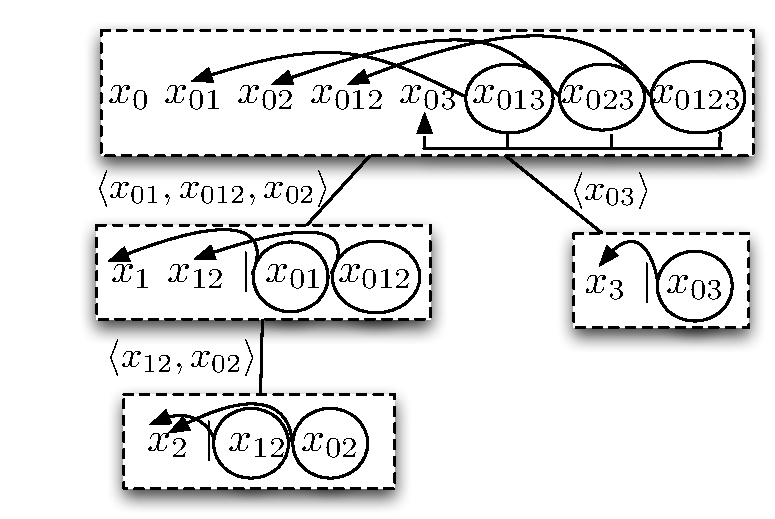
\includegraphics[scale=0.47]{img/clique_representation}
} 
\caption{\label{fig:cycle_graph} Example of (a) a graph with a
cycle ($G$); (b) a pseudotree $PT$ of $G$; and (c) a clique tree of $PT$.}
\end{figure}

\noindent Then, \emph{SCF-Graphs} runs into three
phases:
\begin{itemize}
\item \textit{Demand propagation} phase
\item \textit{Main} phase
\item \textit{Offer propagation} phase 
\end{itemize}

\noindent during which agents exchange two kinds of messages:
(i) \textit{demand messages}, to exchange demands through tree-edges for
requiring coalitions whose activation is required by some agent up to $PT$;
and (ii) \textit{offer messages}, to propagate offers through tree- and pseudo-
edges for required coalitions to agents down $PT$.

\noindent In what follows we describe the main phases of the $\emph{SCF-Graphs}$
algorithm using the trace in Figure \ref{fig:execution} of an execution of
$\emph{SCF-Graphs}$ over the the pseudotree arrangement of the $CG$ cyclic graph
game in Figure \ref{fig:cycle_graph_a}.
%Demand messages are exchanged up the tree through tree-edges. In contrast,
% offer messages are exchanged down the tree through tree and pseudo-edges.

\begin{figure}[!ht]
\subfigure[]{
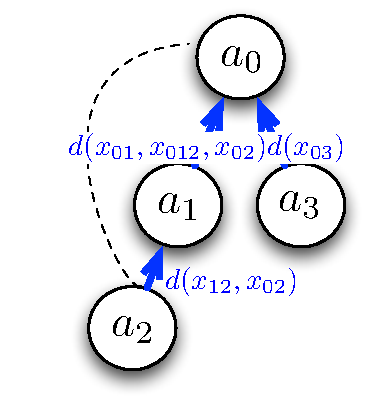
\includegraphics[scale=0.46]{img/step1}
}
\subfigure[]{
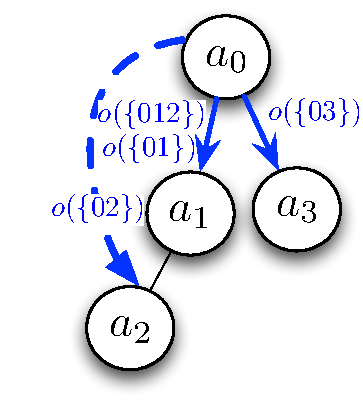
\includegraphics[scale=0.46]{img/step2}
}
\subfigure[]{
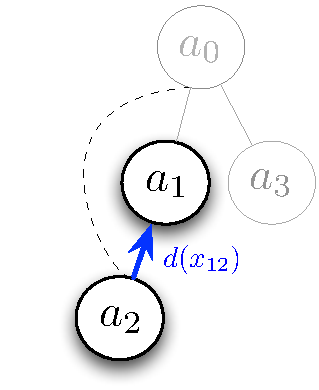
\includegraphics[scale=0.46]{img/step3}
}
\subfigure[]{
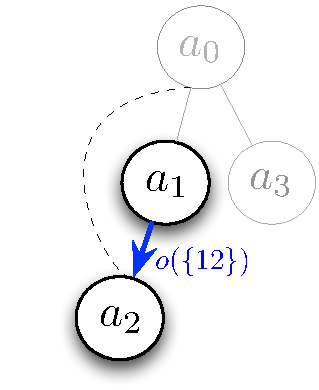
\includegraphics[scale=0.46]{img/step4}
}
\caption{\label{fig:execution} Messages exchanged at different steps of the
execution of \emph{SCF-Graphs} over the clique tree in Figure
\ref{fig:cycle_graph}.}
\end{figure}

\noindent Each agent $a_i$ starts the \textit{demand propagation phase} waiting until
receiving a \emph{demand} message from each of its children $a_j\in Ch_i$ (line
3).
%Thus, independently of the graph at the beginning of the algorithm agents
%propagate demand messages through all edges up the $PT$. 
Figure \ref{fig:execution}(a) depicts the demand messages exchanged during this
phase. Thus, agent $a_1$ waits until it receives the \emph{demand}
message from $a_2$ that contains a function over feasible configurations of 
variables $X_{21}=\{x_{12},x_{02}\}$ before computing the demand message for
its parent $a_0$. To compute its demand for its parent, each agent needs first
to compute its \textit{payment function} and its \textit{expected payment}
(Procedure \texttt{demand\_propagation}).
Each agent $a_i$ computes its payment function, $P_i(X^{P}_{i})$, as
the combination of its value function, $V_i(X_i)$, and the (last)
\emph{demand} messages from its children that subtract the amount required for agents down $a_i$.

Thus, in Figure \ref{fig:execution}(a), agent $a_1$ will combine its value
function $V_1(X_{1})$ with the demand received from $a_2$.
Notice that the payment function depends on a set of variables $X^{P}_{i}$, that
is the set of variables of $a_i$ ($X_i$) and the set of variables in the scope
of any demand received from a child $a_j\in Ch_i$ ($X_{ji}$). 
Thus, in
Figure \ref{fig:execution}(a), the payment function of $a_1$ will depend not
only on its variables $X_1$ but also on
some alien coalition variable, namely $x_{02}$, that is propagated from
$a_2$. Then,
$a_i$ computes its expected payment $\rho_i$ as the highest payment he can
get on any of its leading coalitions, that is for any configuration
of a variable in $X^{L}_i$. Thus, in Figure
\ref{fig:execution}(a), $a_1$ computes the highest payment he gets among
variables $x_{1}$,$x_{12}$.
After that, if agent $a_i$ is not the root, $a_i$ sends a message to
its parent $a_p$ that summarizes its payment function $P_i$ over all possible
configurations of variables in $X_{ji}$ (filtering out its leading variables
$X^{L}_{i}$) and subtracts its expected payment $\rho_i$.
% When summarizing its payment function the agent computes
%its expected payment for each of the alien configurations, that is the best
% payment we can get from its local coalition variables under each of these configurations.
Thus, in Figure \ref{fig:execution}(a), $a_1$ summarizes its payment function
$P_1$ over variables $\{x_{01},x_{012},x_{02}\}$ (filtering out its leading
variables $X^{L}_{1}=\{x_1,x_{12}\}$). 
The result of this summarization is, for each coalition variable $x_S$ in
$X_{ip}$, the demand that agent $a_j$ will need to satisfy to agents in
$A(PT_i)$ to ensure their participation in $S$.

\newpage\noindent In case of an alien variable $x_S\not\in X_i$, this payment is not simply the
amount demand by agents down $PT_i$ but considers the potential loss of $a_i$
when restricting to coalitions that does not contain any agent in $S$ (the
maximum offer $a_i$ is going to offer to agents in $S$ to join).
%itself to coalitions that does not include any agent in $S$.
Thus, in Figure \ref{fig:execution}(a), the demand of agent $a_1$ to its parent
$a_0$ for $x_{02}$ is the maximum between the amount demanded from $a_2$ to join
this coalition and the potential loss of $a_1$ from moving to a coalition
($\{1\}$) that does not include $a_2$.
%These gives as a result four
%configurations $(x_{01}=0,x_{012}=0,x_{02}=0)$,
% $(x_{01}=0,x_{012}=0,x_{02}=1)$, $(x_{01}=0,x_{012}=1,x_{02}=0)$, $(x_{01}=1,x_{012}=0,x_{02}=0)$,
% $(x_{01}=1,x_{012}=0,x_{02}=1)$. 
% Notice that for the configuration
% $(x_{01}=0,x_{012}=0,x_{02}=1)$, agent $a_1$ has computed the best payment
 % from its local variable configurations $x_{1},x_{12}$ compatible with the activation
% of $x_{02}$. Since by the message received for $a_2$, $x_{12}$ can not be
% activated with $x_{02}$, the best payment $a_1$ can get when $x_{02}$ is
% activated is those coming from the composition of coalition $x_{1}$. Then
 % since the expected payment substracted is the best payment $a_i$ can get on
 % any of
% its local coalitions, that includes $x_{1}$ and $x_{12}$. So, the value of the
% demand  $(x_{01}=0,x_{012}=0,x_{02}=1)$ is not simply the amount demanded for
% $a_2$ to join coalition $x_{02}$, but it is the that is the amount $a_1$ is
% loosing from moving to a coalition that does not include $a_2$, that is
% $\{1\}$, and thus the maximum amount he is going to offer to $a_2$ to join.
 %We can get $x_{12},x_{02}$ has three valid configurations $x_{12}=0,x_{02}=0$,
 %$x_{12}=1,x_{02}=0$, $x_{12}=0,x_{02}=1$.
%Example.

%This phase is called demand propagation and it sends the demands of agents up
% to the tree.
Once the \emph{demand propagation} phase is over, agents start the \emph{main
phase} (lines 5-10) in which each agent $a_i$ iteratively checks (line 5):
($C_1$) if he has received an offer for all requiring coalitions ($X^{L}_i\neq
X_i$); and ($C_2$) if its payment depends on some alien coalition, ($X^{P}_i\neq
X_i$).
If any of these two conditions is not satisfied, it means that agents needs to
either receive new demands from children (that get rid of alien variables) or
offers from their ancestors (that make an offer for some requiring
coalition), so agent $a_i$ waits for messages. 
Thus, in Figure \ref{fig:execution}(a)-(d), after the initial demand propagation
phase, agent $a_3$ waits until receiving an offer message from its parent
$a_0$, whereas agent $a_1$ needs to wait for a message from its parent $a_0$ and
a new demand from its child $a_2$ that gets rid of the alien coalition $x_{02}$.
%Notice that for tree
%interaction graphs condition (i) is always satisfied (no alien coalitions are
%propagated in $PT$) and condition (ii) is satisfied as soon as $a_i$ gets an
%offer messages from its parent (its only ancestor in PT). Thus, in acyclic
%interaction graphs, each agent only iterate through the main phase once to wait
%for the offer message from its parent.
When agent $a_i$ receives an offer message over a coalition
$S$, he adds requiring variable $x_S$ to its set of leading variables $X^{L}_i$
(given the offer, now $a_i$ is the leader of coalition $S$) and updates its
value function and optimal decision over $S$.
%Finally, $a_i$ adds the decision of $a_j$ to form or not coalition $S$ in its
% set of optimal configurations, $x^{*}_i \cup (x_S= x^*_S)$  
Additionally, $a_i$ checks if the offer messages comes from its parent in
the pseudotree, in which case the agent marks itself as the new root.
%If it is the case, it means that its parent already decided about which
% coalition to form and computed its payment on it, so the agent mark himself as the new root to avoid send any new demand to its parent when.
%An offer message $o_{j\rightarrow i}(\mathbf{S})$. 
%For each offered requiring
%coalition $S\in \mathbf{S}$, the message contains the value that $a_j$ offers
% to $a_i$ in order to get agents in $S$ ($o(S)$) to join the coalition and the
%decision of $a_j$ to form or not that coalition ($x^*_S$). 
Finally, independently if a new offer or demand is received the
agent re-runs the demand\_propagation procedure recomputing its payment
function, its payment and the demand for its parent.
When $C_1 \wedge C_2$ is satisfied (notice that for the root they are always
satisfied), each agent $a_i$ starts the \textit{offer propagation phase} (lines
9-39). 
%in which computes its optimal configuration and final payment and
%sends offer messages for each requiring coalition down the tree (lines 20-40).
For example, in Figure \ref{fig:execution}, $a_0$, as root, starts the offer
propagation phase just after the initial demand propagation phase.
First, each agent $a_i$ computes its
optimal local configuration $x^*_i$ given the already inferred decision
of its ancestors $An_i$ over requiring coalitions (line 9) and retrieves the
optimal coalition $S^*_i$ corresponding to this optimal configuration (line 10). 
%In Figure \ref{fig:execution}, since $a_0$ has no ancestor, the set of optimal
%configurations $\mathbf{x^*_0}$ stand for the leading coalition configuration
%that maximises its payment. 
%In general, if some ancestor $An_i$ decided to
%create a coalition $S$, and thus is willing to pay the amount requested by
% $a_i$ and other agents agents in $S$ to join, then the best configuration for
%$a_i$ is $\mathbf{x^*_i}=\mathbf{x_S}$.
% Otherwise, $a_i$ selects the optimal
%configuration of the agent would be to activate the required coalition
% $Req_i(S)$.
% Otherwise, $a_i$ selects among its leading coalitions $S\in
%\mathbf{L}_i$ the configuration $\mathbf{x_S}$ that maximises its payment.
Next, each agent locally checks for the emptiness of the core (lines 11-12). The
core is detected as empty if $a_i$ detects that its payment conditioned to the
decision of ancestors ($P_i(x^*_i)$) is less than the best payment he can get
considering all its local configurations ($\rho_i$).
Finally, each agent $a_i$ can start computing the offers of coalitions
requiring some agent down the tree.
%its expected payment
%$\rho_i$ computed as the best payment he can get in any of its local
% configurations (that includes offers from ancestors and values for leading coalitions).
For each of its leading coalitions $S\in L_i$, the offer of agent $a_i$
for $S$ is distributed among
independent offers for $S$'s required coalitions ($Req_i(S)$).
%makes an offer to each required coalition of $S$ to ensure their activation.
 %The offer agent $a_i$ can make to agents
%down the tree $S$ to join him is the payment he gets for $x_S$ but cancelling
%the demands of agents,  minus its payment $\rho_i$.
%The offer should be distributed among offers
%through requiring variables for which it requires the activation. 
%Thus, in Figure \ref{fig:execution}(b), $a_0$ for its local basic coalition
%$\{01\}$ generates an offer for variable $x_{01}$ whereas for its composite
%coalition $\{0,1,3\}$ generates two offers, one for required coalition, that is
%for $x_{01}$ and $x_{03}$.
%Notice that the payment function considers the value the agent can get for this
%coalition (indirectly by an offer or directly as a principal) substracting the
%demands of all required agents down the tree. Then we substract the joint
% demand for variable and not offered demands minus the demands (what we still need to
%offer to variables still not offered).
Each agent $a_i$ computes the offer of a coalition $S$ for a
required coalition $S'$ as the value of its payment function for $S$
minus the $a_i's$ payment (notice that this includes demands from all agents)
canceling the difference between the joint demand for $x_{S'}$ and coalitions
still not offered ($x_{S'\cap o}$) and the joint demand of coalitions
still not offered ($x_{o}$).

\noindent Thus, in Figure \ref{fig:execution}(b), $a_0$ computes the offer of $\{0,1\}$
for $\{0,1\}$ (the only requiring coalition of $\{0,1\}$ in $X_1$ is
itself) as the value of its payment function for $\{0,1\}$ ($P_0(x_{01})$)
minus its payment ($\rho_0$) whereas subtracting the demand from coalition
$\{0,1\}$. Notice that whenever $S$ is a basic coalition the amount offered
to $S$ is just the value of agent $a_i$ for $S$ minus $a_i$'s payment.
% to offer this is the payment
%substracting all the demand cancelling the demand for this coalition itself.
In contrast, when the coalition is composite the offer is distributed among more
than one required coalitions. For example, in Figure \ref{fig:execution}(b), the
offer of $a_0$ for its leading coalition $\{0,1,3\}$ is distributed among its
requiring coalitions $\{0,1\}$ and $\{0,3\}$.
% Thus, $a_0$ computes the offer of
%$\{013\}$ for $\{01\}$ as the value of its payment function for $\{013\}$
%($P_0(\mathbf{x_{013}})$) minus its payment ($\rho_0$) cancelling the
% difference between the joint demand for $x_{01},x_{03}$ and the demands for $x_{03}$
%alone.
%This is
%done in that way because if there is an extra demand to activate
% $x_{01},x_{03}$ together with respect the individual demands of $x_{01}$ and $x_{03}$
%($d(x_{01}=1,x_{03}=1)> d(x_{01}=1) + d(x_{03}=1)$) this is included in the
%offer for $x_{01}$ (to be preceding in the ordering).
 %Thus, in Figure \ref{fig:execution}(b), for
%coalition $x_{03}$ is the payment for $\{0,1,3\}$ minus the payment of $\rho_0$
%cancelling the difference between the demands to activate $x_{03}$.
%Agent $a_i$ would update only the value of the offer for some basic coalition
%iff it improves the current offer. For example, in Figure , the offer computed
%by $a_0$ for its basic coalition $x_{01}$ is the best offer between those
% coming for coalition $\{0,1\}$ and those coming for coalition $\{0,1,3\}$.
After computing offers, each agent $a_i$ sends for each of its basic coalitions
$\{S \in L_i \vert Req_i(S)=\{S\}\}$, an offer message to the agent in
$S\setminus\{i\}$ with higher position in $PT$  (lines
36-39).
%Thus, in Figure \ref{fig:execution}(b) $a_0$ sends offer messages to each
%descendant, namely to $a_1$, $a_2$ and $a_3$ with offers for the respective
% requiring coalitions namely $\{\{01\},\{012\}\}$, $\{\{02\}\}$, $\{\{03\}\}$.
At the end of the algorithm (line 41), agents run a distributed
procedure\footnote{Any distributed algorithm used for convergence detection can be used for that purpose.} to
propagate the core status across the graph (emptiness of the core is propagated through the whole
graph). 

\noindent In this way, \textit{SCF-Graphs} builds an optimal and stable solution, if one exists, otherwise the emptiness of the core is detected and propagated among all agents, as stated by Theorem \ref{th:scfcorrect}.
 
\begin{Th}\label{th:scfcorrect}
Given a game on a graph $CG=\langle A(G), v, F(G)\rangle$, if the core of $CG$ is not empty, the outcome produced by SCF-Graphs belongs to the core of $CG$; otherwise SCF-Graphs outcomes the optimal coalition structure of $CG$ detecting the emptiness of the core.
\end{Th}

\begin{algorithm}
\caption{SCF-Graphs}
\label{algo:scfgraphs}
\small Each $a_i$ knows $\langle a_p,  X_i,\psi_i(X_{\psi_i}),Req\_i,\rho_{min}\rangle$ 
\begin{algorithmic}[1]
\State $\texttt{EMPTY\_CORE}_i\gets false$
\State $\forall{x_S \in X_{\psi_i}}: o(x_S)\gets 0$ 
\State Wait for a demand message from each child $a_j\in Ch_i$ ($d_{j \rightarrow i}(Sep_{ji})$)
\State $\langle p_i(X_{C_i}), \rho_i \rangle \gets \texttt{demand\_propagation()}$
\While{$X_{C_i}\neq X_{\psi_i} \vee X_{i}\neq X_{\psi_i}$}
\State \texttt{handle\_messages()} 
\State $\langle p_i(X_{C_i}), \rho_i \rangle \gets \texttt{demand\_propagation()}$
\EndWhile
\State $X^*_{i} = \operatorname*{arg\,max}_{X_{i}, X^{*}_i} p_i(X_{i})$
\State $S^*_i=\gamma(X^*_{i})$
\If{$p_i(X^*_{i})\neq \rho_i$}
\State $\texttt{EMPTY\_CORE}_i=true$
\EndIf  
\ForAll{$x_S \in X_i$}
\If{$Req_i(x_S) = \emptyset$}
\State $\texttt{OFFER}_i \gets p_i(x_S=1,X_{i}=0) -\rho_i-\sum_{j\in Ch_i} d_{j\rightarrow i}(x_S=1, X_{i}=0)$
\If{$S^*_i=S$}
\State $\texttt{OFFER}_i \gets \texttt{OFFER}_i + \rho_{min}\cdot \vert S\setminus \{a_i\}\vert $
\EndIf 
\State $o(x_{S})\gets max(o(x_{S}),\texttt{OFFER}_i)$
\Else
\State $X_{\setminus o} \gets Req_i(x_S)$
\ForAll{$x_{S'} \in Req_i(x_S)$} 
\State $X_{\setminus o} \gets X_{\setminus o} \setminus \{x_{S'}\} $
\State $\texttt{h}_i=\sum_{j\in Ch_i} d_{j\rightarrow i}(x_S=1, x_{S'}=1, X_{\setminus o} = 1,X_{i}=0)$
\State $\texttt{k}_i=\sum_{j\in Ch_i}d_{j\rightarrow i}(x_S=0, x_{S'}=0, X_{\setminus o} = 1,X_{i}=0)$
\State $\texttt{OFFER}_i \gets p_i(x_S=1,Req_i(x_S)=1,X_{i}=0)-\rho_i-\texttt{h}_i +\texttt{k}_i$
\If{$S^*_i=S$}
\State $\texttt{OFFER}_i \gets \texttt{OFFER}_i + \rho_{min}\cdot \vert S'\setminus \{a_i\}\vert $
\EndIf 
\State $o(x_{S'})\gets max(o(x_{S'}),\texttt{OFFER}_i)$
\EndFor
\EndIf
\EndFor
\State $\rho_i \gets  \rho_i - \rho_{min}\cdot \vert S^*_i\setminus \{a_i\}\vert$
\ForAll{$x_{S} \in X_i \vert Req_i(x_S)=\emptyset $ }
\State Let $a_j$ be the agent in $S\setminus \{a_i\}$ with highest level
\State $o_{i\rightarrow j}\gets o_{i\rightarrow j} \cup \langle x_{S}, o(x_{S}=1),x^*_{S}\rangle$
\EndFor
\State Send $\texttt{OFFER}_i$ messages to respective agents
\State $\texttt{EMPTY\_CORE}_i\gets \texttt{propagate\_core\_status(EMPTY\_CORE}_i\texttt{)}$
\If{$\texttt{EMPTY\_CORE}_i = true$}
\State $\rho_i \gets \infty$
\EndIf
\end{algorithmic}
\label{proc:scf_graphs}
\end{algorithm}
 
\begin{algorithm}[!tb]
\caption{\texttt{handle\_messages	}} 
\begin{algorithmic}
\State \texttt{Wait\_for\_messages()}
\ForAll{For each message received}
\If{offer $o_{j \rightarrow i}(Sep_{ji})$ message received}
\If{$a_j=a_p$}
\State $a_i \gets root$
\EndIf
\ForAll{$\langle x_S, o(x_S) , x^*_S \rangle \in o_{j \rightarrow i}$}
\State $X_i \leftarrow X_i \cup x_S$
\State $o(x_S=1)\leftarrow o(x_S)$ 
\State $X^{*}_i \leftarrow X^{*}_i \cup (x_S=x^*_S)$ 
\EndFor
\EndIf
\EndFor
\end{algorithmic}
\end{algorithm}

\begin{algorithm}[!tb]
\caption{\texttt{propagate\_core\_status}} 
\begin{algorithmic}
\State Wait from $\texttt{EMPTY\_CORE}_j$ from each child $a_j\in Ch_i$
\If{$\exists k : \texttt{EMPTY\_CORE}_k = true$} 
\State $\texttt{EMPTY\_CORE}_i=true$
\EndIf
\If{$a_i\neq root$}
\State Send $\texttt{EMPTY\_CORE}_i$ to $a_p$
\State Wait from message from $a_p$
\State $\texttt{EMPTY\_CORE}_i\gets\texttt{EMPTY\_CORE}_p$
\EndIf
\State Send $\texttt{EMPTY\_CORE}_i$ to all children $Ch_i$
\end{algorithmic}
\end{algorithm}

\begin{algorithm}[!tb]
\caption{\texttt{demand\_propagation}} 
\begin{algorithmic}
\State $p_i(X_{C_i}) = \psi_i(X_{\psi_i}) \otimes \bigotimes_{j \in Ch_i} d_{j \rightarrow i}(Sep_{ji})\otimes \bigotimes_{x_S \in X^{\setminus r}_i}o(x_S)$ 
\State $\rho_i = \max_{X_{i}} p_i(X_{i})$
\If{$a_i\neq root$}
\State $d_{i \rightarrow p}(Sep_{ip})= \max_{X_i} p_i(X_{C_i}) - \rho_i$ 
\State Send $d_{i\rightarrow p}(Sep_{ip})$ to $a_p$
\EndIf
\end{algorithmic}
\end{algorithm}

%%%%%%%%%%%%%%%%%%%%%%%%%%%%%%%%%%%%%%%%%%%%%%%%%%%%%%%%%%%%%%%%%%%%%%%%%%%%%%%%%%%%%%%%%%%%%%%%%%%%%%%%%%%%%%%%
%% Chapter %%%%%%%%%%%%%%%%%%%%%%%%%%%%%%%%%%%%%%%%%%%%%%%%%%%%%%%%%%%%%%%%%%%%%%%%%%%%%%%%%%%%%%%%%%%%%%%%%%%%%
%%%%%%%%%%%%%%%%%%%%%%%%%%%%%%%%%%%%%%%%%%%%%%%%%%%%%%%%%%%%%%%%%%%%%%%%%%%%%%%%%%%%%%%%%%%%%%%%%%%%%%%%%%%%%%%%

\chapter{Application to the Energy Market}\label{chap:energy}

In this chapter we will show how the aforementioned theoretical notions and solution techniques -- especially the GDL-based message-passing algorithm -- can be applied to a real-world case study: the energy market. We will focus on a scenario in which a group of energy customers have a demand of energy supplies (\textit{e.g.} electrical power), and need to buy them in a way that minimizes their costs, forming \textit{coalitions}.
We assume that energy customers are organized in a social network. The social network models the knowledge relationships between energy customers and restricts the structure of possible coalitions they can form. This network can be trivially represented by a graph with certain particular properties, formally discussed in Section \ref{sec:socnet}.

It is easy to see that this setting has a natural modelization in \textit{coalitional games on graphs} defined in Section \ref{subsec:coalgamesgraph}, in which players are considered to be \textit{selfish}, thus setting us in a non-cooperative environment. As said before, real energy customers have little interest in increasing system gain, as their main concern is to maximize their own utility, with the simple goal of having a cheaper bill. Therefore, the concept of \textit{stability} introduced in Section \ref{subsec:core} assumes a key role, since it is not possible to impose a solution ``from above'', as it would be immediately rejected by the agents. 
Rather, the goal is to find an appropriate distribution of payments that incentives single energy customers to maintain the current structure, as any deviation would worsen their payoff, making energy more expensive.

\section{The Problem}

In all current electricity grids this balance is
achieved by varying the supply-side to continuously match demand.
The amount of demand required on a continuous basis is usually carried by the
baseload stations owing to low cost generation, efficiency and safety.

\noindent However, these stations are slow to fire up and cool down, so they are not able to match
the peakload periods that exceed this baseload that
require, in contrast, the use of expensive, carbon-intensive, peaking plant generators.
Although only running when there is high demand, these peaking plant generators are responsible of most part of consumers
electricity bill.

Along this line, the vision of the \textit{smart grid} includes demand-side peak-shaving
strategies such as real-time pricing or profile's based tariffs to encourage
consumption such that the peaks on demand are \emph{flattened}
\cite{GridVision}. A flattered demand results in a more efficient grid not only
with lower carbon emissions but also with lower prices for
consumers. Hence, some works \cite{DBLP:conf/atal/RamchurnVRJ11,
DBLP:journals/network/TomprosMDFH09} focused on techniques that flatten
individual consumer demand by automatically controlling home domestic or micro-storage devices. Unluckily,
since each consumer independently optimizes its own consumption,
the effectiveness of this approach has a clear limit on the consumer's restrictions
and comfort (\textit{e.g.} it will be unavoidable to get a consumption peak in the
non-working hours of consumers).

Against this background, the problem of how the grid efficiency can be
further improved from a social perspective is investigated. In particular, we explore the
idea of allowing consumers to join into coalitions with other consumers with
complementary energy needs. Then, a group of consumers can act in the market
as a single virtual consumer with a flattened demand for which it gets much better
prices. As part of the smart grid community, electricity consumers have already
access to smart meters that allow them to monitor its (load) energy profile\footnote{
The load energy profile is a graph of the variation in the electrical load versus
time.} in an hour-day basis (Figure \ref{fig:energyprofile}). Thus, the energy profile of a customer $a_i$ can be represented as a vector $E_i=\{e^1_i,\ldots,e^T_i\}$ where $e^t_i$ is the amount of energy consumed at time slot $t$ and $T$ is the length of the considered interval.

\begin{figure}[!h]
	\centering
	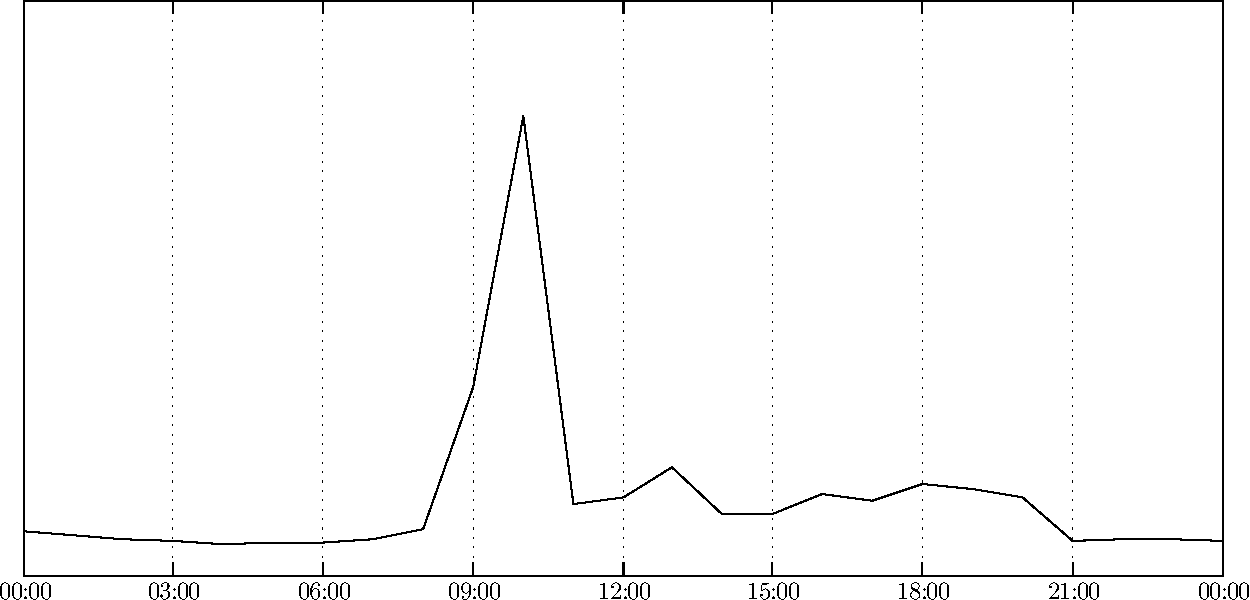
\includegraphics[width=0.95\textwidth]{img/energy_profile.pdf}
	\caption{\label{fig:energyprofile}Typical energetic profile over 24 hours}
\end{figure}

\section{Social networks}\label{sec:socnet}

Given the huge recent success of social networks (\textit{e.g.} at the time of writing Facebook has more
than 500 millions users), consumers can use them as free interaction tools to self-organize into energy coalitions.

Social networks not only provide a way of interaction
among energy consumers but also restrict coalition membership by reflecting
realistic barriers to the formation of certain coalitions. In
particular, consumers may not want to join coalitions with unknown consumers for
which they do not have any source of trust regarding their reported profiles or
their capacity to meet their payment obligations. In contrast, if the social
network is used to restrict coalition membership, customers join
coalitions of \emph{friends of friends}, thus being sure that someone they know directly is always involved.

Social networks have been used in many different fields of study, such as biology, communication studies, economics, information science, organizational studies, and sociology. Given this wide variety of topics and formalization, we will focus only on two categories of social networks, which have been deeply studied and can be modeled through mathematical procedures: \textit{scale-free networks} and \textit{small-world networks}\footnote{In the experimental cases, these topologies will the tested against \textit{random networks}, which will be used as a benchmark}.

\subsection{Scale-free networks}

\begin{Def}[Scale-free network]
A \textit{scale-free network} is a network in which the degree distribution follows a power law, at least asymptotically. That is, the fraction $P(k)$ of nodes in the network having $k$ connections to other nodes goes for large values of $k$ as:
$$P\left(k\right) \sim ck^{-\gamma}$$
where $c$ is a normalization constant and $\gamma$ is a parameter whose value is typically in the range $2 < \gamma < 3$, although it may lie outside these bounds.
\end{Def}

\noindent Scale-free networks are believed to be the model of many real-world networks, including World Wide Web links, biological networks, and social networks, although the scientific community is still discussing these claims as more sophisticated data analysis techniques become available \cite{Clauset:SIAM2007}. 

Many models have been proposed as mechanisms to explain conjectured power law degree distributions in real networks, such as \textit{preferential attachment}, which refers to the process according to which the likelihood of connecting to a node depends on the node’s degree. For example, a web page will more likely include hyperlinks to popular documents with already high degrees, because such highly connected documents are easy to find and thus well known.

\noindent This mechanism is the base of the model proposed by Barabàsi and Albert \cite{2002RvMP...74...47A}, who studied the growth of social network and provided a simple algorithm to generate one that follows the properties of scale-free networks.
Starting from a network of $m_0$ initial and connected\footnote{If a node is not connected, it will always remain disconnected from the rest of the network. For example the initial network could be a tree of $m_0$ nodes.} nodes, with $m_0 \geq 2$, new nodes are added to the network one at a time. Each new node is connected to $m$ existing nodes with a probability that is proportional to the number of links that the existing nodes already have. Formally, the probability $p_i$ that the new node is connected to node $i$ is:
$$p_i = \frac{k_i}{\sum_j k_j}$$
Note that $m$ is a parameter of the generator, which determines the final \textit{density} -- number of edges divided by the number of nodes -- of the graph. In some formulation, \textit{exactly} $m$ edges are added at each step, in which case the density can be computed \textit{a priori}; otherwise, a random number in the set $\{1,\ldots,m\}$ is chosen, making the number of edges in the final graph unpredictable. The resulting network can be shown to be scale-free, with a degree distribution of: 
$$P\left(k\right)\sim k^{-3}$$

\noindent The example network shown in Figure \ref{fig:scalefree} has 20 nodes and has been generated with the Barabàsi-Albert model, adding a maximum of 2 nodes per step.

\begin{figure}[!h]
	\centering
	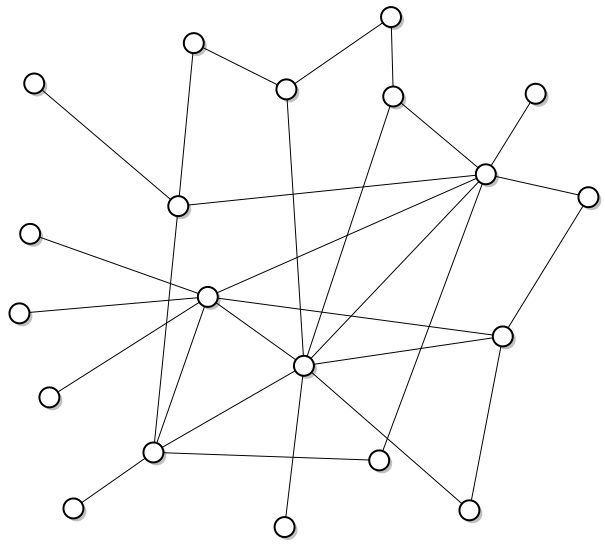
\includegraphics[width=0.66\textwidth]{img/scalefree.png}
	\caption{\label{fig:scalefree}Scale-free network example}
\end{figure}

\subsection{Small-world networks}

An alternative model to characterize social network is provided by \textit{small-world networks}, whose topology is formed in a way such that most of the nodes are not neighbors of one another, but most of them can be reached from every other by a small number of hops or steps.

\begin{Def}[Small-world network]
A \textit{small-world network} is a network where the typical distance $L$ between two randomly chosen nodes (the number of steps required) grows proportionally to the logarithm of the number of nodes $N$ in the network, that is:
$$L \propto \log N$$
\end{Def}

\noindent In the context of social interactions, the formation of small-world networks is the result of strangers being linked by a mutual acquaintance. Many empirical graphs are well-modeled by small-world networks. Social networks, wikis\footnote{A \textit{wiki} is a website whose users can add, modify, or delete its content via a web browser using a simplified markup language or a rich-text editor.} such as Wikipedia, and gene networks all exhibit small-world characteristics.

This kind of networks were deeply studied by Watts and Strogatz \cite{citeulike:99}, who identified two structural parameters used to classify the features of a particular network, namely the \textit{clustering coefficient}, a measure of degree to which nodes tend to cluster together, and the \textit{average shortest path length}. They also noticed that in purely random graphs build with the Erdős-Rényi model \cite{Erdos1959}, both these parameters are low, while the clustering coefficient measured in many real-world networks significantly higher than expected, maintaining a small average shortest path length.

These are the main features enforced by the Watts-Strogatz model: Figure \ref{fig:smallworld} shows an example of a small-world network of 20 nodes generated with this algorithm. 

The typical ring-like structure is the consequence of the initial ring lattice of $n$ nodes, connected to $k$ other ones ($\frac{k}{2}$ per side, imposing that $k$ must be even), which is subject to a \textit{rewiring} process, which replaces some edges with a probability given by the parameter $\beta$.

The aforementioned properties make cliques, and near-cliques, very likely to form in this type of graphs. In addition to this, there are several other features that small-world networks tend to have: typically, there is an over-abundance of \textit{hubs} -- nodes in the network with a high number of connections (known as high degree). These hubs serve as the common connections mediating the short path lengths between other edges. By analogy, the small-world network of airline flights has a small mean-path length (\textit{i.e.} between any two cities you are likely to have to take three or fewer flights) because many flights are routed through hub cities.

\begin{figure}[!h]
	\centering
	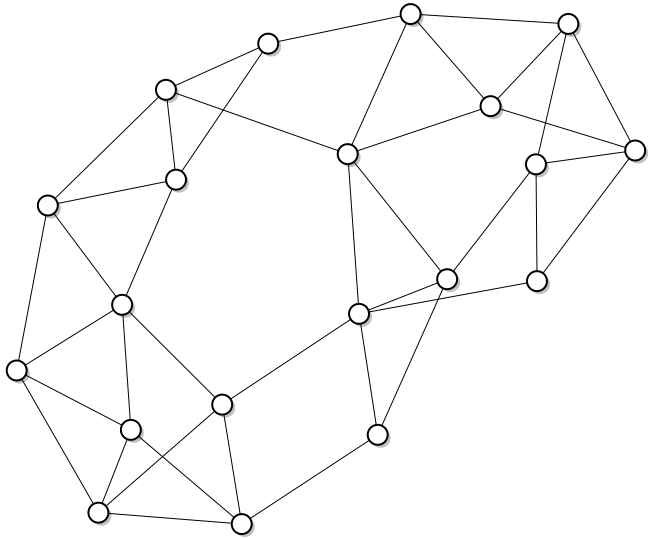
\includegraphics[width=0.7\textwidth]{img/smallworld.png}
	\caption{\label{fig:smallworld}Small-world network example}
\end{figure}

\section{Buying in the Energy Market}

In economic terms, electricity is a \textit{commodity}\footnote{From the economic point of view, a \textit{commodity} is the generic term for any marketable item produced to satisfy wants or needs.} capable of being bought, sold and traded. Thus, we refer as \textit{energy market} as the system that allows to buy (through bids), sell and make short-term trades related to energy, generally in the form of financial or obligation swaps. Bids and offers use supply and demand principles to set the price. Long-term trades are contracts similar to power purchase agreements and generally considered private bi-lateral transactions between counterparties.
Wholesale transactions (bids and offers) in electricity are typically cleared and settled by the market operator or a special-purpose independent entity charged exclusively with that function. Market operators do not clear trades but often require knowledge of the trade in order to maintain generation and load balance.

Electricity is by its nature difficult to store and has to be available on demand. Consequently, unlike other products, it is not possible, under normal operating conditions, to keep it in stock, ration it or have customers queue for it. Furthermore, demand and supply vary continuously.

There is therefore a physical requirement for a controlling agency, the \textit{transmission system operator}, to coordinate the dispatch of generating units to meet the expected demand of the system across the transmission grid. If there is a mismatch between supply and demand the generators speed up or slow down causing the system frequency (either 50 or 60 hertz) to increase or decrease. 

\noindent If the frequency falls outside a predetermined range the system operator will act to add or remove either generation or load.
In addition, the laws of physics determine how electricity flows through an electricity network. Hence the extent of electricity lost in transmission and the level of congestion on any particular branch of the network will influence the economic dispatch of the generation units.

The scope of each electricity market comprises the transmission grid (or network) that is available to the wholesalers, retailers and the ultimate consumers in any geographic area.

\subsection{Wholesale electricity market}\label{sec:wholesale}

A \textit{wholesale electricity market} exists when competing generators offer their electricity output to retailers. The retailers then re-price the electricity and take it to market. While wholesale pricing used to be the exclusive domain of large retail suppliers, increasingly markets are beginning to open up to end-users. Large end-users seeking to cut out unnecessary overhead in their energy costs are beginning to recognize the advantages inherent in such a purchasing move, moreover, recently consumers have started buying electricity directly from generators too.

Buying wholesale electricity is not without its drawbacks (market uncertainty, membership costs, collateral investment), however, the larger the end user's electrical load, the greater the benefit and incentive to make the switch.
Wholesale markets usually offer two different approaches for the buying strategies users can adopt: a short-term market, where buyers can obtain relatively small quantities of energy, usually intended to be spent in 24 hours, and a long-term market, in which larger amounts of energy can be bought for a longer interval of time. In common terminology, one usually refers respectively to \textit{day-ahead market} and \textit{forward market}.

The system price in the day-ahead market is in principle determined by matching offers from generators to bids from consumers at each node to develop a classic supply and demand equilibrium price, usually on an hourly interval, and is calculated separately for subregions in which the system operator's load flow model indicates that constraints will bind transmission imports.

On the other hand, forward market tends to be more risky, due to an high volatility\footnote{Prices vary significantly over a relatively small period of time} consequence of the complexity of the system, possible peak demand and supply shortage; thus, as a common financial rule, prices are usually cheaper on this market.
Users can access prices in real-time, simply accessing wholesale markets websites \cite{GME}, which offer detailed reports and data regarding the current prices of short and long term market, together with information about purchased volumes of energy (Figure \ref{fig:energy_report}).

\noindent Electricity customers and power producers tend to protect themselves from forward market instability buying energy in an aggregate form, thus forming the appropriate groups -- or \textit{coalitions} -- satisfying everyone's demands is a fundamental task. 

Long-term market offers a wide variety of contracts available to the investors, however the simplest and most commonly used form is represented by \textit{fixed price forward contracts}, in which parts agree to trade a good -- \textit{e.g.} electric energy -- at a specified future time with a price agreed today. Thus, the importance of having a flatter, more predictable usage profile becomes clear, since it allows groups of customers to buy larger stocks at a smaller price, minimizing the wasted amount of energy, which is also important from an ecological point of view.
Thus, for a correct evaluation of a given solution, a precise, formal method that associates a coalition with its quality is needed. We will now introduce some of the metrics defined for this purpose, which have been adopted in the experimental tests.

\begin{figure}[!h]
	\centering
	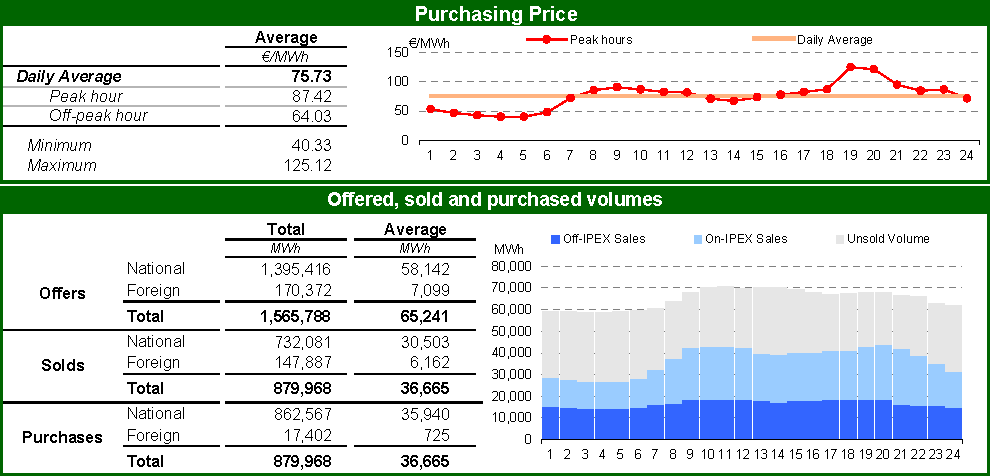
\includegraphics[width=0.79\textwidth]{img/day_ahead.pdf}
	\caption{\label{fig:energy_report}Example of a report with price profile and volume exchange data}
\end{figure}

\section{Metrics}\label{sec:metric}

Another fundamental problem addressed in this thesis is the choice of a appropriate metric to evaluate how the considered coalition is suitable to users' demands. From a formal point of view, the metric simply represents the \textit{characteristic function} of the considered game (as defined in Definition \ref{def:game}). As pointed out before, ``good'' coalition are groups whose joint energy profile\footnote{Analogously to single customer coalitions, we represent the joint energy profile of a coalition $S$ as a vector $E_S=\{e^1_S,\ldots,e^T_S\}$ where $e^t_S=\sum_{i\in S}e^t_i$.} is ``flattened'', because more energy can be bought in a cheaper way on the forward market, so the metrics described hereafter have the primary objective of quantifying this feature, attempting to assign a smaller value to a profile with a peaky behavior, while encouraging the formation of coalitions whose profiles are more regular.

In addition, another eligible property of the metric is non-superadditivity: as described in Section \ref{sec:superaddgames}, in superadditive games the optimal coalition structure is always given by the \textit{grand coalition}. In this context, it would imply putting every agent in the same group, making everyone buying energy together, which is just not reasonable. Furthermore, in real-world environments the complex dynamics and the increased coordination costs of bigger groups make the setting intrinsically non-superadditive.

We will now present some metrics used in the actual implementation of the GDL algorithm presented in Chapter \ref{chap:gdl} and adopted for the empirical test described in Chapter \ref{chap:results}, specifically the \textit{load diversity factor} and the \textit{user price factor}.

\subsection{Load diversity factor}

The first approach used in the definition of a metric is to focus on the ``smoothness'' of the aggregate profile obtained summing the energetic profiles.

The \textit{load diversity factor} of a coalition $S$ $(LDF(S))$ is computed as:
\begin{Def}[Load diversity factor]
\begin{equation}\label{eq:ldf}LDF\left(S\right)=\frac{\sum_{i \in S} {max}_t E_i}{{max}_t E_S} + |S| - 1\end{equation}
where $E_i$ refers to the energy profile of the user $i$ and $E_S$ refers to the joint energy profile of coalition $S$.
\end{Def}

\noindent It is easy to show that the quantity computed by the fractional term is always $\geq 1$; intuitively, if the sum of the peaks of single users (given by the numerator) is close to the maximum of the joint profile, this value is lower, meaning that the maximum values of the individual profiles are positioned at the same time.
Since this is the exact situation we want to avoid, the load diversity factor needs to be maximized, making it suitable for the aforementioned applications.

The additional $|S| - 1$ is due to the fact that, if we only consider the fractional term, the LDF of a single coalition is exactly 1, while, in general, for coalition of $n$ users it is $<n$, making more profitable for players to go always alone.

Since we want to avoid this situation, encouraging the formation of groups, we reward each coalition with an additional value equal to the number of single coalitions avoided. For example, if agent 1 joins agent 2 in the coalition $\{1,2\}$, one single coalition is avoided, \textit{i.e.} an empty coalition must be considered, assumed to have a value of 1. In general, it is easy to see that if a coalition $S$ of $n$ users is formed ($|S|=n$), $n-1$ single coalitions are avoided, increasing the value of $S$ of $|S|-1$.

\noindent From the test performed, load diversity factor allows to form coalition with a good quality for the system, but the value computed has no correlation with the final cost paid by the members of the group. Moreover, the interpretation of the empty coalitions is not clear and cannot be rigorously justified.

For these reasons, a different metric has been developed, the \textit{user price factor}, which effectively captures the monetary gain users can obtain in the formation of coalition to buy from the energy market.

\subsection{User price factor}\label{sec:upf}

The value of a coalition $S$, $v(S)$, is the total payment that the set of
consumers need to carry out to cover the demand of their joint energy profile. As described before, we consider that
customers buy directly their electricity in two different markets: the forward
market and the day-ahead market. In the forward market, consumers in a coalition
$S$ buy in advance the fix continuous amount of energy of their joint
energy profile, $base(S)$, for a better price. The amount of energy that exceeds
this baseload, $peak(S)$, is bought in the day-ahead market.

\begin{Def}[User price factor]\label{def:upf}
The \textit{user price factor} of a coalition $S$ $(UPF(S))$ is computed as:
\begin{equation}\label{eq:upf}UPF\left(S\right)=-base(S) \cdot p_{F} -peak\left(S\right) \cdot p_{DA}-k\left(S\right)\end{equation}
where $p_{F}$ and $p_{DA}$ are the unit energy price in the forward and the day-ahead market
respectively.
\end{Def}

\noindent Since $p_{F}< p_{DA}$, the flattered the energy profile, the most a coalition of consumers can buy in the forward market and the lower the payment of the coalition.
The term $k\left(S\right)$ is intended to represent the negative contributions due to the additional costs necessary to manage a bigger coalition, such as increased coordination costs and more complex dynamics inside the coalition. Thus, $k(S)$ must be proportional to the size of the coalition, and in this work it is assumed $k(S)=(|S| - 1) \cdot\frac{p_{F}}{T}$, where $T$ is the length of the considered time interval. 

From the tests shown in Chapter \ref{chap:results}, user price factor has performed well, allowing the formation of mid-sized coalition, thus avoiding superadditivity. We remark this is simply the result of reasonable considerations, consequence of the real-life behavior of big groups of agents.

It is important to note that Definition \ref{def:upf} does not specify how the actual quantity $base(S)$ is computed, allowing the users to choose from different strategies for the transactions with the forward market. For example, a team could adopt a completely risk-free strategy, buying from the long term market only the quantity of energy it is absolutely sure to consume; in this case, $base(S)=min_t E_S\cdot T$.
\newpage

\noindent Rather, a more risky approach can be used: a coalition might choose to buy more energy from the forward market than the continuous quantity it is sure to consume (represented by the minimum). Thus, a coalition $S$ buys more energy in the forward market but some of this energy is not expected to be consumed. Figure \ref{fig:upf} shows an example of this strategy: the dark amount represents the safer base load, corresponding to the minimum of the profile; then if the light amount is bought, following a more risky approach, more energy will be obtained at a cheaper price, but the marked quantities are not expected to be consumed by the coalition and hence, will be wasted. Although buying more energy than the expected consumption, this strategy can be perfectly rational for agents, in order to get better prices, if the amount of risk taken is directly proportional to the ration between the price of the energy in the forward market and the price in the day-ahead market. Thus, the base load to buy in the forward market to maximize the coalition gain is the maximum amount such that at least the fraction $\frac{p_F}{p_{DA}}$ is expected to be consumed.

\begin{figure}[!h]
	\centering
	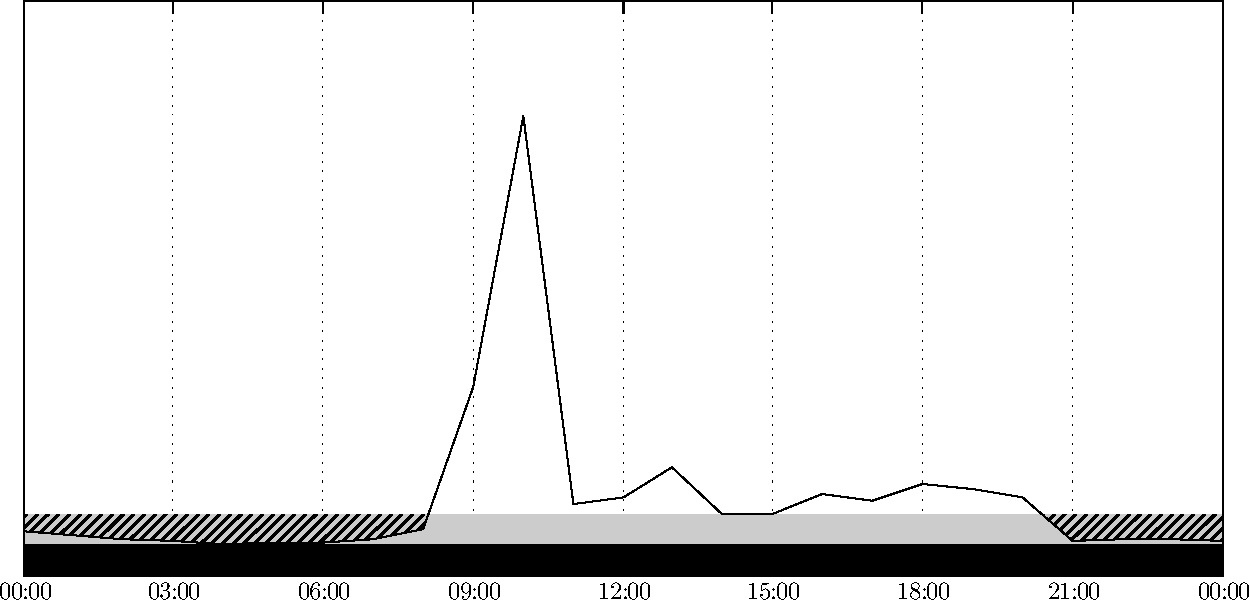
\includegraphics[width=0.95\textwidth]{img/upf.pdf}
	\caption{\label{fig:upf}Example of different base loads for the same energy profile}
\end{figure}

\noindent Algorithm \ref{algo:w} shows how to easily compute this quantity assuming the profile $E$ is discretized in $m$ time parts, thus considering it as an array of $m$ elements. Then, after ordering the $m$ elements in descending order, the base load is the element in position $m \cdot \frac{p_F}{p_{DA}}$, multiplied for the length of the time interval. Coherently, if $p_F = p_{DA}$, then the algorithm returns as baseload the minimum quantity that is expected to be consumed.

\begin{algorithm}[!h]\caption{Computation of a risky baseload}\label{algo:w}
\begin{algorithmic}
\State Sort $E_S$ in descending order
\State $n \gets \lfloor m \cdot \frac{p_F}{p_{DA}}\rfloor$
\State $base(S) \gets E_S^n \cdot m$
\end{algorithmic}
\end{algorithm}

\section{Demonstration Application}\label{sec:demo}

To have an interactive visual tool for coalition formation in the energy market, we developed a platform that allows energy
consumers to organize into stable energy profile coalitions. The demonstration application is written in Java and permits the user to interact with the coalition formation process and have detailed informations about the optimal outcome and the possible gains that can be obtained.

The demonstration starts by asking the user the number of energy consumers for the simulation (Figure \ref{fig:intro}). Moreover, the user can choose between creating the social network randomly, or, alternatively, create a user defined social network from scratch.

\begin{figure}[!h]
	\centering
	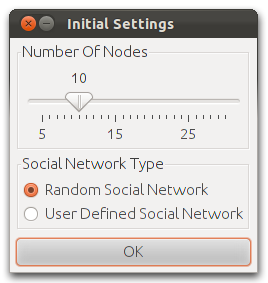
\includegraphics[width=0.49\textwidth]{img/intro.png}
	\caption{\label{fig:intro}Initial dialog of the simulator application}
\end{figure}

\noindent In both cases, the platform generates a set of nodes, one per energy consumer, and allows the user to modify
the network by adding/removing links in an easy way. Each node has an energy profile loaded from real data
characterizing the domestic electricity market and usage patterns of households in the United Kingdom.

Once the coalition formation scenario is set, the simulation starts the \textit{SCF-Graphs} algorithm that organizes energy consumers into stable optimal coalitions. Upon convergence, energy consumers in the same coalition are colored with the same color. For example, observe that in Figure \ref{fig:simulatora}, the coalition $\{0,1,3,4,5,6\}$ was formed, (the grouped agents are all colored in red), whereas consumer 2 is on its own. The interface also highlights the pseudotree used by the algorithm (showing bolded edges) with the associated root node. On the right lower corner, the application also shows the average user gain -- that is the gain that represents the consumer assigned payoff with respect to the value of its individual energy profile.

\begin{figure}[!h]
	\centering
	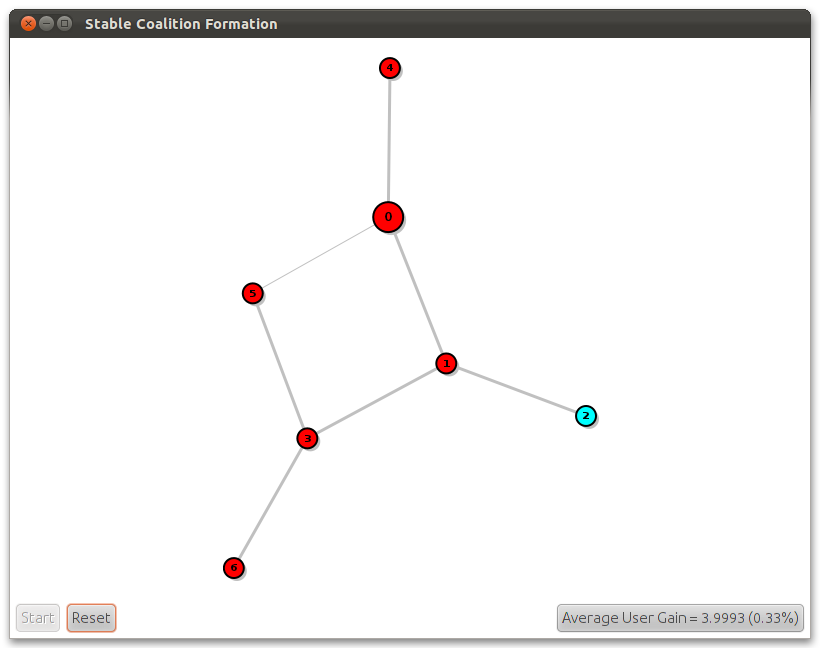
\includegraphics[width=0.78\textwidth]{img/network_coalitions.png}
	\caption{\label{fig:simulatora}The simulator main interface}
\end{figure}

\noindent By clicking on a node, the GUI displays statistical data related to the
specific energy consumer such as its coalition, the coalition's value
and the individual payment that the consumer contributes to the coalition.
%we observe that consumer joins consumer 1,2, and 3 in a joint coalition with a
%total payment of ?. We also observe that this consumer contributes to the
%coalition with an individual payment of ? which represents a gain of 2.
Consumers payments are set in such a way that consumers do not have any
incentive to deviate. 
Finally, the interface also allows to visualize the energetic profiles of coalition members (see Figure \ref{fig:simulatorb}).
Each chart plots a consumer energy profile, delimited by a red line, and the joint coalition energy profile,
delimited by a blue line. The difference between the joint and the individual profile is
filled in the same color used to mark the considered partition (red in the example). 
The GUI offers the user an effective way of restarting simulations after reconfiguring the network
topology, testing how the existence or the nonexistence of a particular link affects the emerging
coalitions and consumers gain.
%  : (i) changing the connections
%among energy consumers; (ii) playing with different topologies

%the
%possibility of rerunning simulations, changing the
%connections among energy consumers, playing with different topologies and
%testing how the existence or the nonexistence of a particular link affects the
%emerging coalitions and consumers gain.

As a simulator, this platform provides to the users with a proof of concept of
what we can do already today as energy consumers in order to get cheaper and
greener energy. Furthermore, it presents the decentralized coalition formation
problem among energy users to the community as an exciting real-world domain for
the applicability of multi-agent technology.
This application has been the subject of a demo paper submitted at \textit{11th International Conference on Autonomous Agents and Multiagent Systems (AAMAS 2012)} \cite{bistaffa} and is available for download as an executable JAR file at \url{http://profs.sci.univr.it/\textasciitilde farinelli/energySCF.jar}. Moreover an illustrative video, describing the simulator and the related topics can be viewed at \url{http://www.youtube.com/watch?v=FT25oETMkfw}.

\begin{figure}[!h]
	\centering
	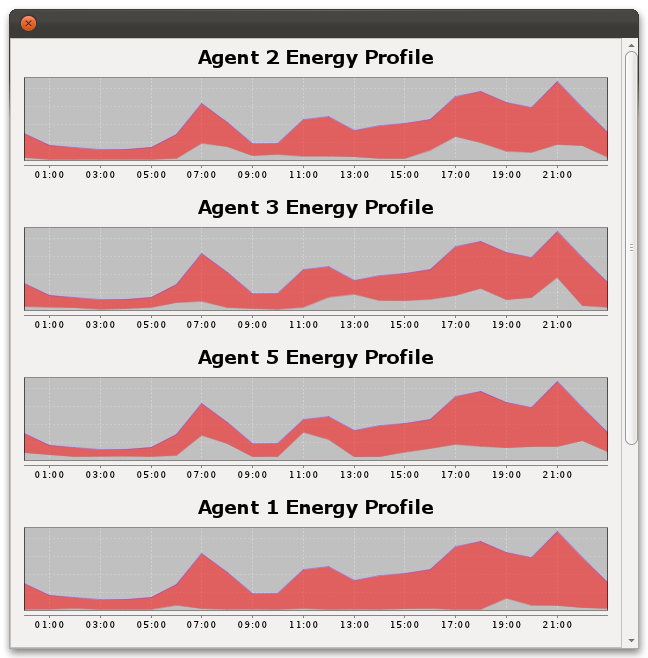
\includegraphics[width=0.9\textwidth]{img/profiles.png}
	\caption{\label{fig:simulatorb}The coalition energy profile inspector}
\end{figure}

%%%%%%%%%%%%%%%%%%%%%%%%%%%%%%%%%%%%%%%%%%%%%%%%%%%%%%%%%%%%%%%%%%%%%%%%%%%%%%%%%%%%%%%%%%%%%%%%%%%%%%%%%%%%%%%%
%% Chapter %%%%%%%%%%%%%%%%%%%%%%%%%%%%%%%%%%%%%%%%%%%%%%%%%%%%%%%%%%%%%%%%%%%%%%%%%%%%%%%%%%%%%%%%%%%%%%%%%%%%%
%%%%%%%%%%%%%%%%%%%%%%%%%%%%%%%%%%%%%%%%%%%%%%%%%%%%%%%%%%%%%%%%%%%%%%%%%%%%%%%%%%%%%%%%%%%%%%%%%%%%%%%%%%%%%%%%

\chapter{Results}\label{chap:results}

In this chapter we will present the results of the empirical experiments conducted to test the quality of the presented coalition formation technique. In particular, two fundamental features of the solutions are addressed: the \textit{average user gain} and the \textit{coalition structure}. Intuitively, \textit{average user gain} refers to the effective gain users have obtained adopting the coalition organization proposed by the given outcome, with respect to a naive solution where only single coalitions are formed.

\begin{Def}[Average user gain]
The \textit{average user gain} of set of agents $A$ with the payoff vector $x$ is computed as:
\begin{equation}\label{eq:aug}
AUG(A,x)=\frac{\sum_{i\in A}(x_i-v(\{i\})}{|A|}
\end{equation}
where $x_i$ refers to the individual payment of agent $i$, and $v(\{i\})$ refers to the value of the coalition with agent $i$ alone. In addition, the \textit{average percent user gain} refers to the percentual gain obtained by users w.r.t. the average value of single coalitions $(APUG(A,x)=\frac{AUG(A,x)\cdot |A|}{\sum_{i\in A}v(\{i\})}\cdot 100)$.
\end{Def}

\noindent On the other hand, the \textit{coalition structure} analysis focuses on the size of the computed coalitions, in terms of minimum, maximum and average dimension of the groups.

\section{Problem generation}
\label{sec:problem_generation}
To investigate the sensitivity of the coalition
formation process with respect to the underlying network topology, we
evaluate our model on three different network models. Moreover, for each network
topology we analyze networks with different density levels. Formally, the density of a graph is defined as the ratio between the number of links and the number of agents in the graph ($\frac{\vert E \vert}{\vert A \vert}$).

\noindent In more detail, in our experiments we test our model on the following network
configurations:
%We compare the results obtained in the coalition formation process among energy
%users on three different network topologies and with three different densities
%that generate low, medium and high density problems:

\vspace{0.1in}\noindent \textbf{Random Networks:} Graphs are created by
\emph{randomly} adding a number of links $d$ for each agent. Densities used in this case are : $d=1$
(low), $d=2$ (medium) and $d=3$ (high).

\vspace{0.1in}\noindent \textbf{Scale Free Networks:} Graphs are created by
using an implementation of the Barabàsi-Albert model. At each step, a node is added and
attached to $d$ neighbors using a biased random selection giving more chance to
a node if it has a high degree.
Graphs are generated using three different densities:
($d=0.92$, low), ($d= 1.75$, medium) and ($d=3.17$, high).

\vspace{0.1in}\noindent \textbf{Small-World Networks:} Graphs are created by
following the Watts and Strogatz model.
This model generates a ring of graph where each node is connected to its $k$
nearest neighbors in the ring ($\frac{k}{2}$ on each side, which means $k$ must be even).
Then it process each node of the ring in order following the ring, and
``rewiring'' each of their edges toward the not yet processed nodes with randomly
chosen nodes with a rewiring probability of $0.1$.
Graphs are generated using three different values for parameter $k$: $k=2$ ($d=1$,
low), $k=4$ ($d=2$, medium) and $k=6$ ($d=3$, high).

\vspace{0.1in}\noindent Notice that whereas scale free
and small-world networks  are known to capture some characteristics of social
networks, random networks constitute a more synthetic model for our domain.
% Notice that Scale Free
%Networks and Small-World Networks are now to capture some characteristics of
% the real-word social networks whereas and hence, represent more realistic networks for our domain than not Random Networks.
All experiments are run using networks of 12 nodes. For each instance, the
energy profile of each node is randomly selected from a  real dataset composed
of energy profiles characterizing the real domestic electricity consumption
of 5000 households in the United Kingdom. Each energetic consumer has been monitored for a time period of a month (December 2009), measuring a the value of power consumption every 30 minutes, for a total of 48 daily time slots. The initial data contained some corrupted entries, due to a problem with the sensor, so, before running any experiment, the data has been filtered keeping only meaningful measurements.

\section{CPLEX verification}

To test the correctness of the algorithm presented in Chapter \ref{chap:gdl} and its JAVA implementation, all the results have been tested with an alternative technique, to check that the solution obtained are coherent. The same coalition formation problem has been formalized using linear constraints and solved with Dantzig simplex algorithm \cite{615762}, implemented with \textit{IBM ILOG CPLEX Optimization Studio}. We remark that CPLEX implementation currently represents the \textit{state of the art} in linear programming optimization, thus its running times are not comparable with the test case.

% In our experiments we use the average user energy profile
%of consumers in the United Kingdom. 

%Measure of fee of 0. \texteuro/MWh
%The
%day-ahead market price is calculated by averaging the hourly price of 
\section{Market's parameters}
\label{sec:market_parameters}
For the hereafter described experiments, \textit{user price factor} has been used for compute the coalitional value. As described in Section \ref{sec:upf}, user price factor has two important parameters: $p_{F}$, the price of the electricity in the \textit{forward} market, and $p_{DA}$, referred to \textit{day-ahead} market (although the price of electricity in the
day-ahead market varies on each time slot, we consider here that $p_{DA}$ is
calculated by averaging the hourly price of a day).
Moreover, in addition to the market prices, another sensitive parameter is the choice of the strategy to decide which is the
base amount to buy in the forward market (defined through fraction parameter
$p$).
Then, in our experiments, we explore three different market conditions:
\begin{itemize}
  \item $M_1$: $p_F=70$, $p_{DA}=80$, $p=1$
  \item $M_2$: $p_F=70$, $p_{DA}=80$, $p=0.875$
  \item $M_3$: $p_F=1$, $p_{DA}=2$, $p=0.5$
\end{itemize}

\noindent Notice that whereas in $M_1$ agents follow a risk-free strategy ($p=1$), in $M_2$ and
$M_3$ agents takes the maximum much risk that gives them a positive expected gain
($p=\frac{p_F}{p_{DA}}$). Regarding market prices, in $M_1$ and $M_2$ prices used
are those of current electricity markets in Italy \cite{GME} whereas $M_3$ explores a
different scenario in which buying in the forward market is more incentivized
with better prices. As a consequence, the maximum relative
percent gain\footnote{The \textit{maximum relative percent gain} is the
difference between the cost of buying all demand in the day-ahead market and the cost of buying all demand in the
forward market divided by the cost of buying all demand in the day-ahead
market $100\cdot\frac{p_{DA}-p_{F}}{p_{DA}}$.} an agent can get in $M_1$ and $M_2$
is of $12.5\%$ whereas in $M_3$ is of $50\%$.
 
\section{Results}\label{sec:results}
Using the different configurations explained in section above, we evaluate our
model by performing repeated simulations (50 instances per graph configuration)
and analyzing the following features.

%the standard deviation divided by the square root of the
%number of instances.
% \begin{figure*}    
%   \centering  
%   \hspace{-0.1in}\subfigure[Random Graphs.]{
% 	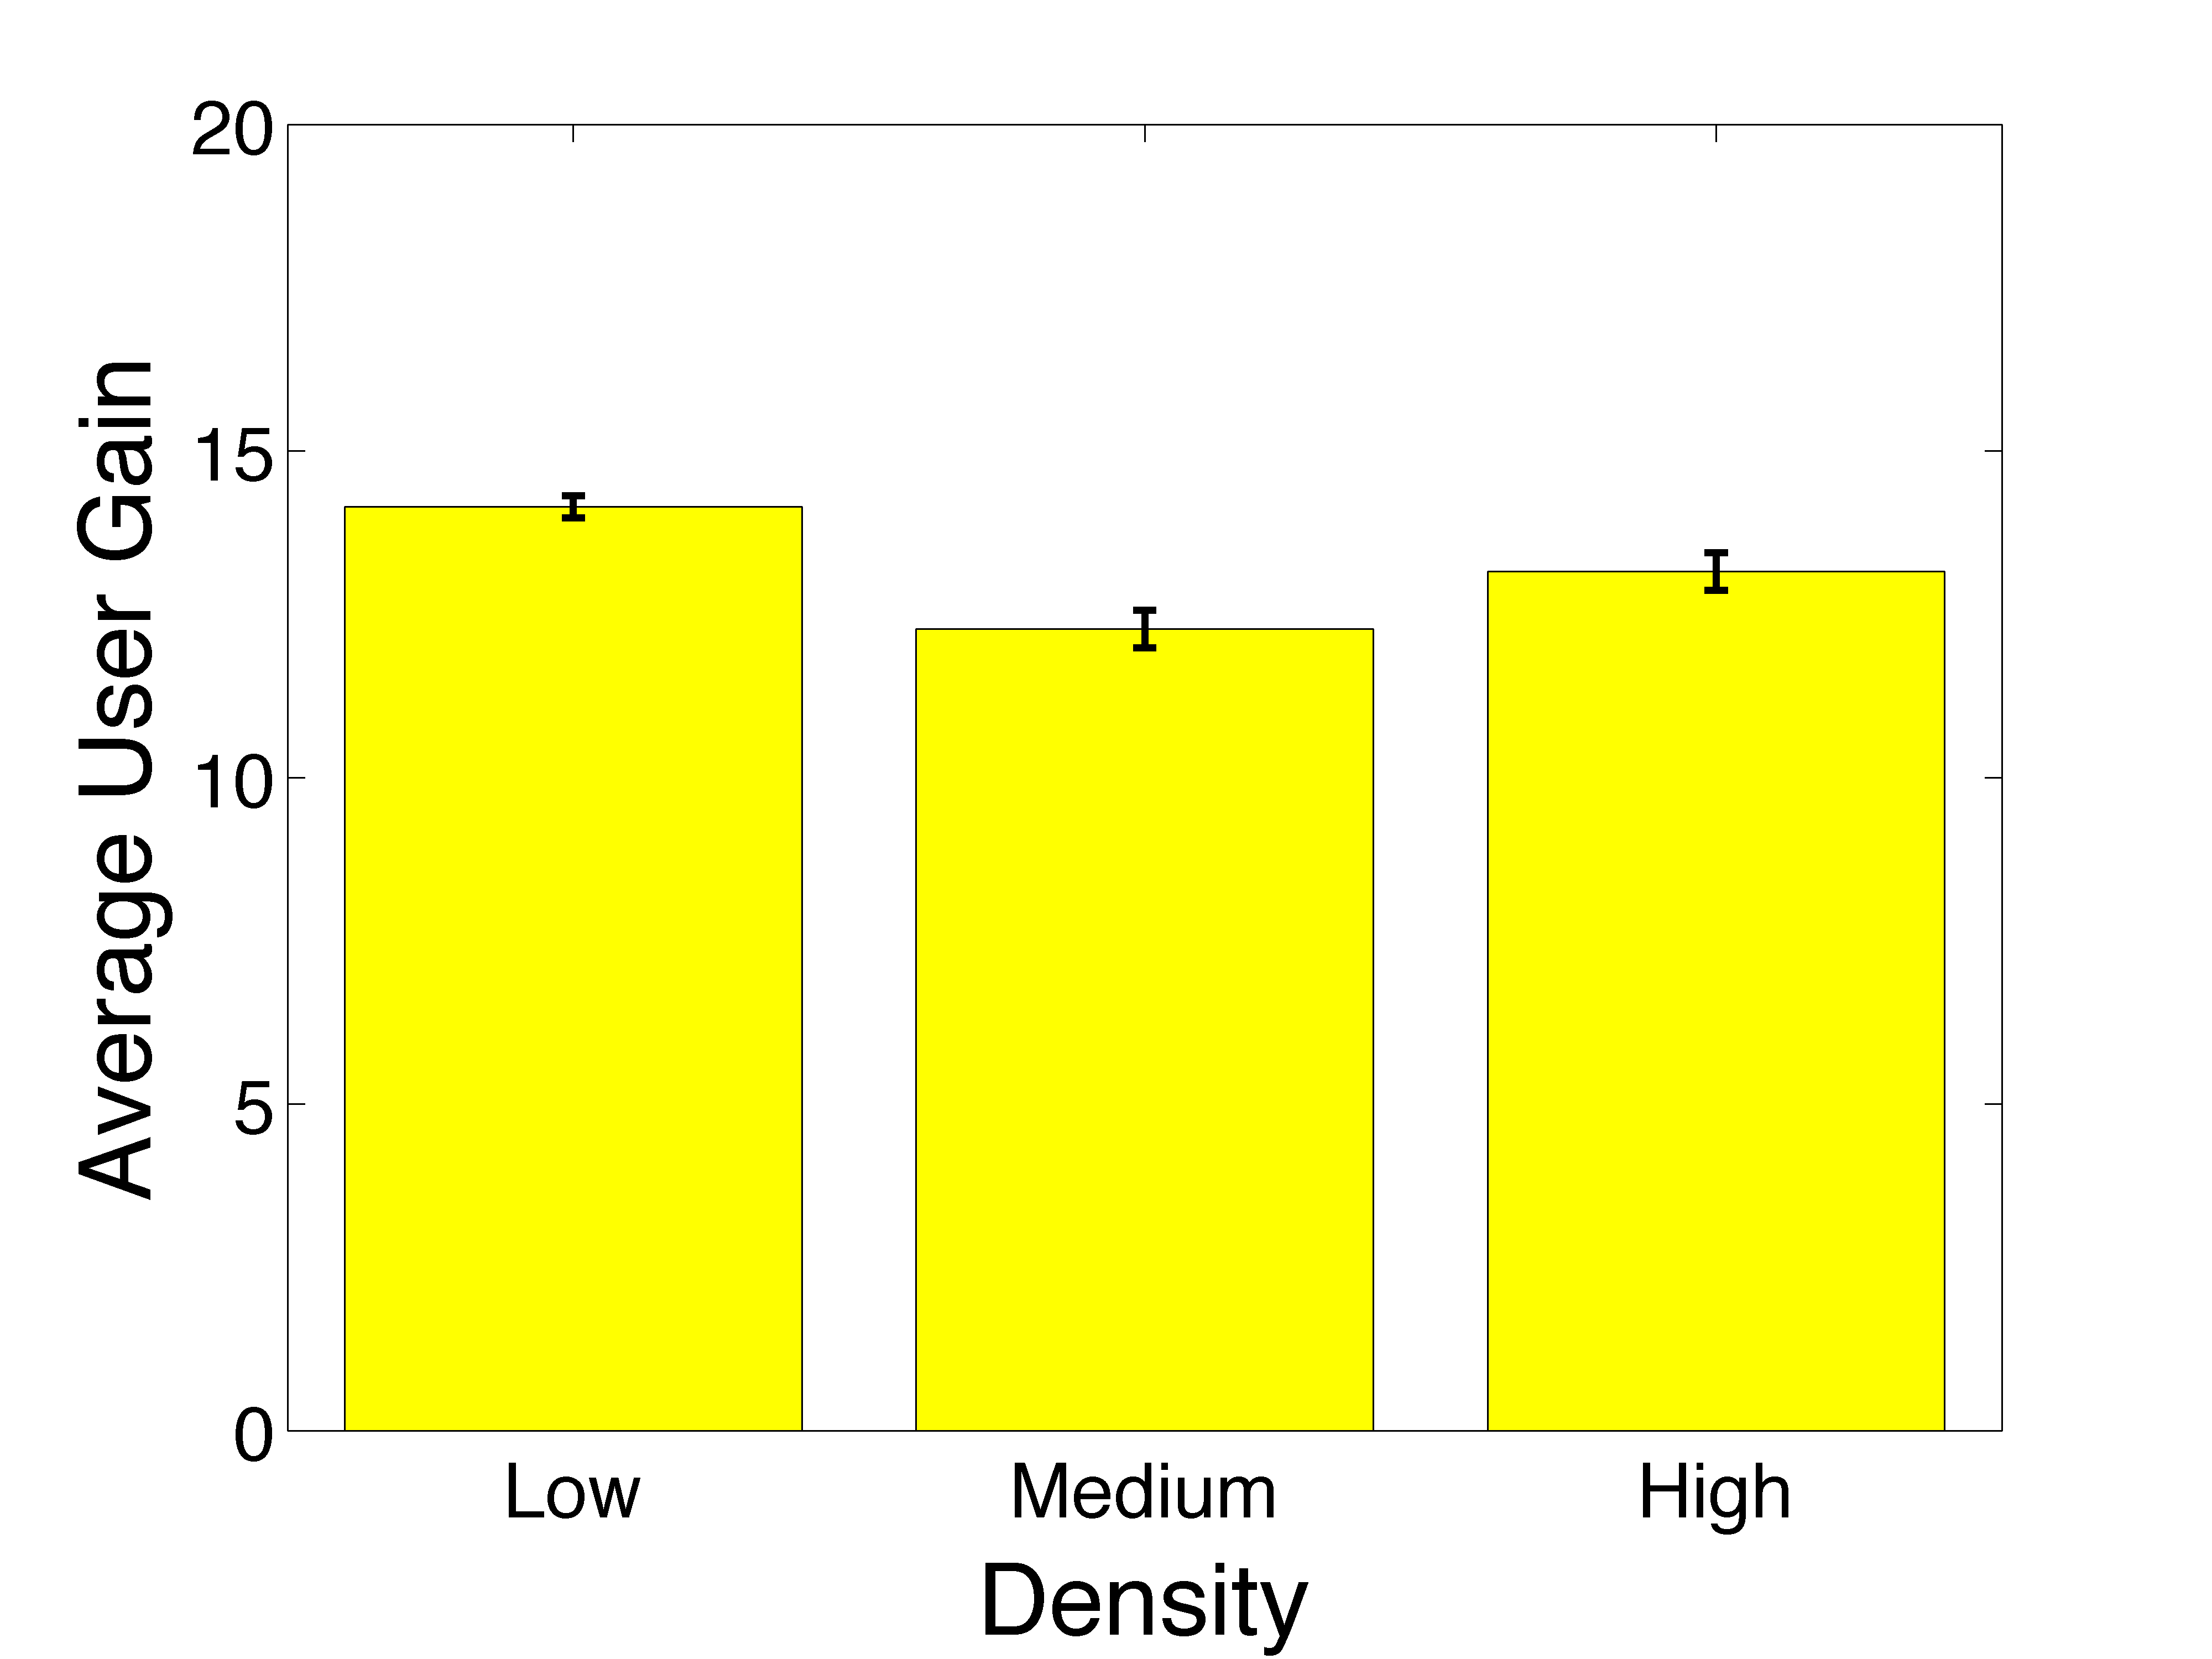
\includegraphics[width=0.33\textwidth,type=png,ext=.png,read=.png]{img/Random-1.000-AUG}
% 	}  
%   \hspace{-0.1in}\subfigure[Scale Free.]{
% 	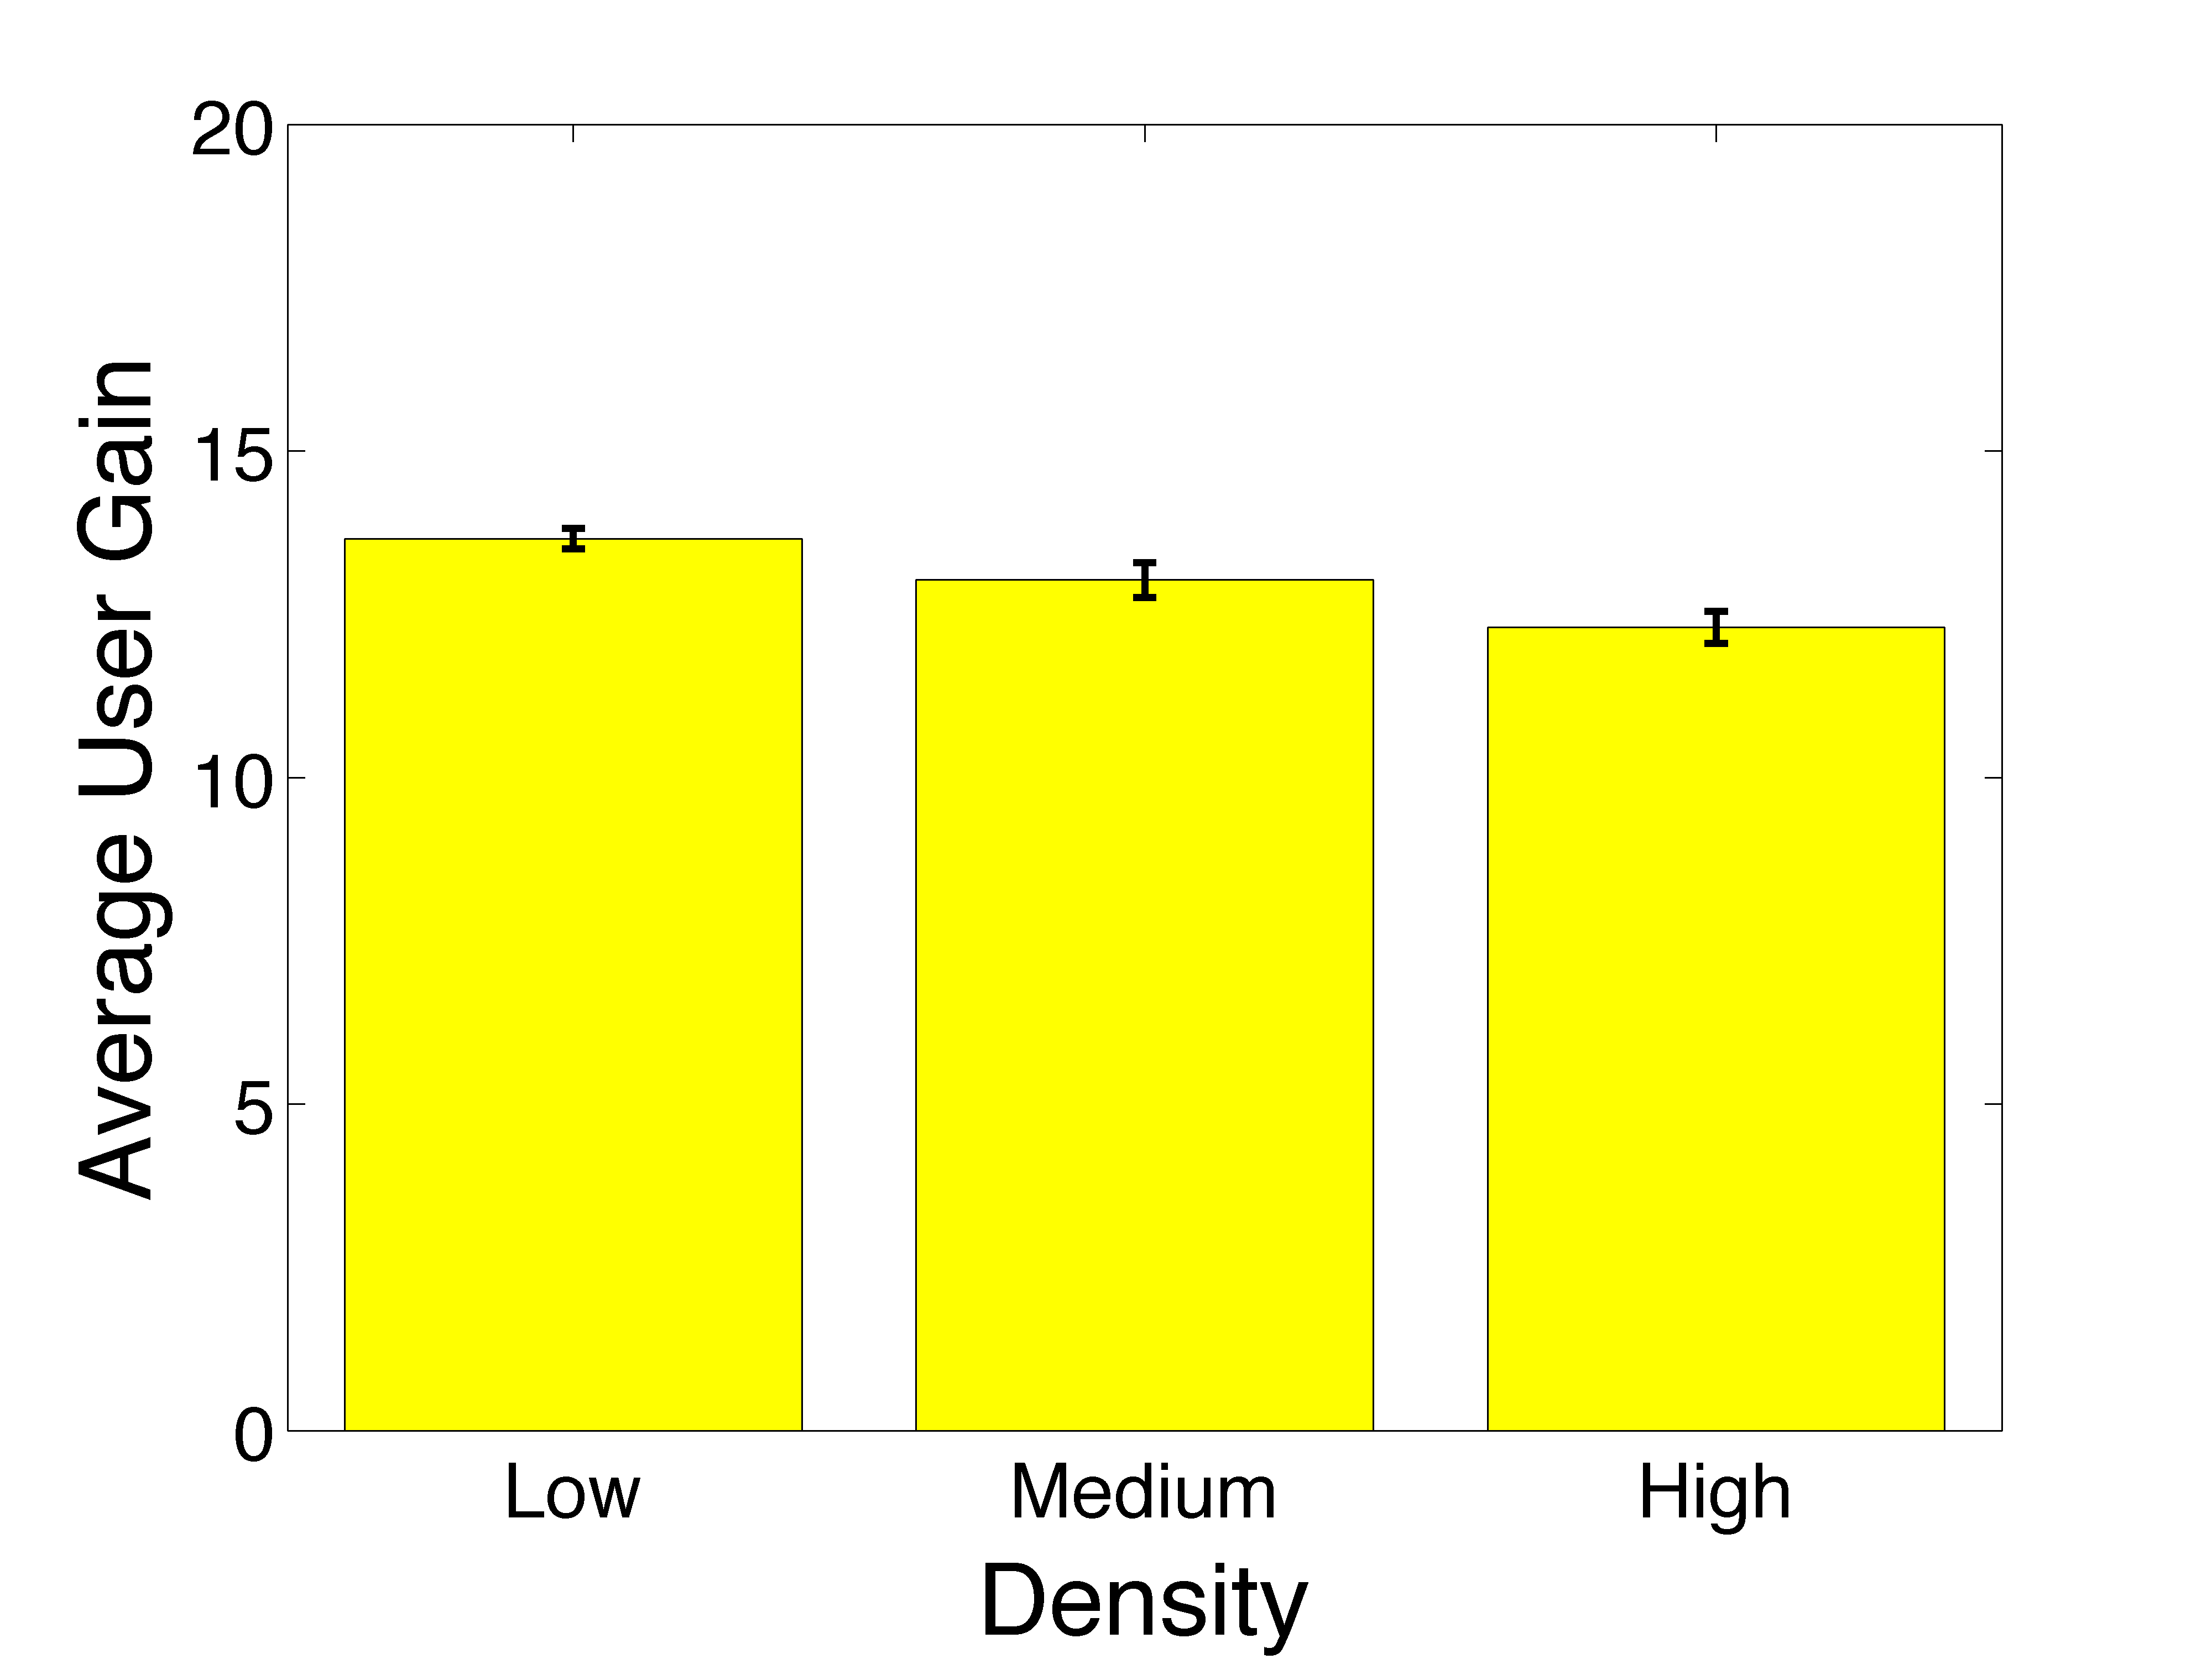
\includegraphics[width=0.33\textwidth,type=png,ext=.png,read=.png]{img/ScaleFree-1.000-AUG}
% 	}  
%   \hspace{-0.1in}\subfigure[Small World.]{
%   	%\label{fig:res_mmuca_time}
% 	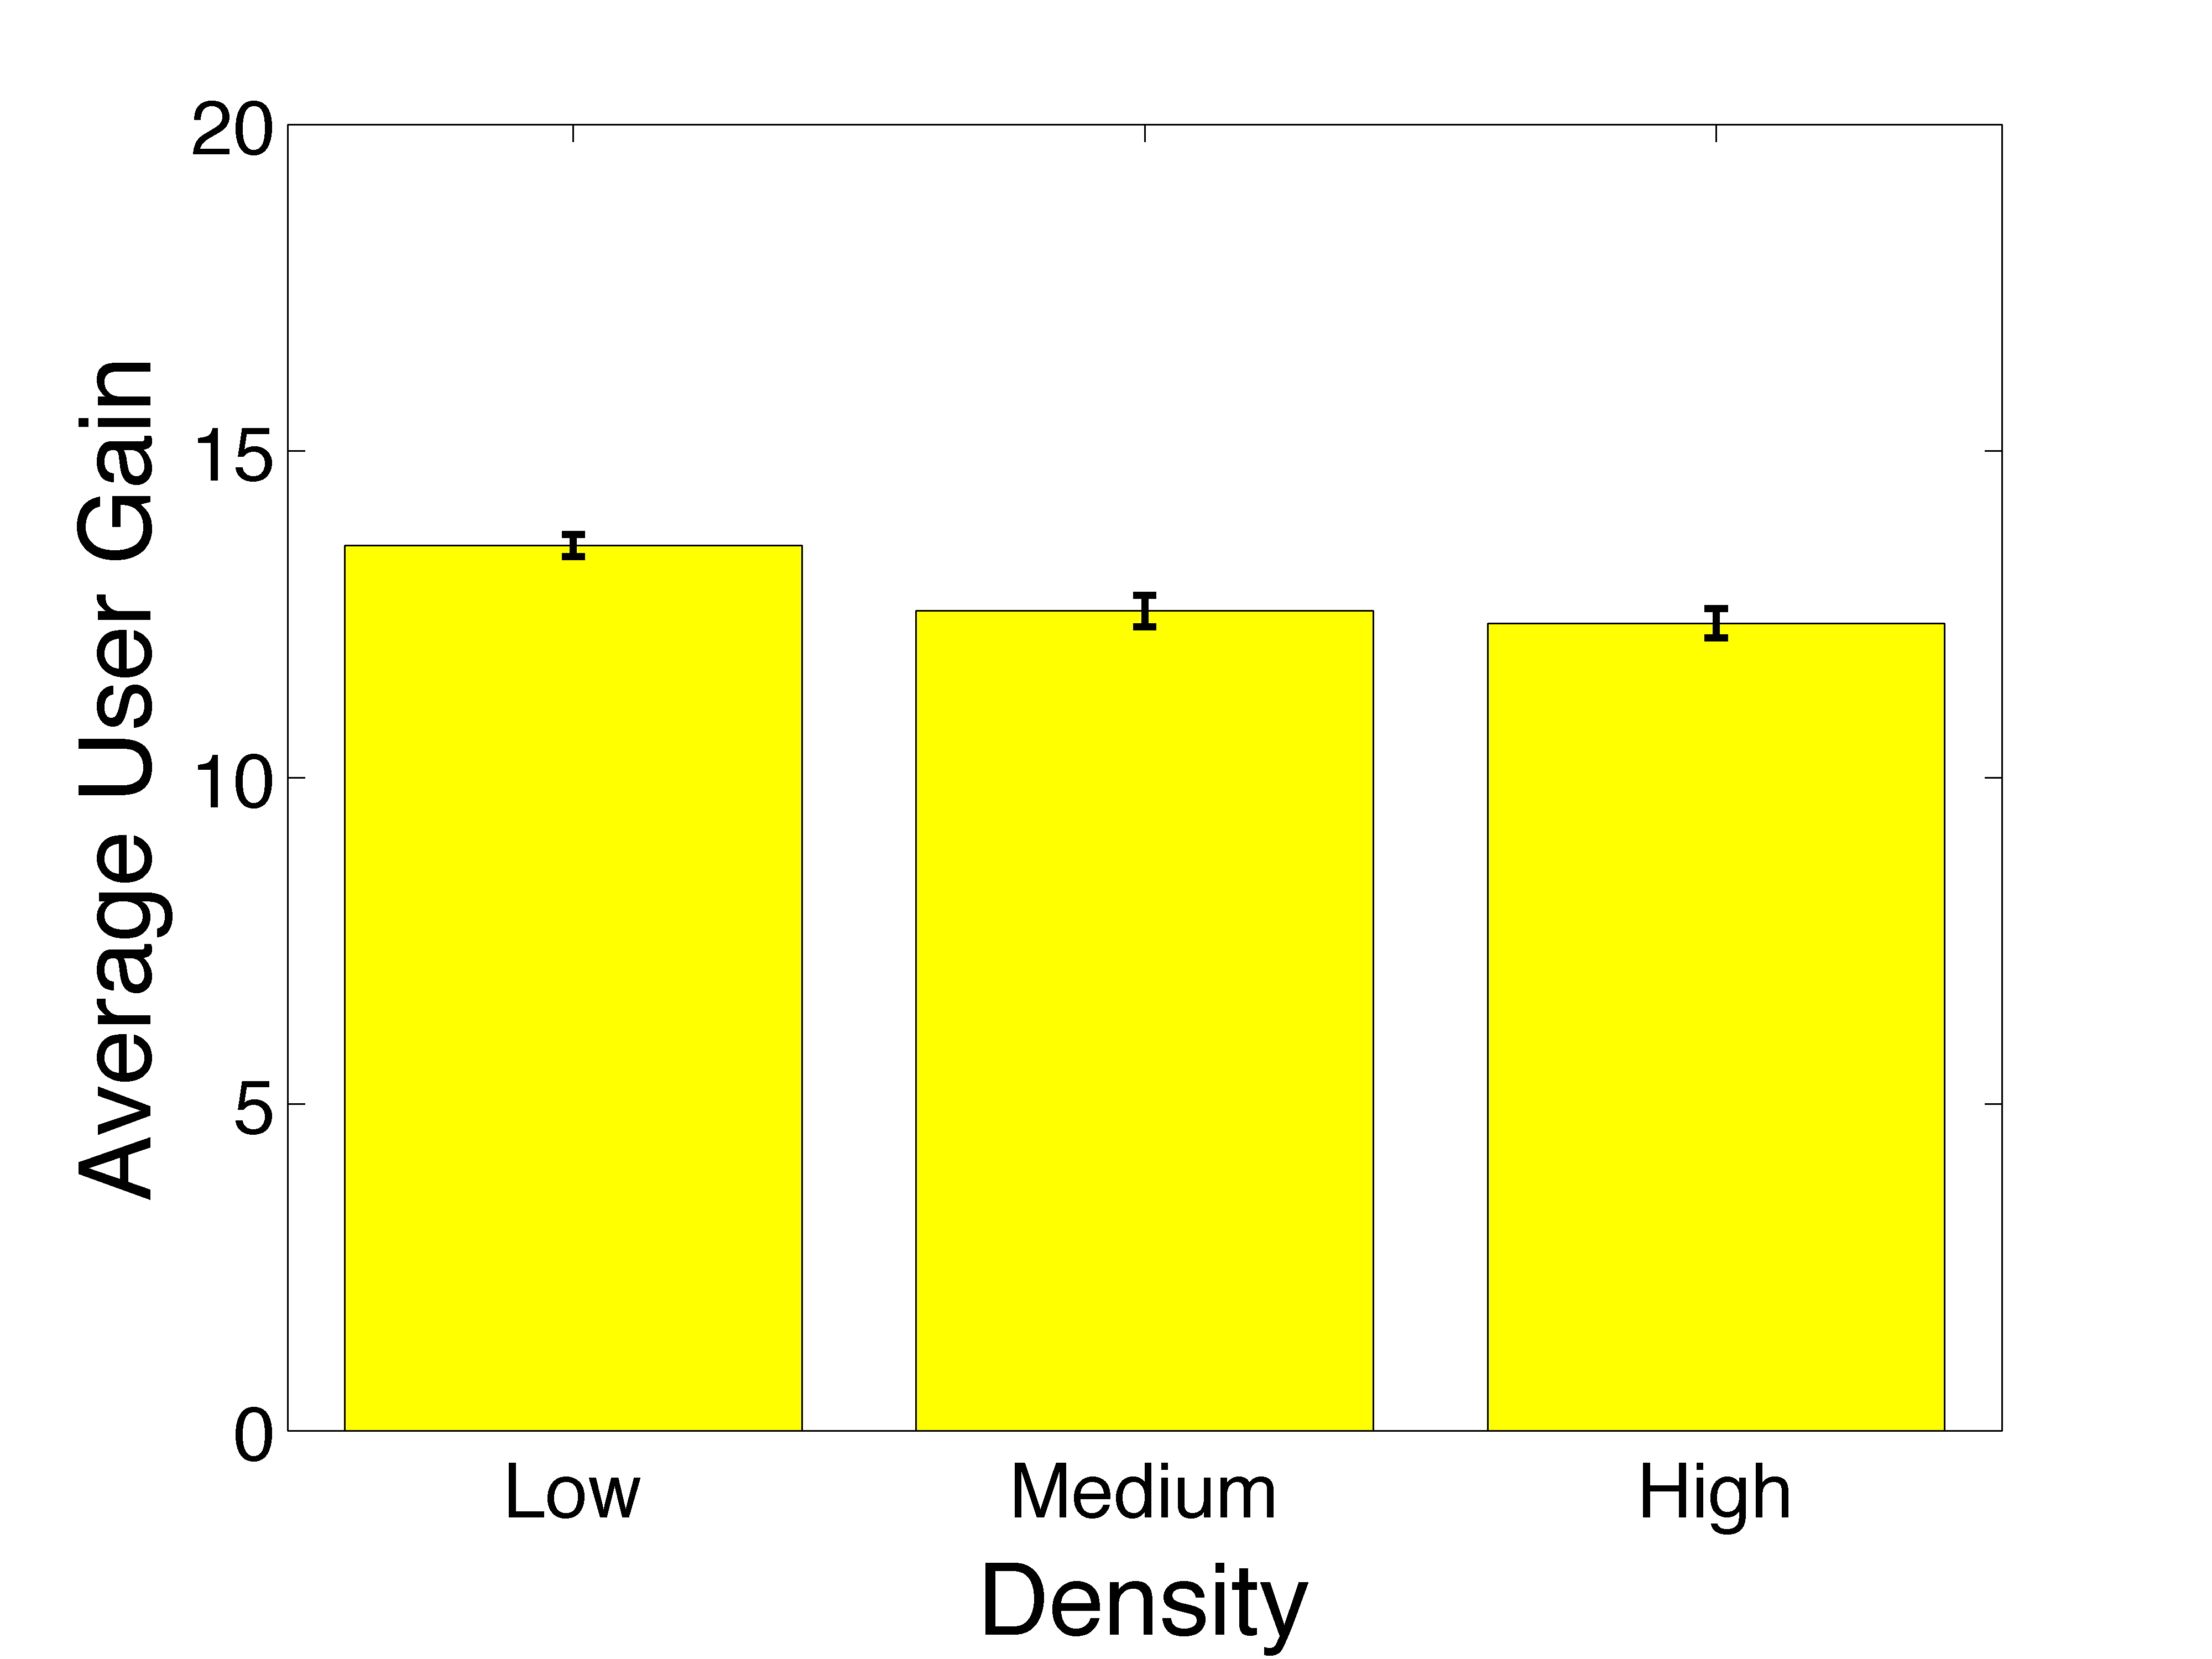
\includegraphics[width=0.33\textwidth,type=png,ext=.png,read=.png]{img/SmallWorld-1.000-AUG}
% 	}    
%   \caption{$70/80 p=1$ Graphs showing the average percent gain of consumers'
%   payoffs in the coalitions with respect to the payoff of individual coalitions on
%   different topologies and with different densities. }
%   \label{fig:graphs_gain}
% \end{figure*}
\subsubsection{Consumer's gain}

Figure \ref{fig:graphs_gain} show the results
for 12 agents on a random, scale-free and small-world networks in the three
different market scenarios respectively.
We also plotted the standard error of the mean as a measure of the
variance in each graph. Only data regarding instances with non-empty core are
plotted. Observe that in all configurations, although the average percent user
gain is increased with density, this increment is not significant. Moreover, the
average percent user gain is much higher (around $10\%$) in $M_3$ market than not
in $M_1$ and $M_2$ (around $1\%$).

% Each graph shows the
% mean
%among the from 50 problem instances that resulted in non-empty core of the user
%percent gain of consumers in coalitions with respect to their individual
%coalitions when varying the density of the agent's social network.

%As expected graphs show that increasing the network social density increases
% the percent user gain in all scenarios because each new link allows the formation of
%a set of new energy coalitions that were forbidden before. However this
%increment of gain is more significant on random graphs and small world networks
%where the degree of nodes is more uniform than not in scale free due to the
%presence of hubs.

\subsubsection{Core emptiness}
Table \ref{tab:percentage_core_emptiness} shows the percentage of
instances under each configuration for which the core was detected as empty.
Notice that in all network topologies, the number of instances for which the core is empty
increases with the density of the network. These results are coherent with the
well-known results that any acyclic network (which has by definition the
lowest density) is guarantee to have a non-empty core \cite{RePEc:ucp:jpolec:v:112:y:2004:i:4:p:754-778}. As we
increase the density the number of cycles also increase and results show that the probability
of core emptiness is higher.
Regarding different network topologies, we observe that the number of instances
with core emptiness is higher in scale free networks, where the links are
concentrated on hubs, than not on random and small-world networks, where each
node in average have the same degree.
Finally, we also observe that the number of instances with core empty is much
higher on $M_1$ and $M_2$ than not in $M_3$. Although we need to perform a deeper
analysis on these results, they lead to the hypothesis that the more the
distance of prices in the market the less the probability of having an empty
core in the coalitional game.

\begin{table}[!ht]
\centering
\begin{tabular}{ | c | c | c |  c | c |}
\hline
\multirow{2}{*}{\textbf{Topology}} & \multirow{2}{*}{\textbf{Density}}&\multicolumn{3}{c|}{ \textbf{$\%$   Empty Core}}\\
\cline{3-5}
& & $M_1$ & $M_2$ & $M_3$ \\
\hline
\multirow{3}{*}{Random} & Low &  $  8\%$ & $ 0\% $ & $ 0\% $ \\
 & Medium &  $  50\%$ & $ 26\% $ & $ 6\% $ \\
 & High &  $  56\%$ & $ 44\% $ & $ 10\% $ \\
\hline
\multirow{3}{*}{Scale-Free} & Low &  $  0\%$ & $ 0\% $ & $ 0\% $ \\
 & Medium &  $  52\%$ & $ 22\% $ & $ 2\% $ \\
 & High &  $  46\%$ & $ 38\% $ & $ 12\% $ \\
\hline
\multirow{3}{*}{Small-World} & Low &  $  8\%$ & $ 6\% $ & $ 2\% $ \\
 & Medium &  $  46\%$ & $ 18\% $ & $ 8\% $ \\
 & High &  $  46\%$ & $ 48\% $ & $ 6\% $ \\
\hline
\end{tabular}
\caption{\label{tab:percentage_core_emptiness} Percentage of instances with empty core under different configurations.}
\end{table}

\subsubsection{Structure of energy coalitions}
In this section we analyze the structure of the energy coalitions obtained in
the experiments. For each configuration, we plot the mean of the minimum,
average and maximum size of coalitions formed. Figure \ref{fig:graphs_size}
plots the results for networks of 12 agents on a random, scale free and
small-world networks in two different market scenarios. We also plotted
the standard error of the mean as a measure of the variance in each graph.
Market scenario $M_3$ is omitted because in this case we detected that the gran coalition was always formed in all tested instances.

\noindent Since the difference between $p_{DA}$ and $p_{F}$ in $M_3$ is relatively high, buying more energy in the forward market is very profitable, leading to the formation of bigger coalitions. In contrast we observe that for markets $M_1$ and $M_2$, the market conditions lead to
coalitions of middle size in all network structures. We also observe that as we
increase the density of the network, more coalitions of middle size are composed
whereas in low densities agents tend to compose larger coalitions.

\section{Plots}

\begin{figure*} [!h] 
  \centering
  \vspace{-0.1in}
  \hspace{-0.1in}\subfigure[Random Graphs $M_1$]{
	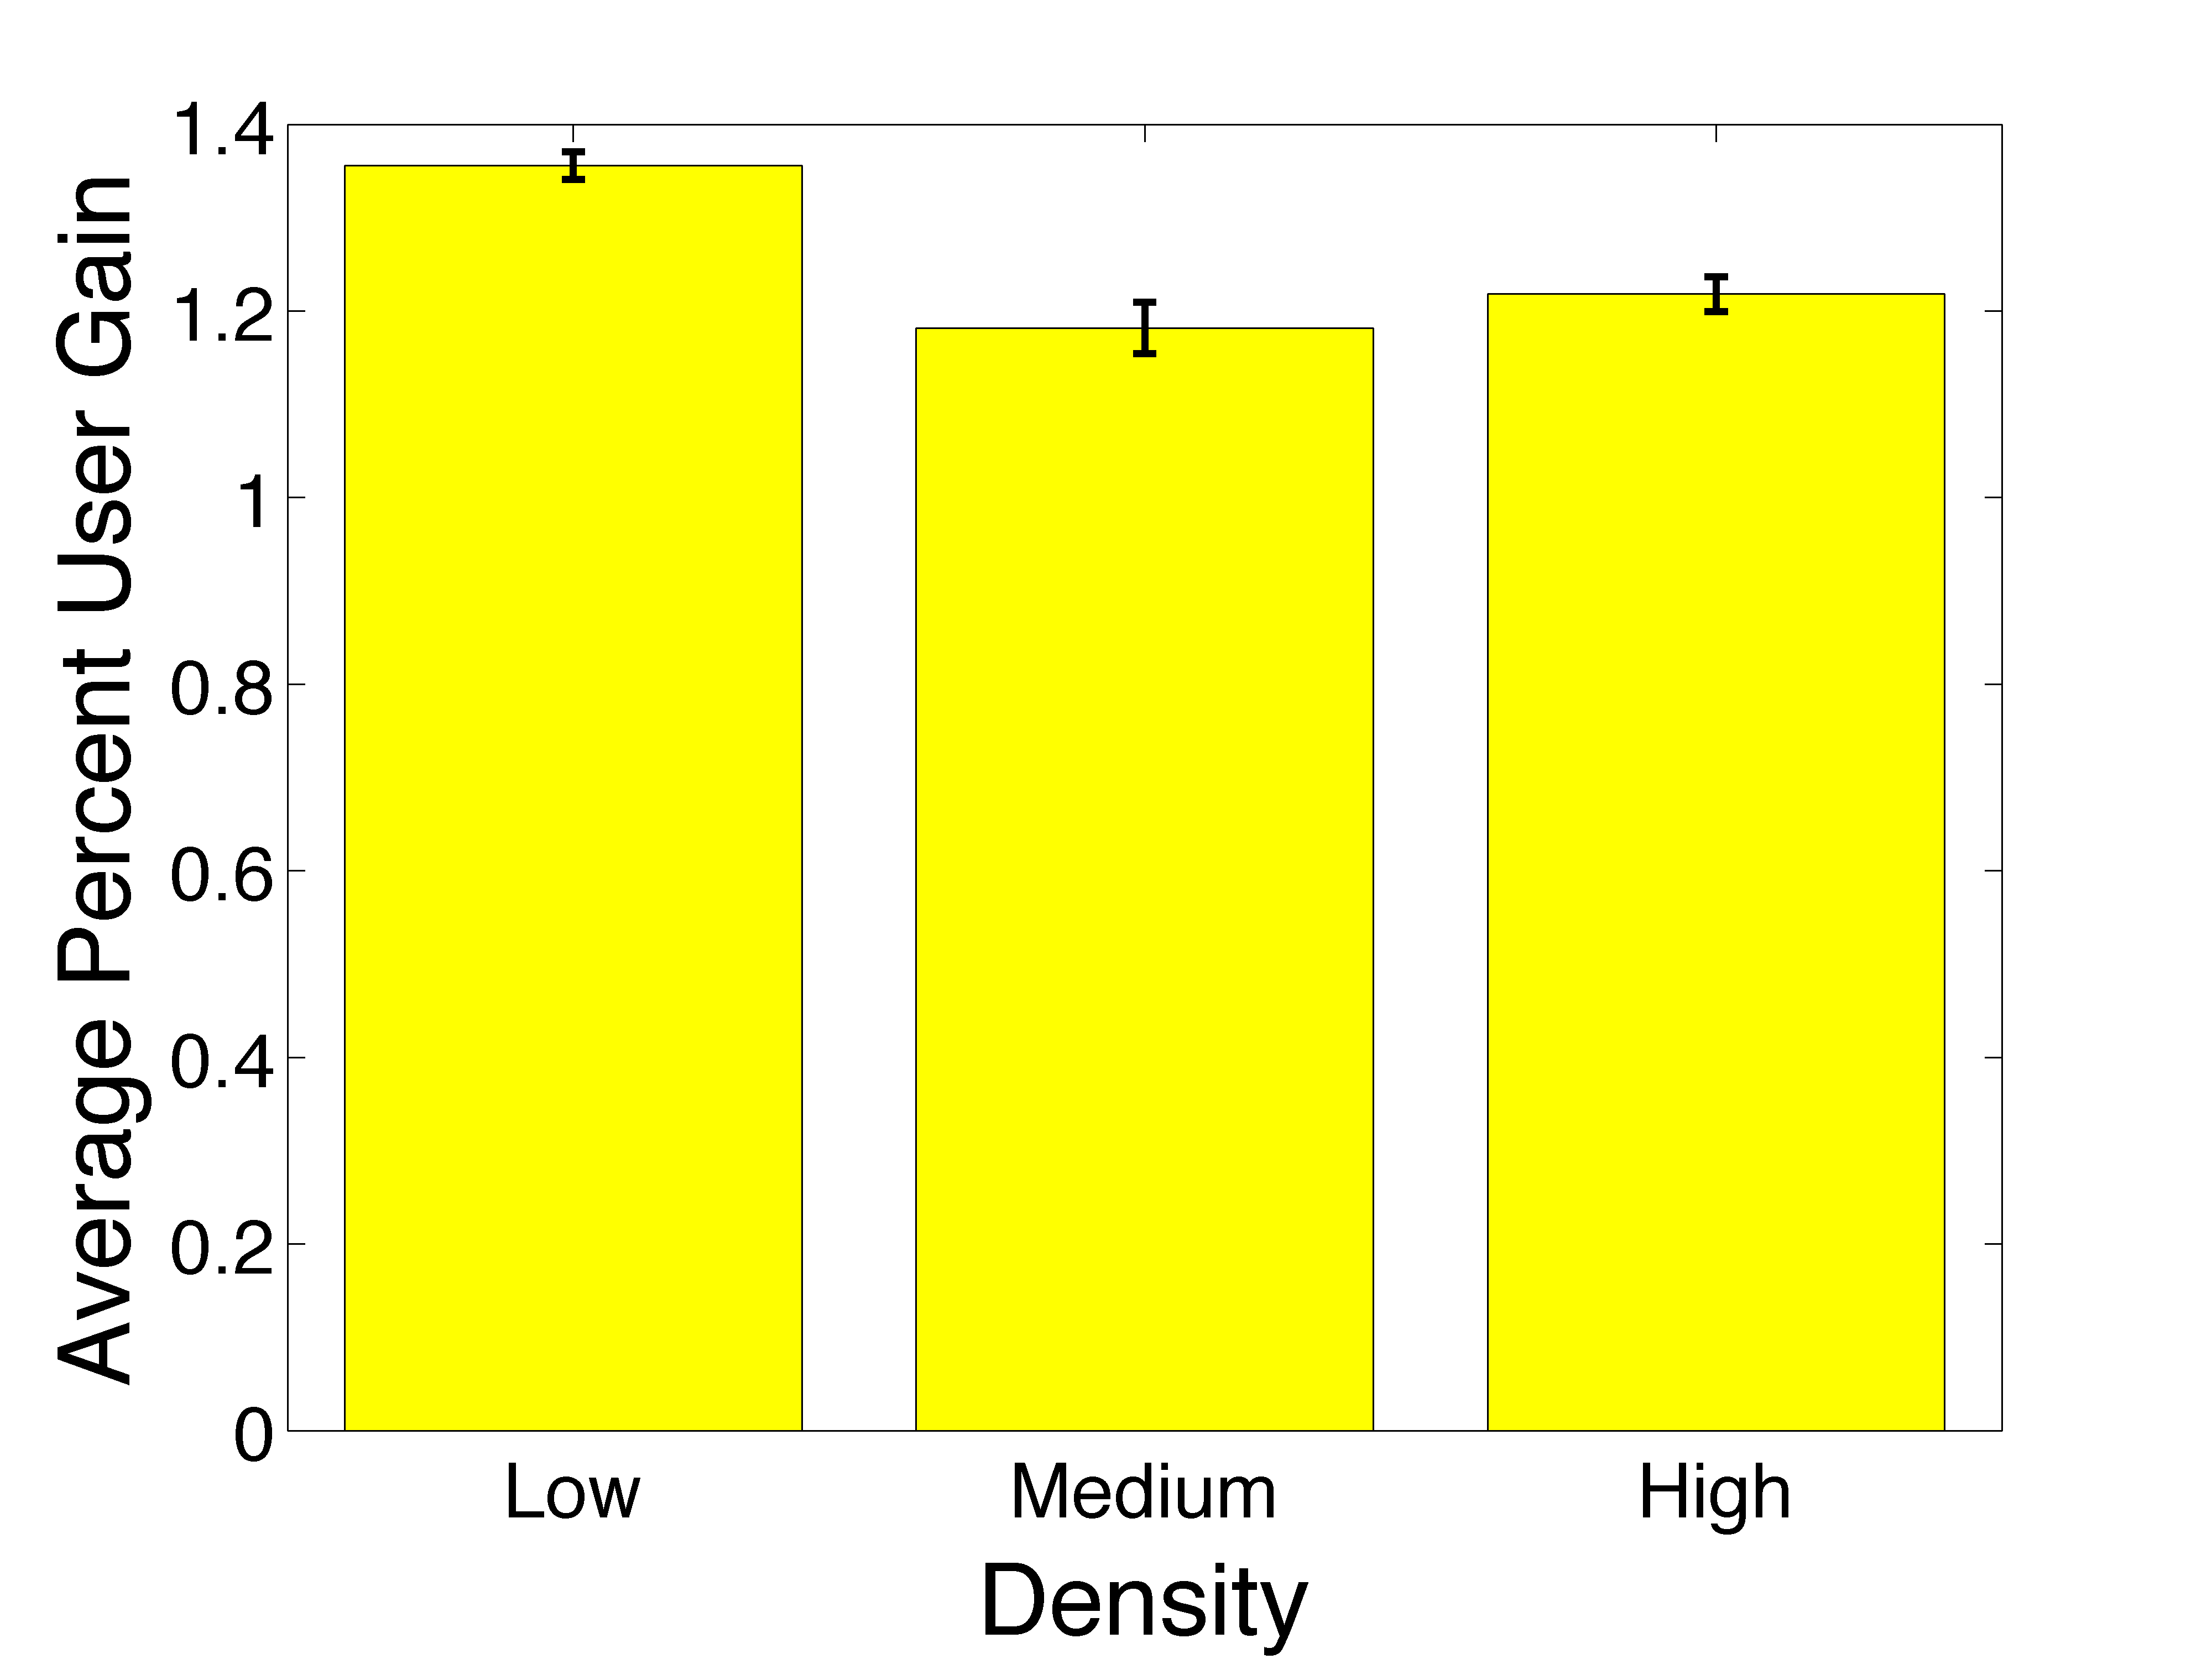
\includegraphics[width=0.32\textwidth,type=png,ext=.png,read=.png]{graphs/Random-1.000-AUG-PER}
	}  
  \hspace{-0.1in}\subfigure[Scale Free $M_1$]{
	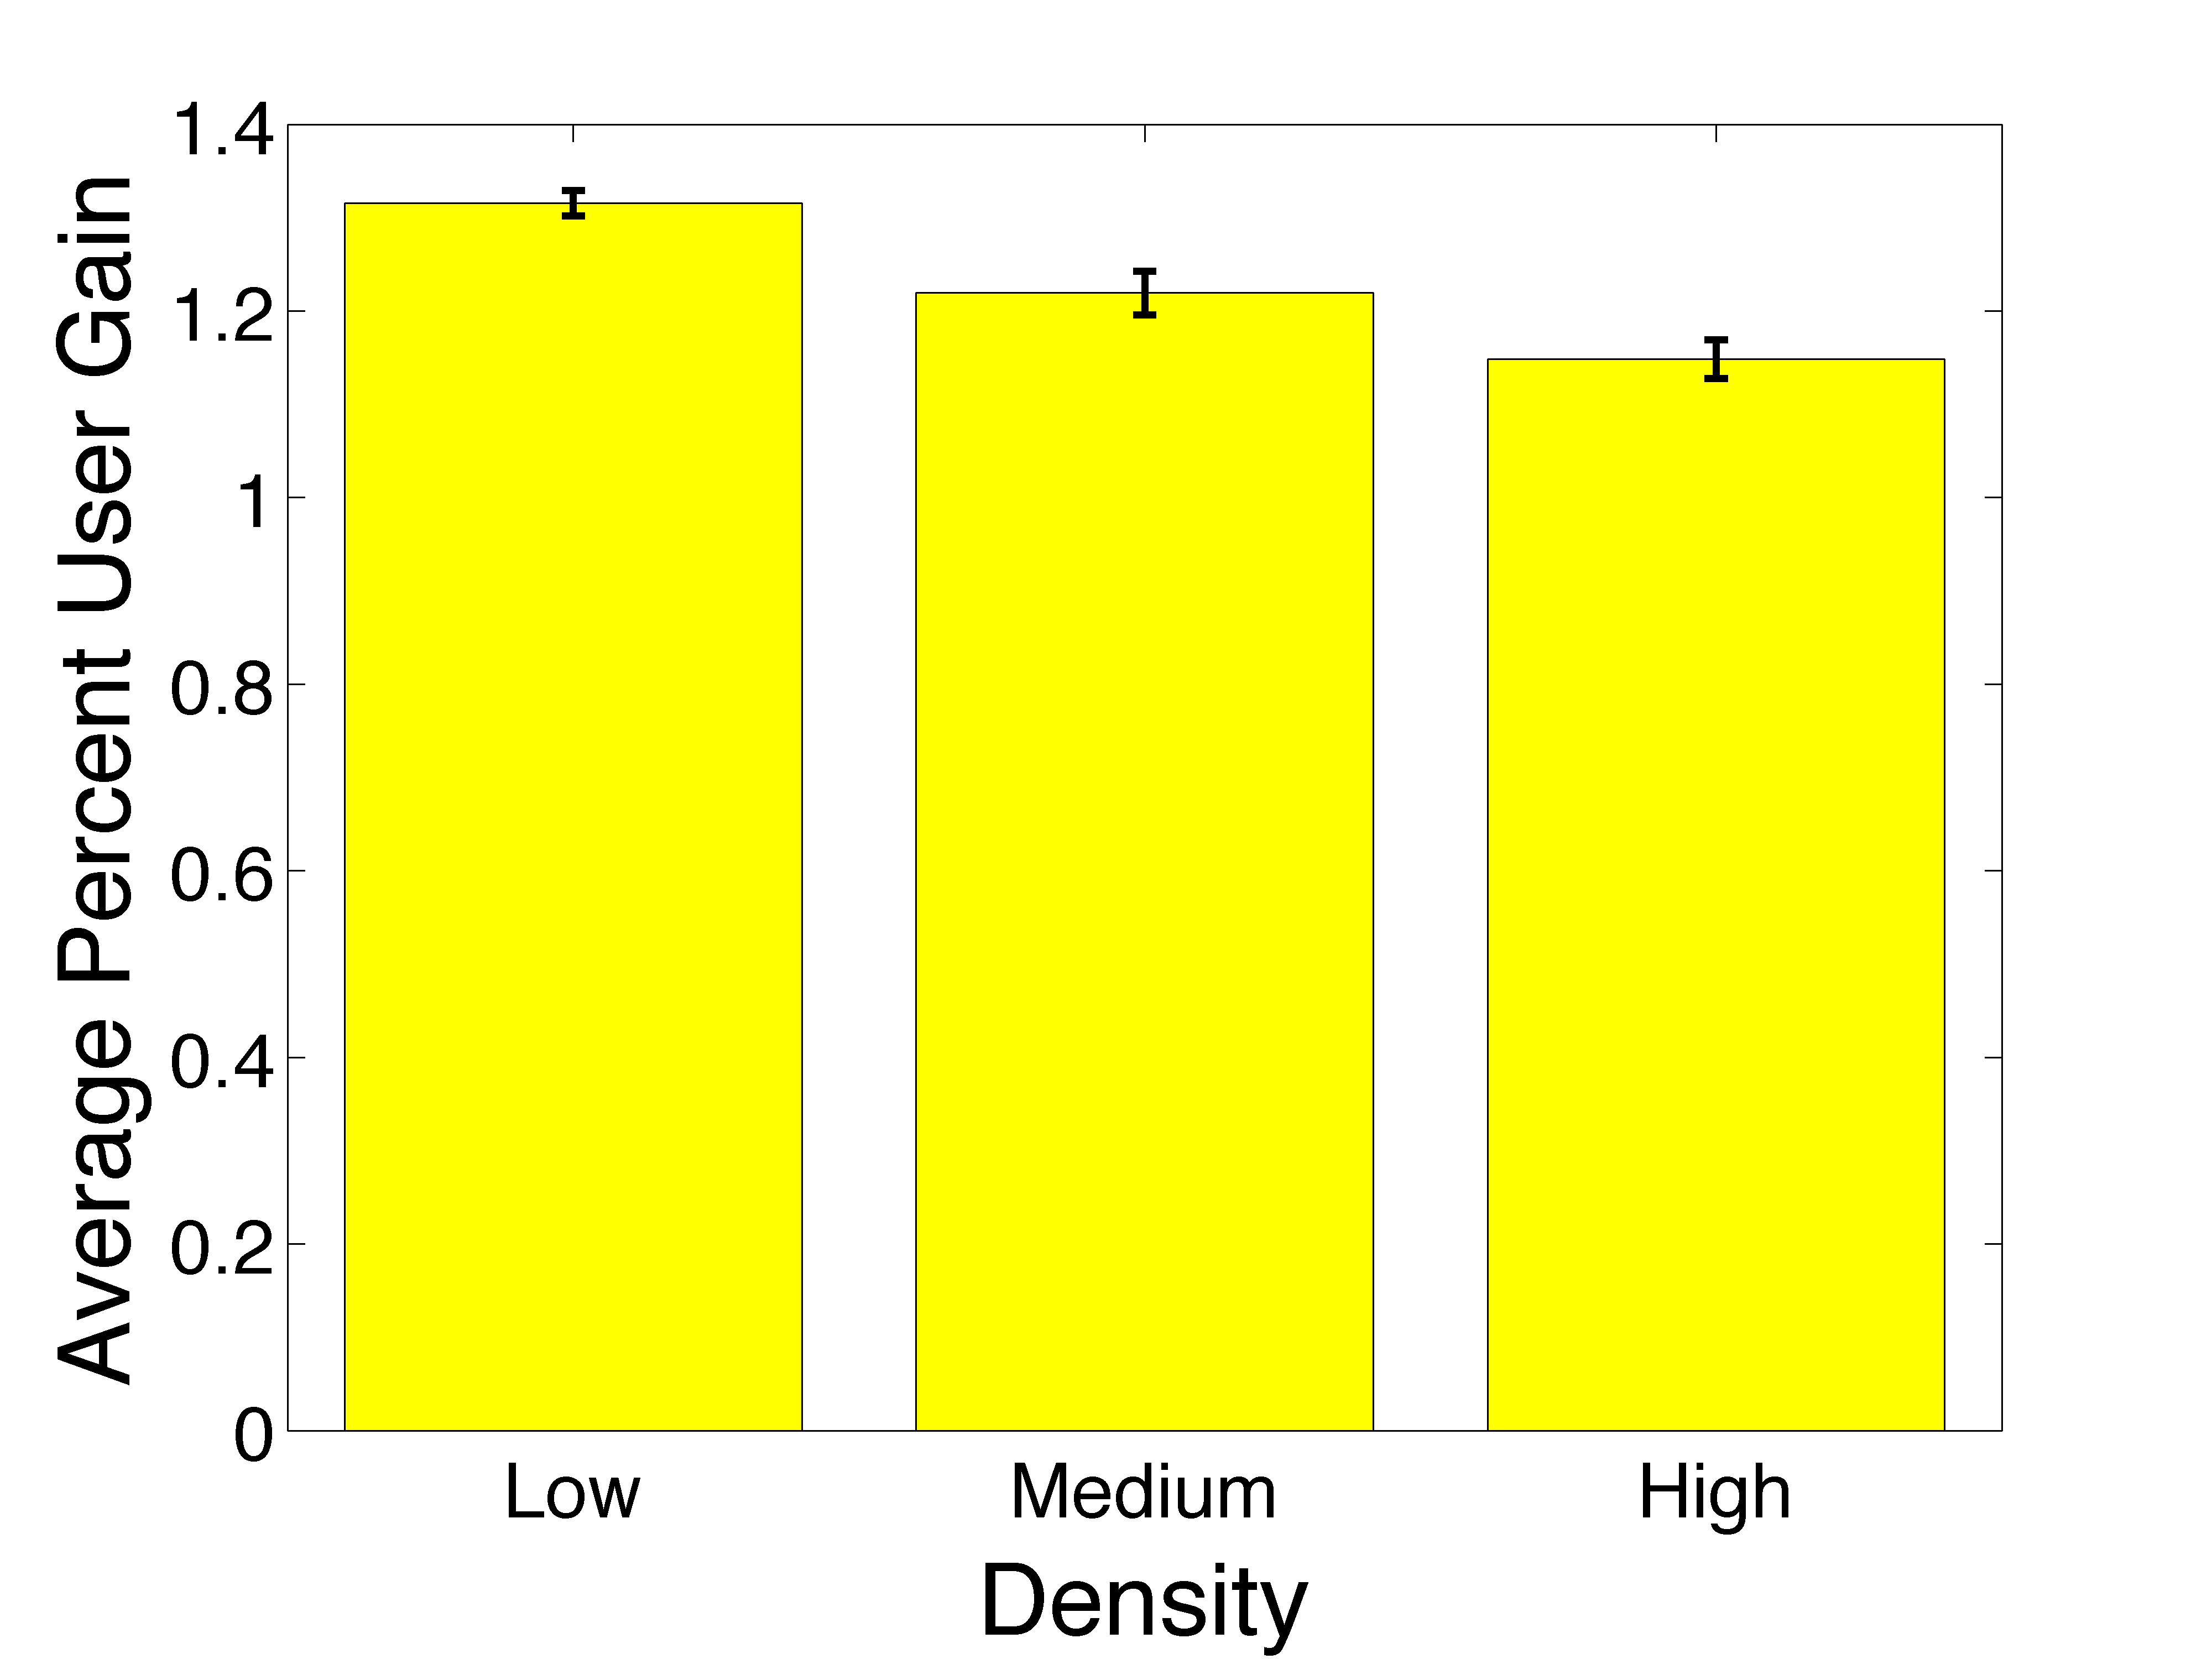
\includegraphics[width=0.32\textwidth,type=png,ext=.png,read=.png]{graphs/ScaleFree-1.000-AUG-PER}
	}  
  \hspace{-0.1in}\subfigure[Small World $M_1$]{
	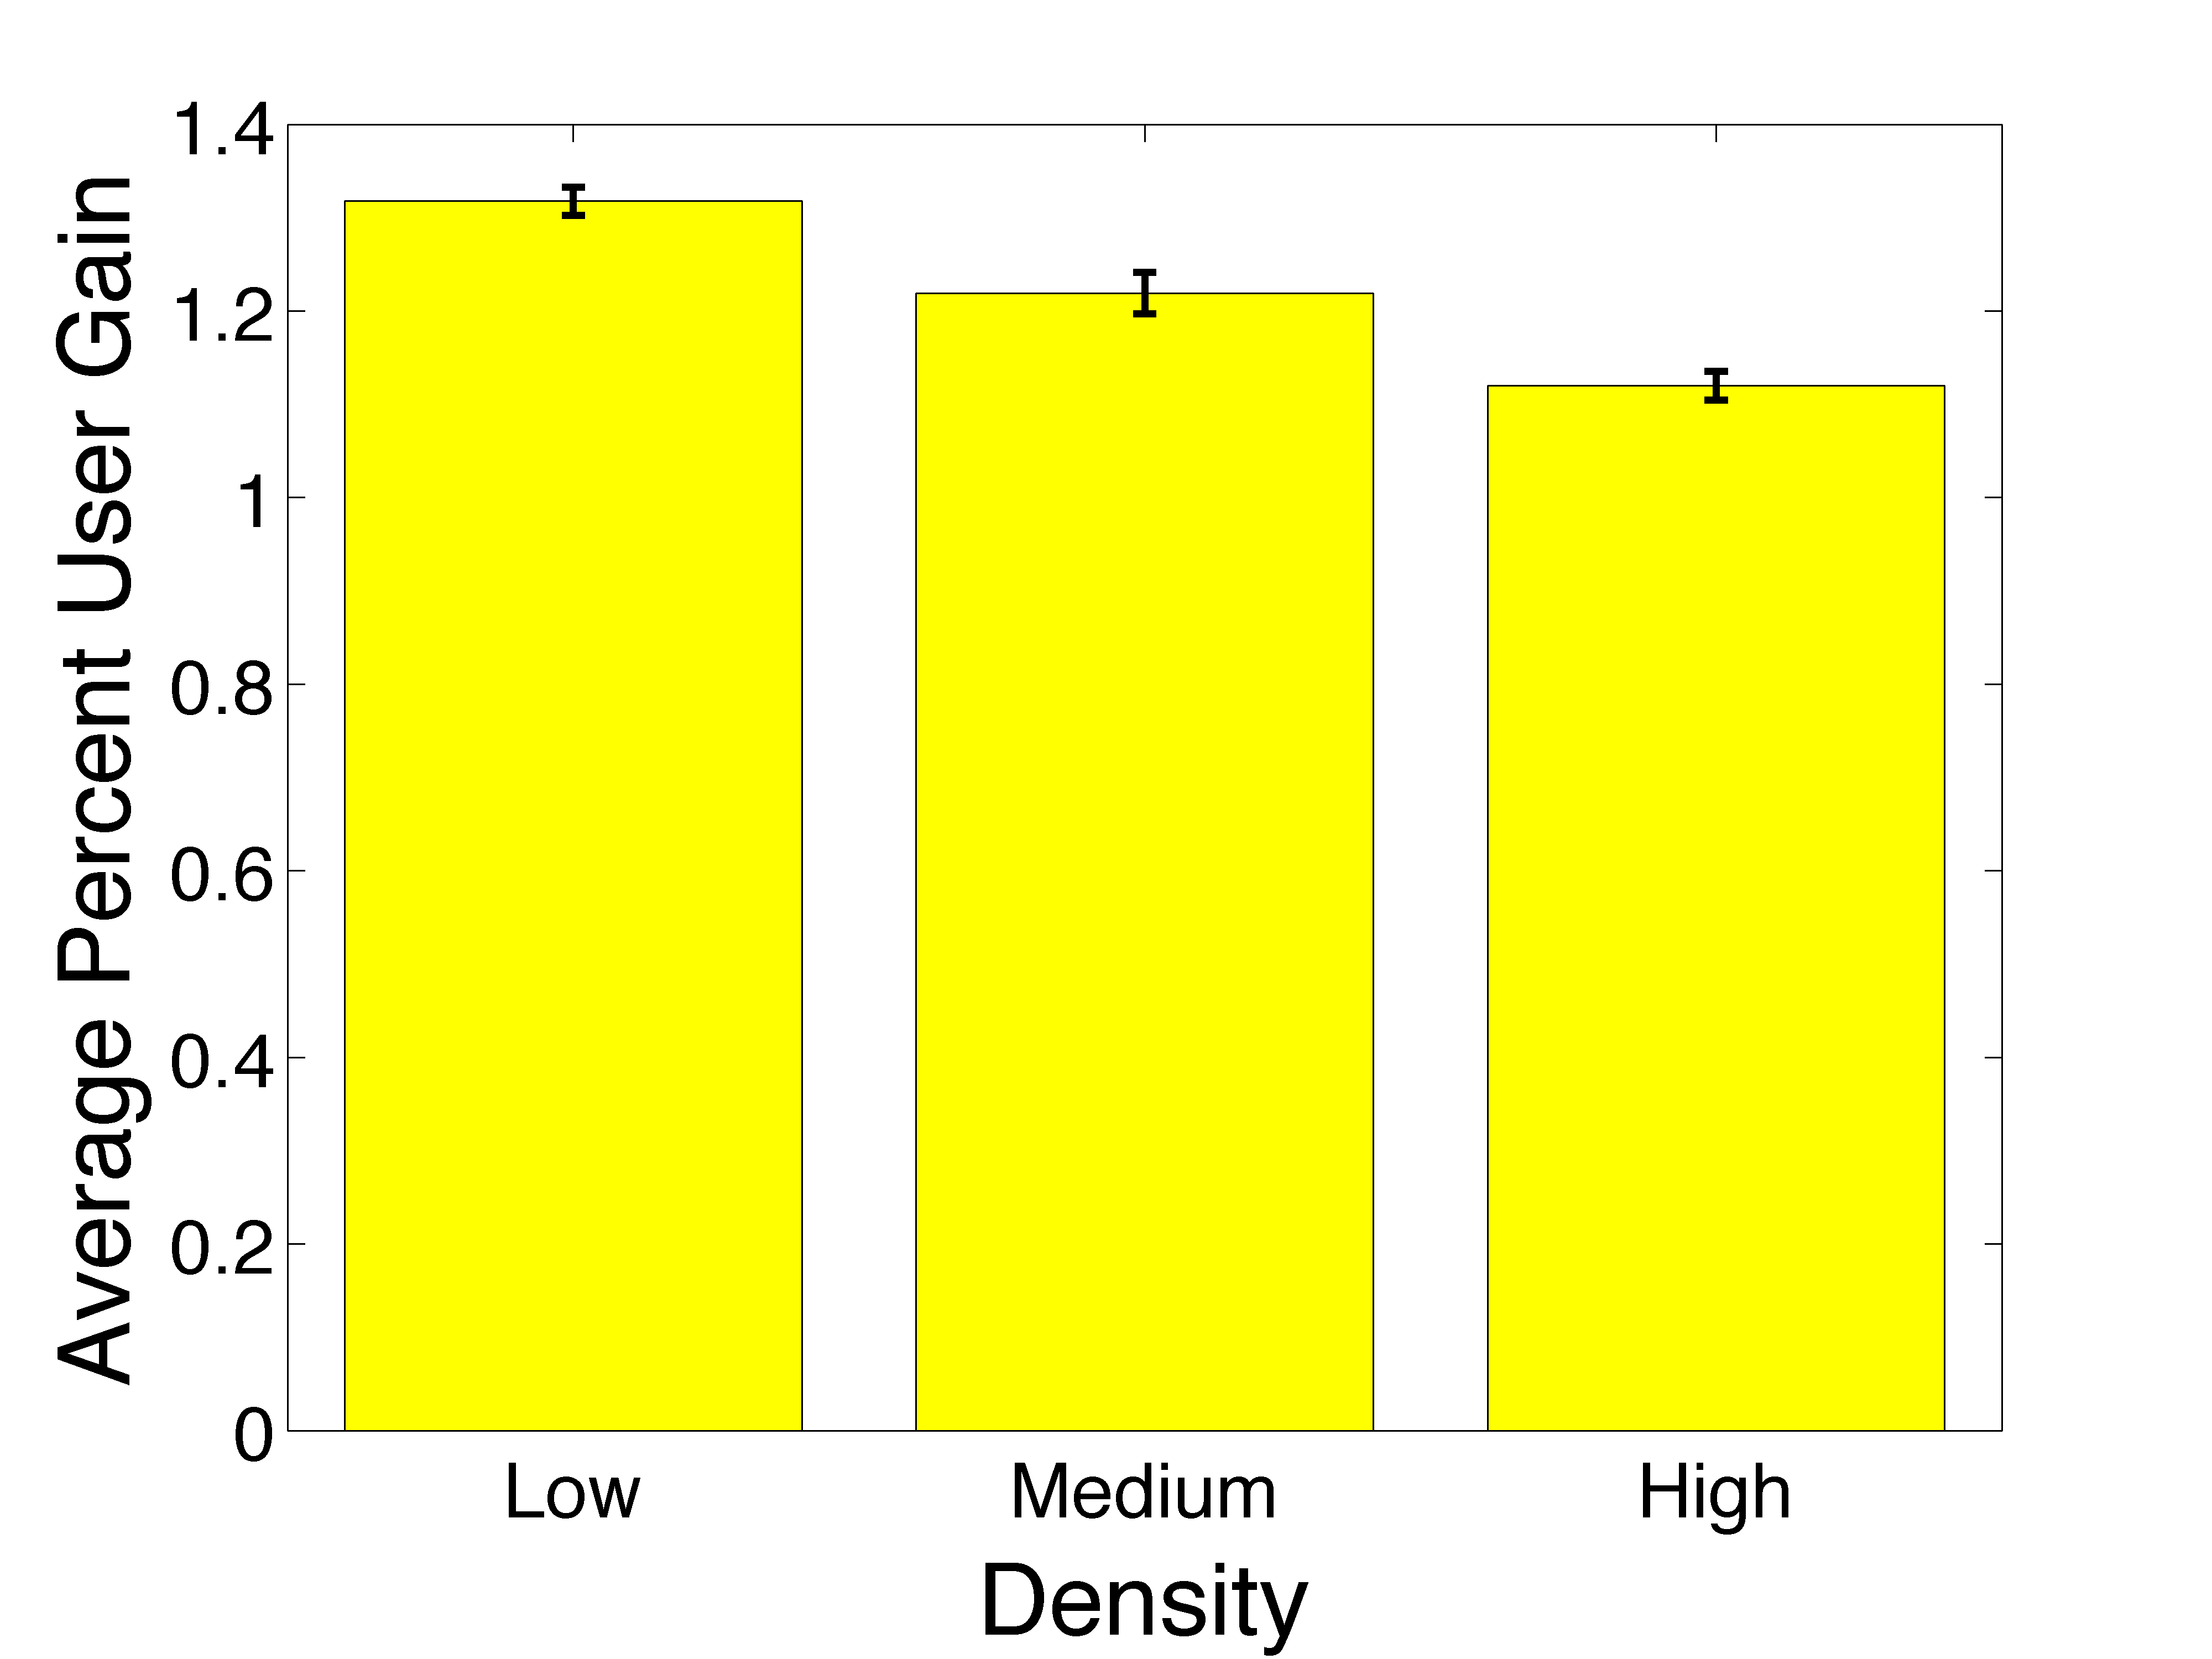
\includegraphics[width=0.32\textwidth,type=png,ext=.png,read=.png]{graphs/SmallWorld-1.000-AUG-PER}
	}
	
  \hspace{-0.1in}\subfigure[Random Graphs $M_2$]{
	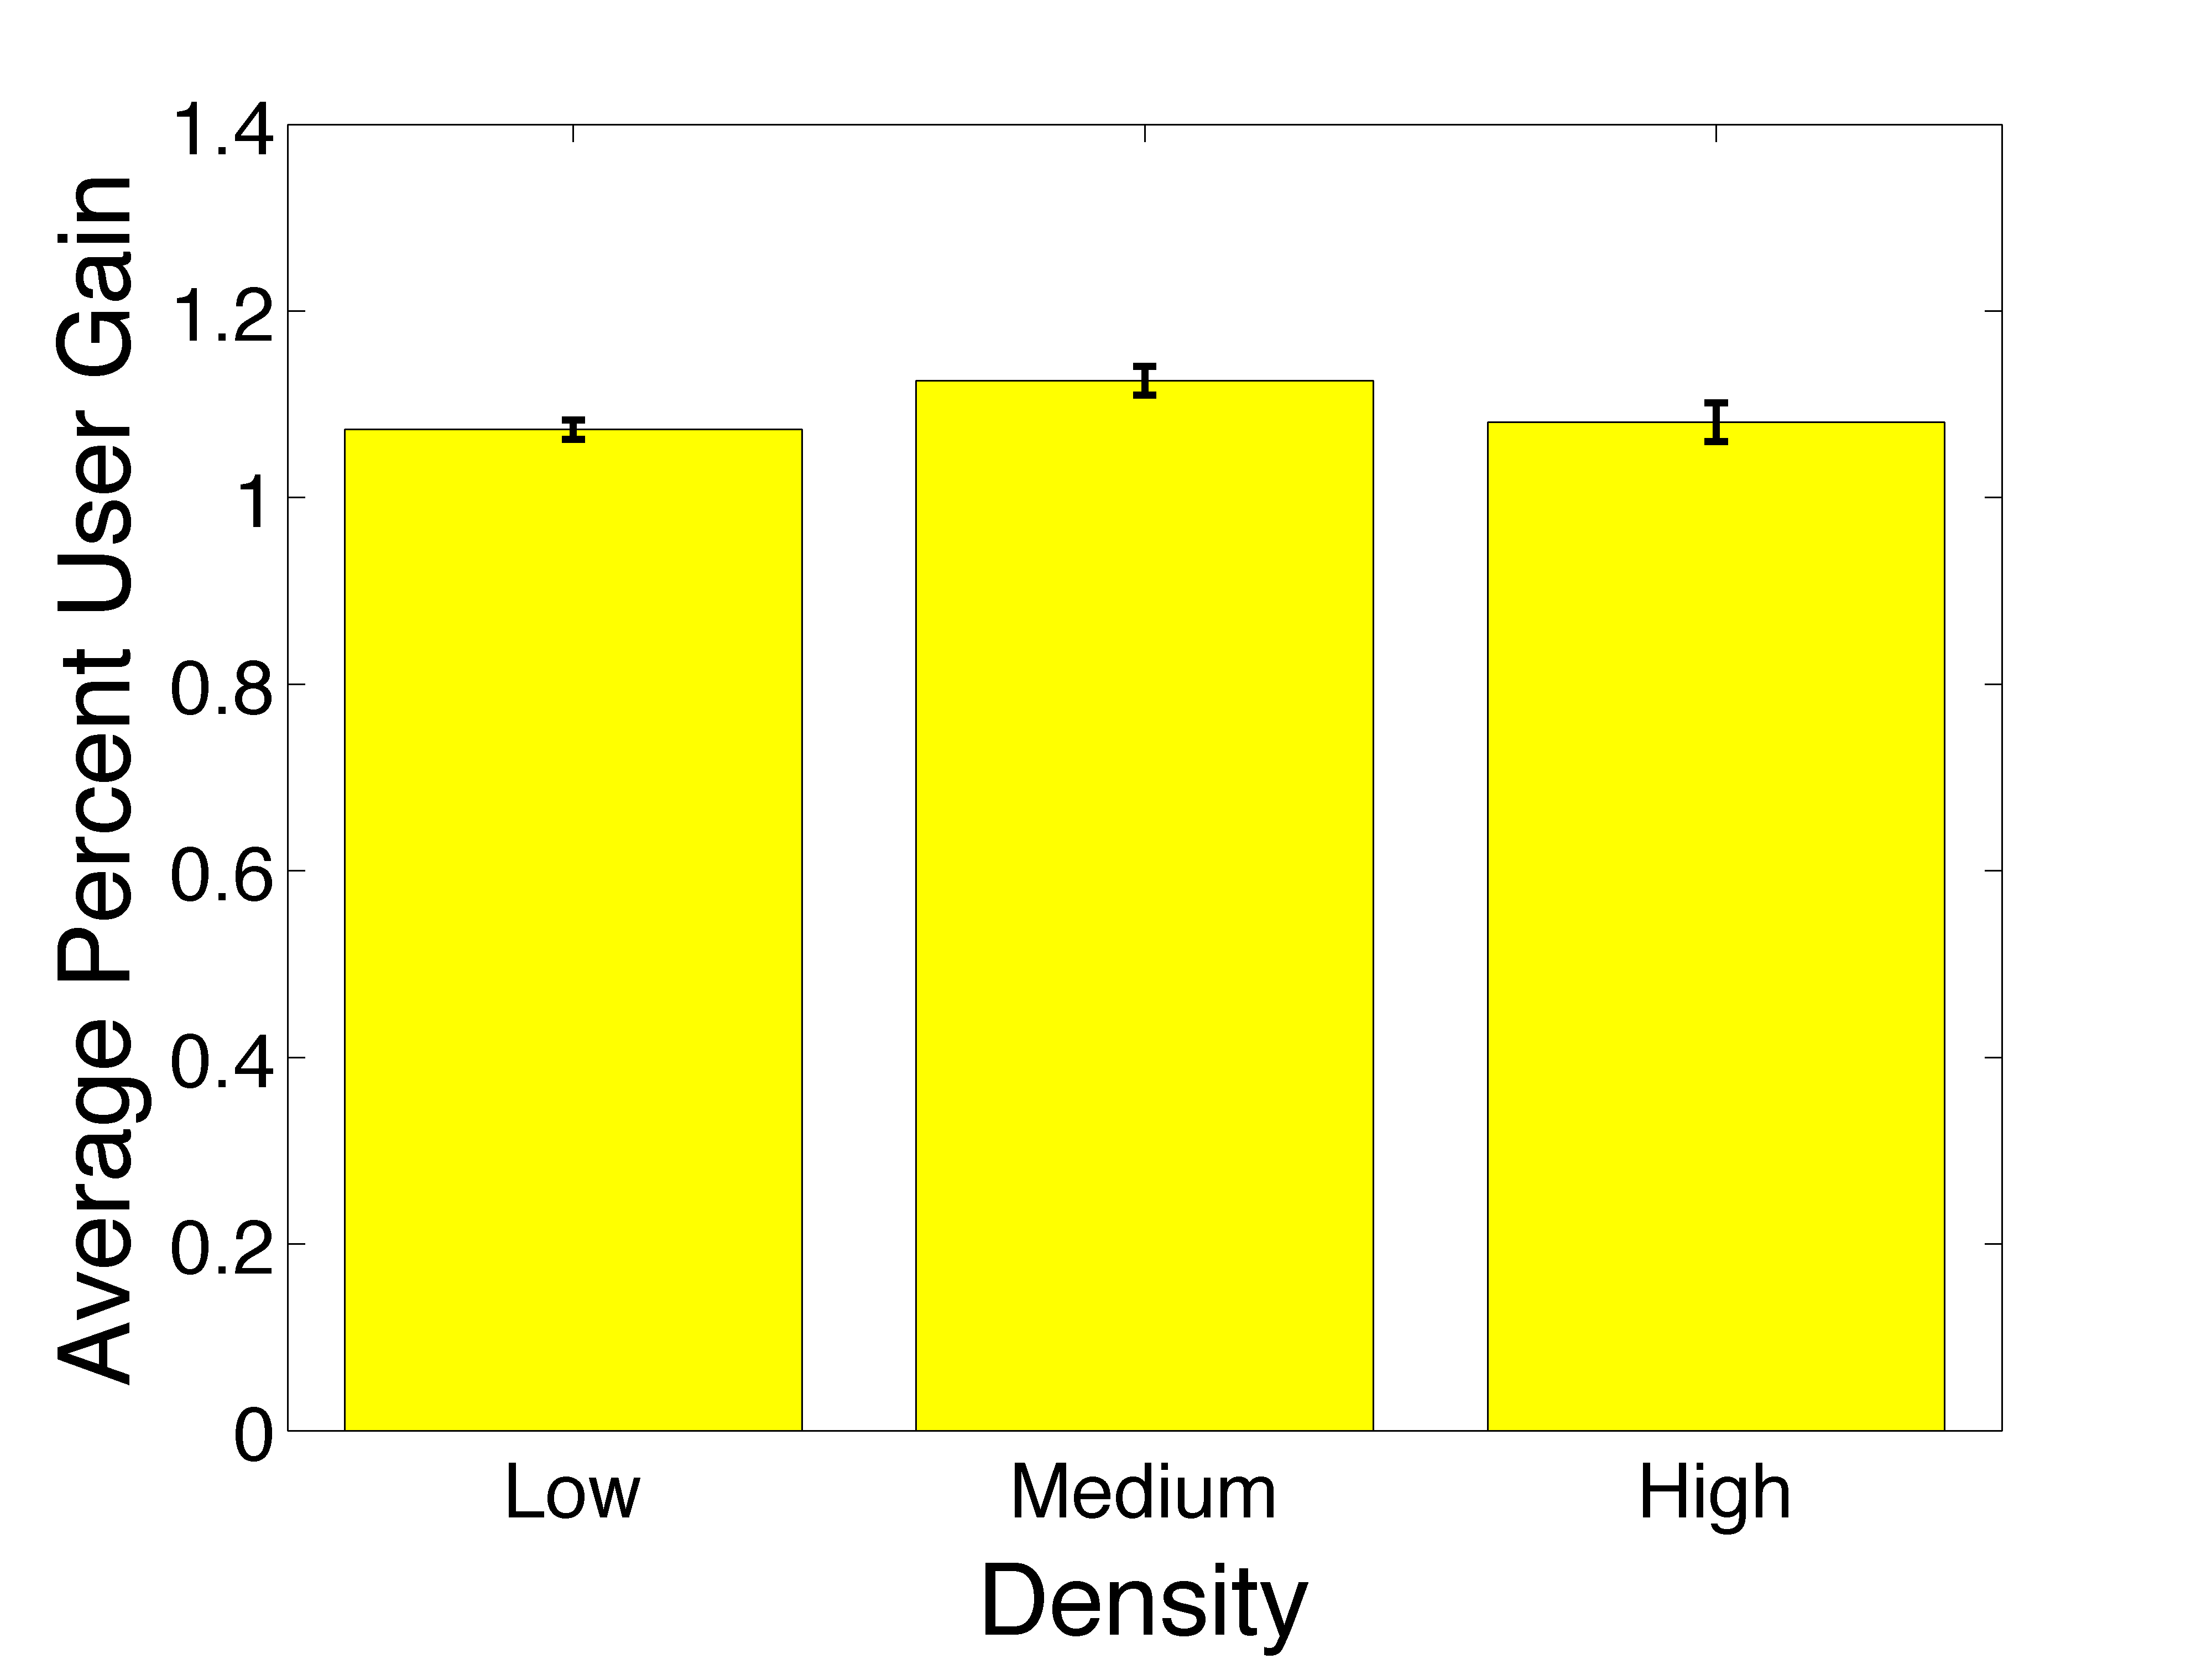
\includegraphics[width=0.32\textwidth,type=png,ext=.png,read=.png]{graphs/Random-0.875-AUG-PER}
	}
  \hspace{-0.1in}\subfigure[Scale Free $M_2$]{
	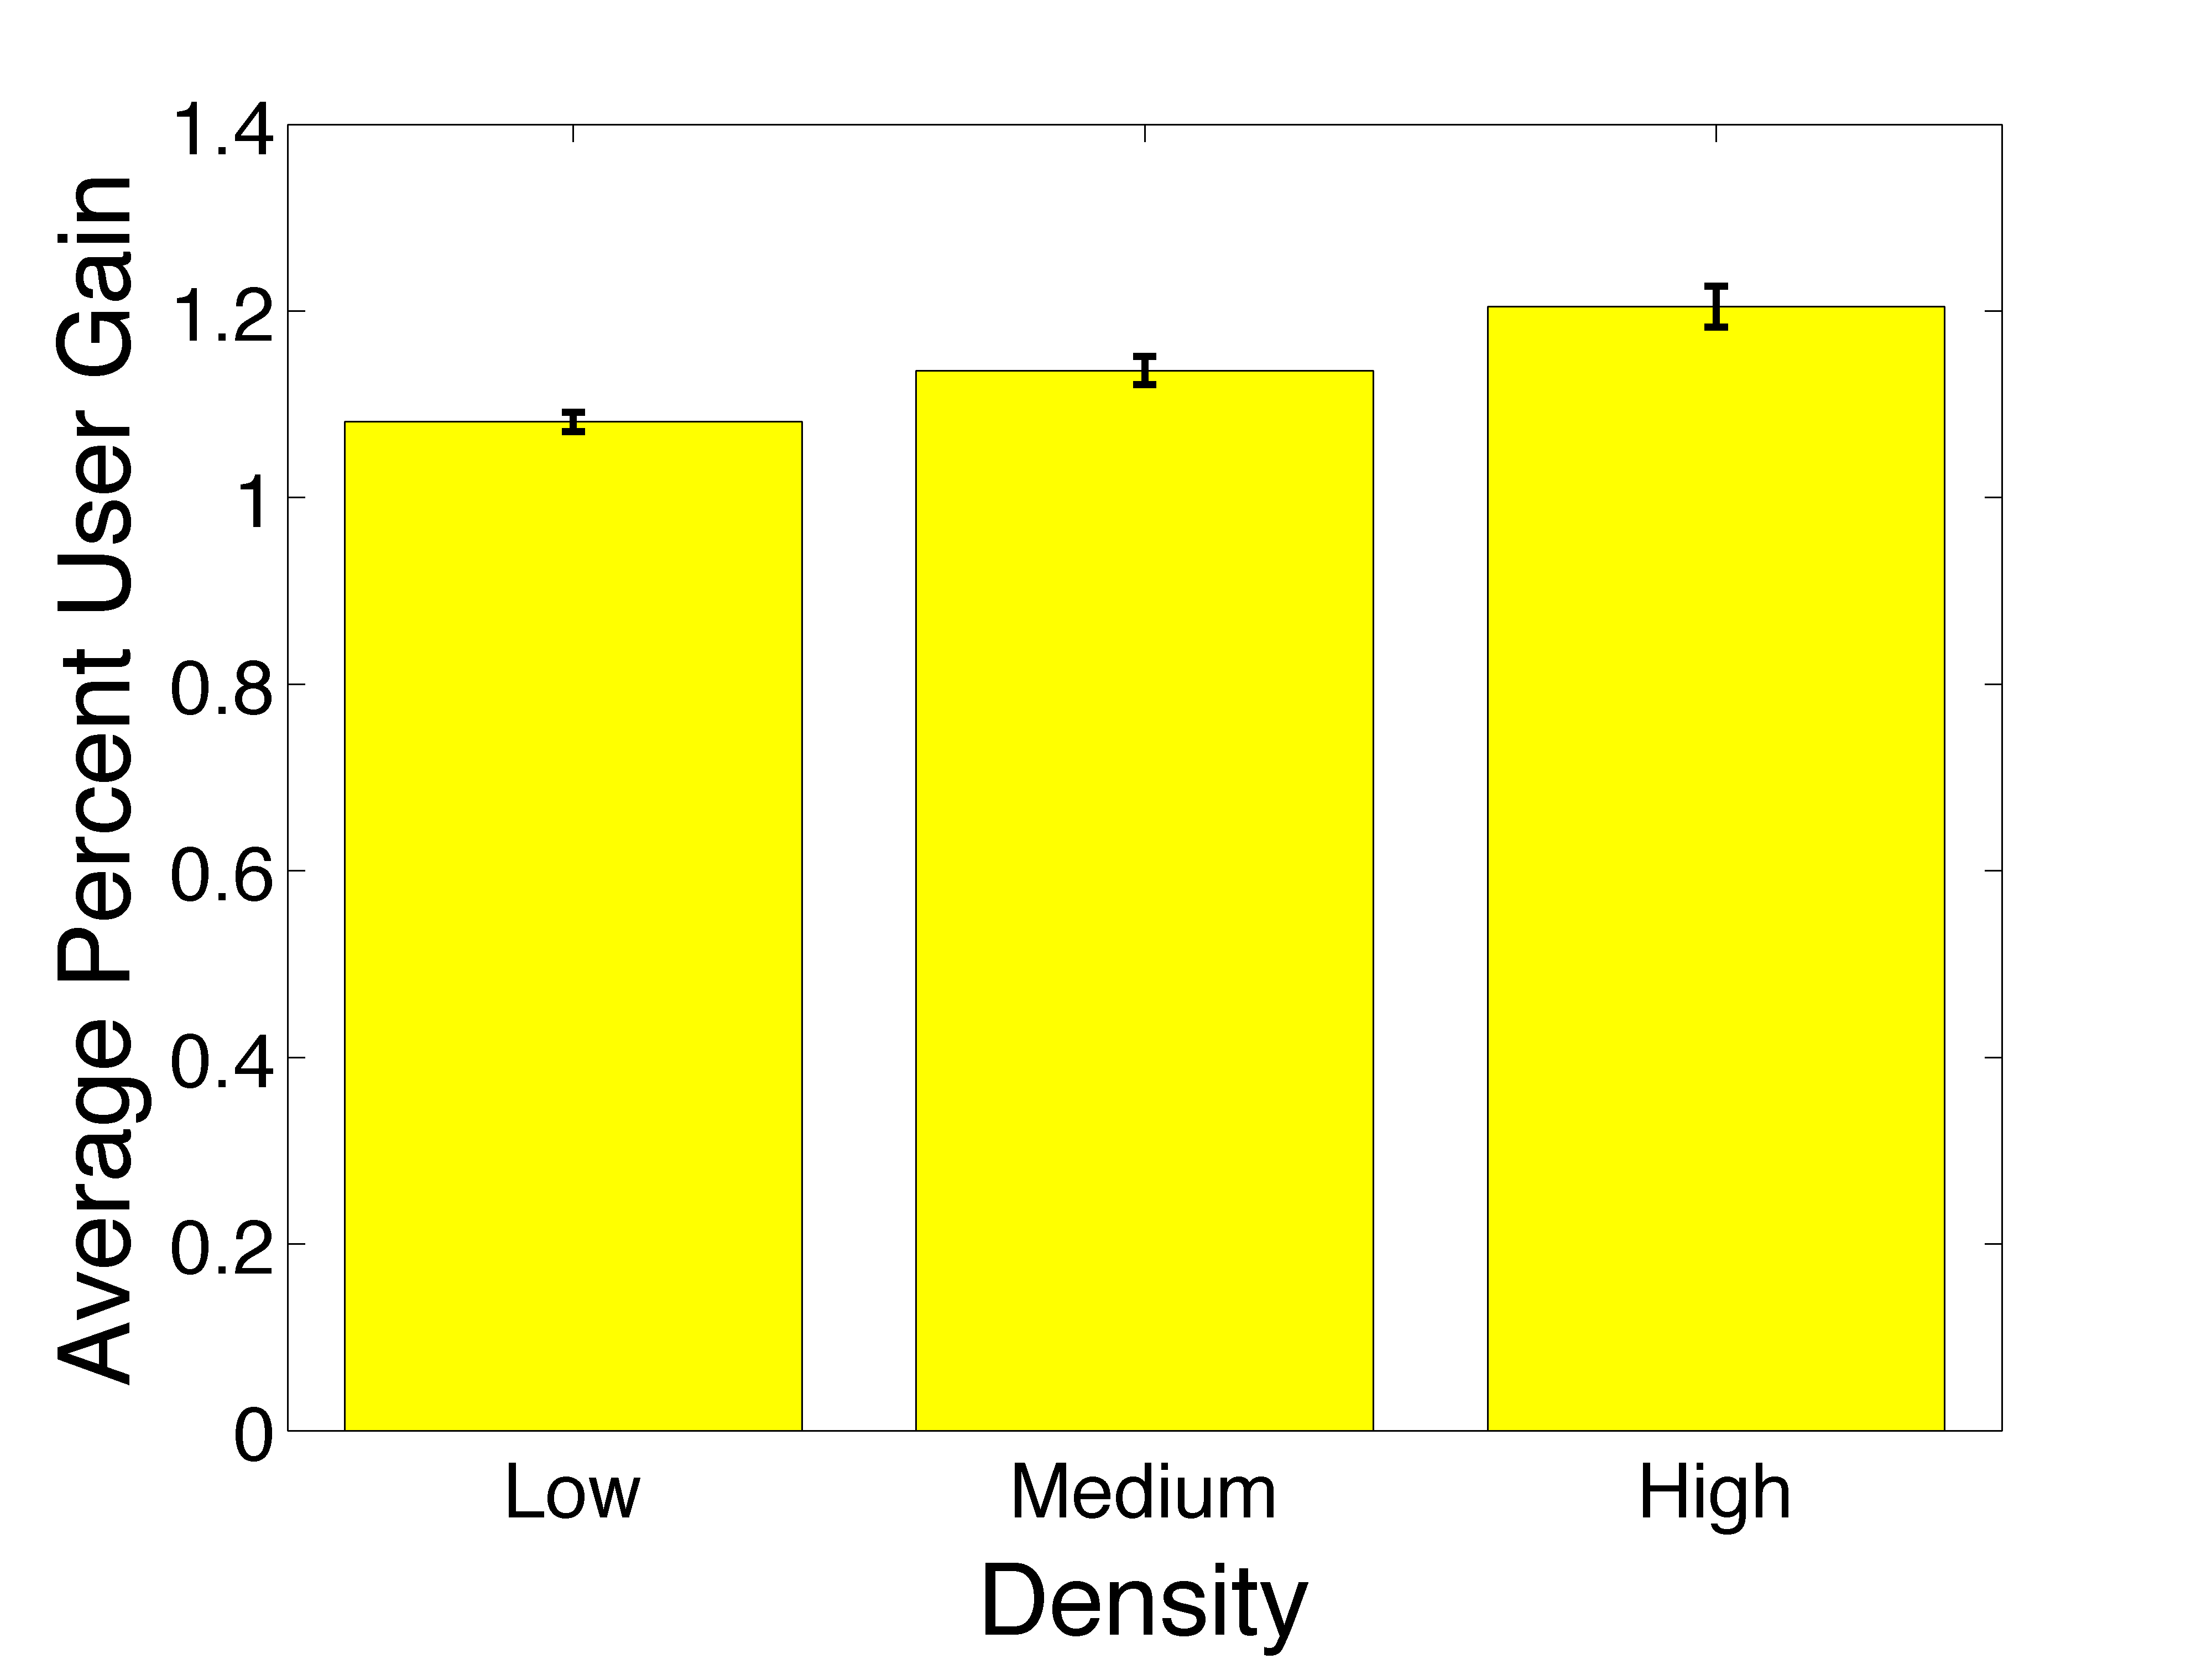
\includegraphics[width=0.32\textwidth,type=png,ext=.png,read=.png]{graphs/ScaleFree-0.875-AUG-PER}
	} 
  \hspace{-0.1in}\subfigure[Small World $M_2$]{
	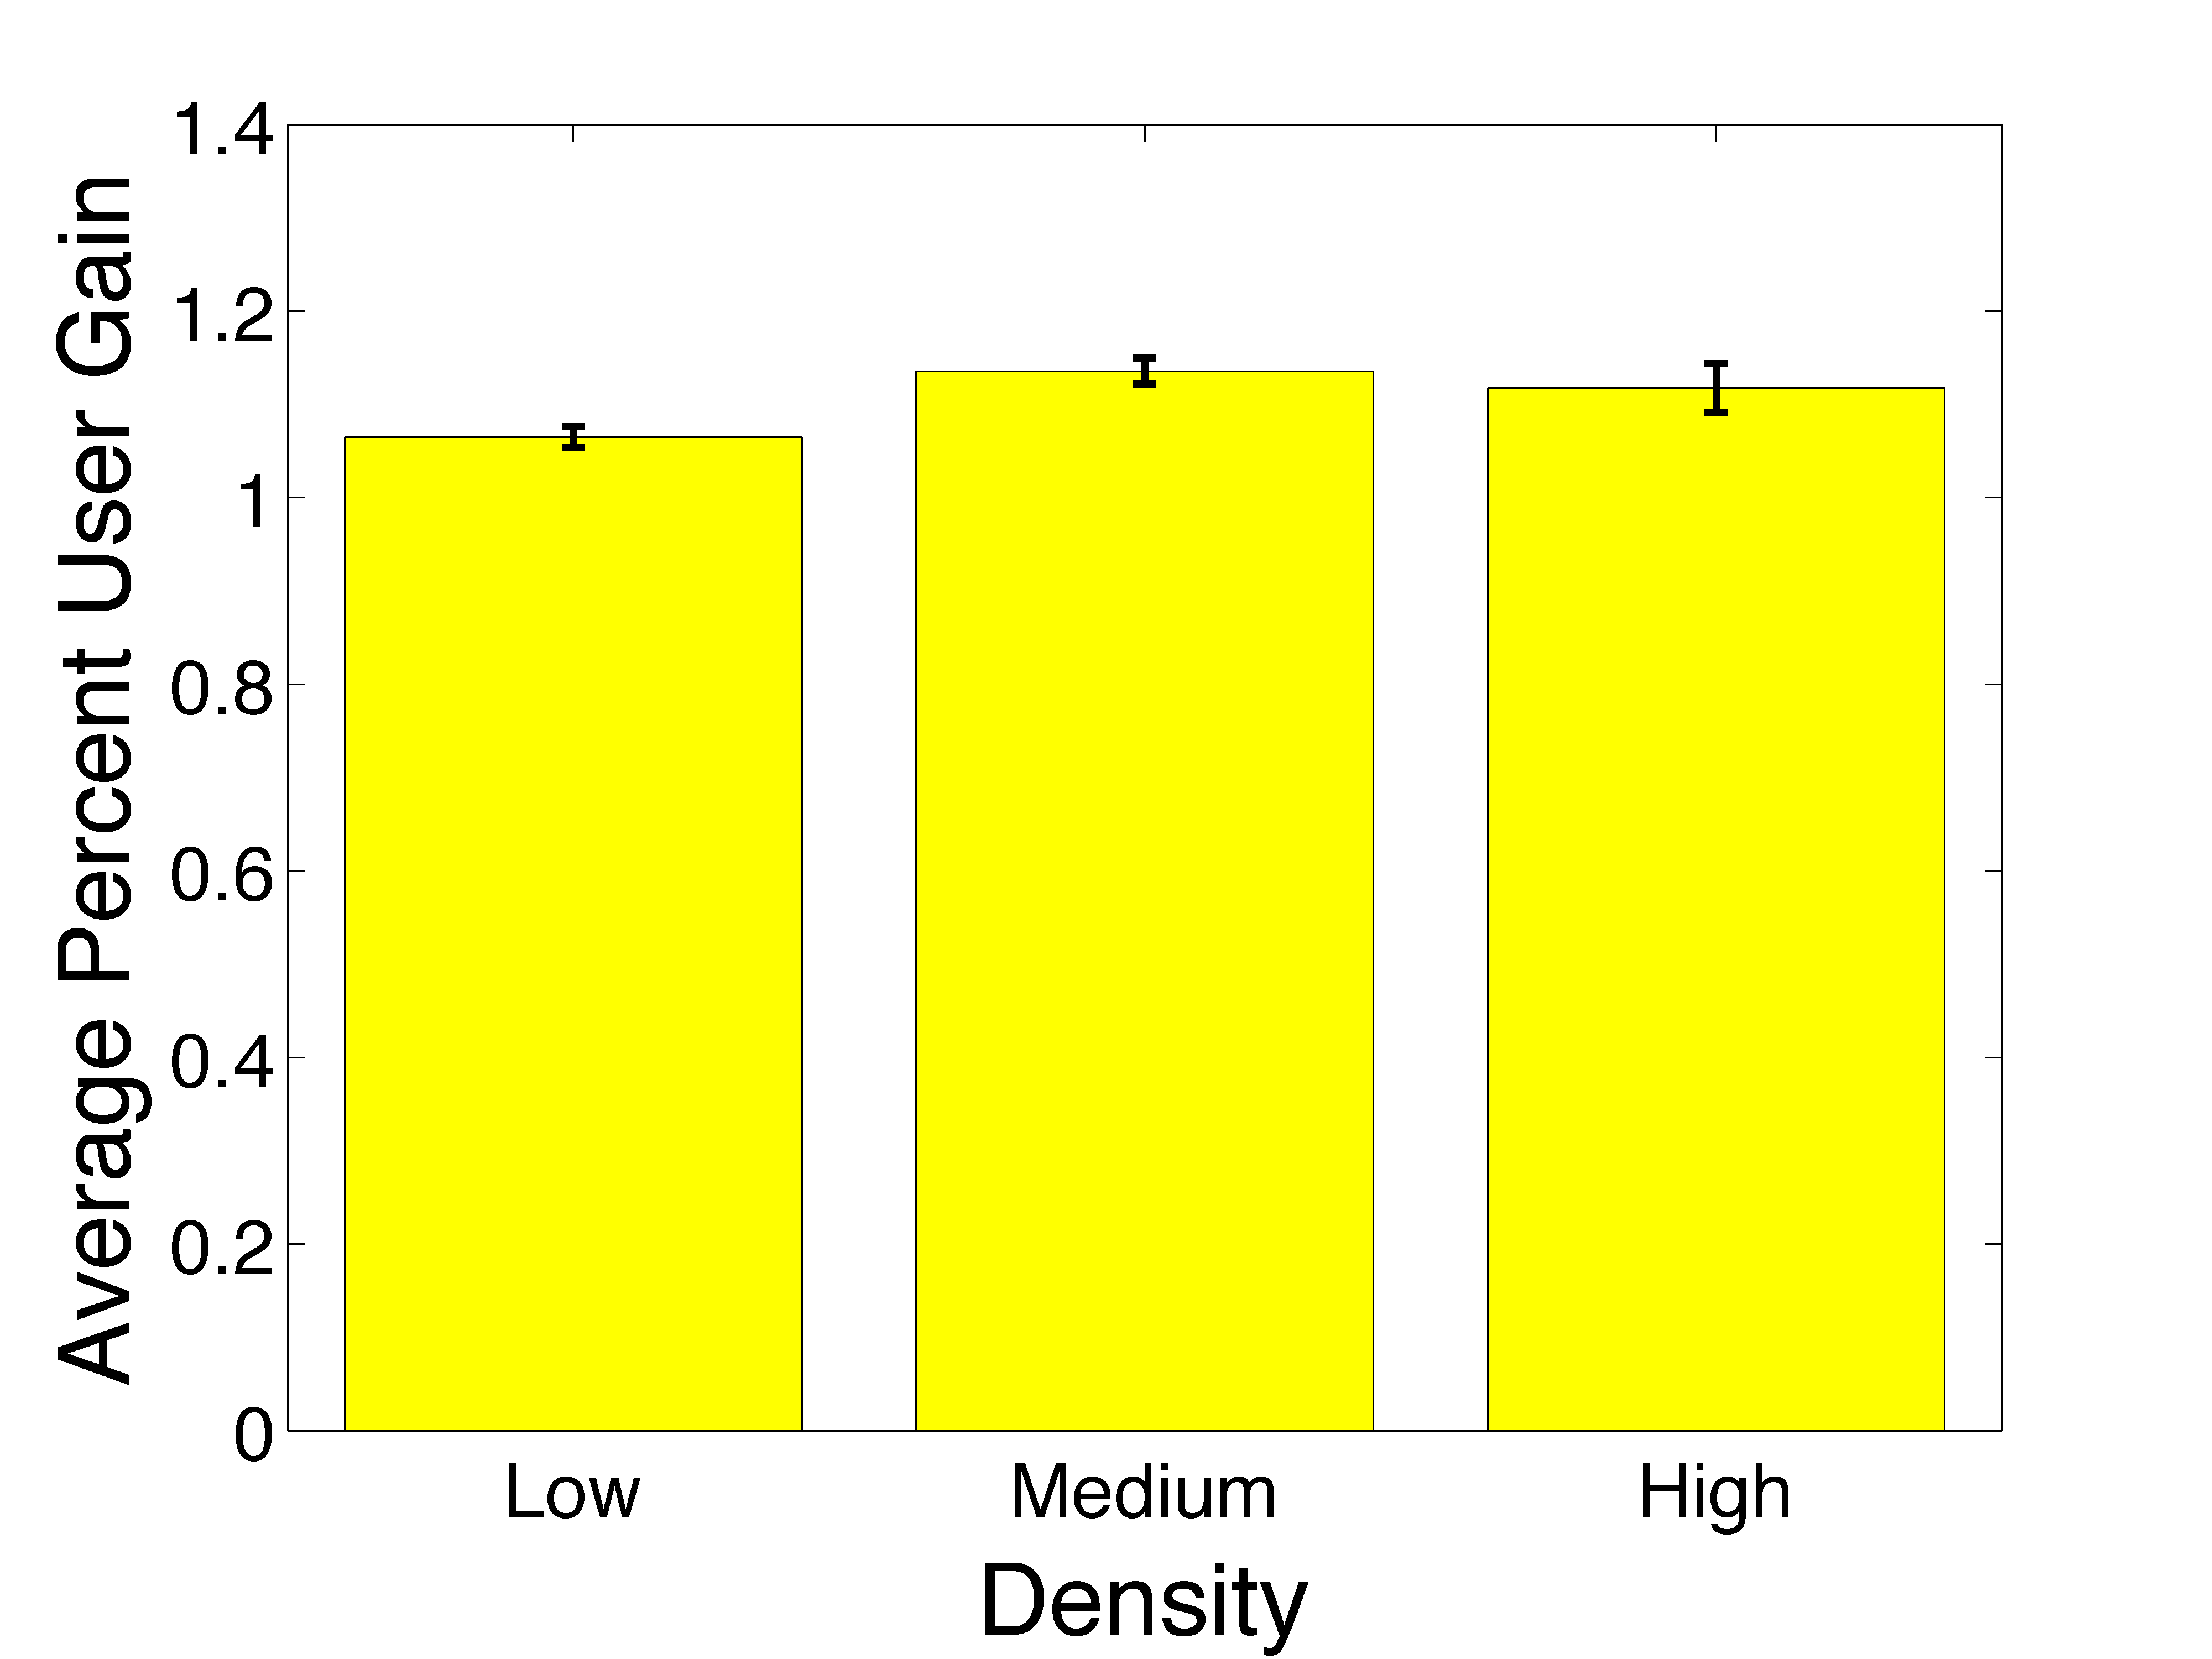
\includegraphics[width=0.32\textwidth,type=png,ext=.png,read=.png]{graphs/SmallWorld-0.875-AUG-PER}
	}
	
   \hspace{-0.1in}\subfigure[Random Graphs $M_3$]{
	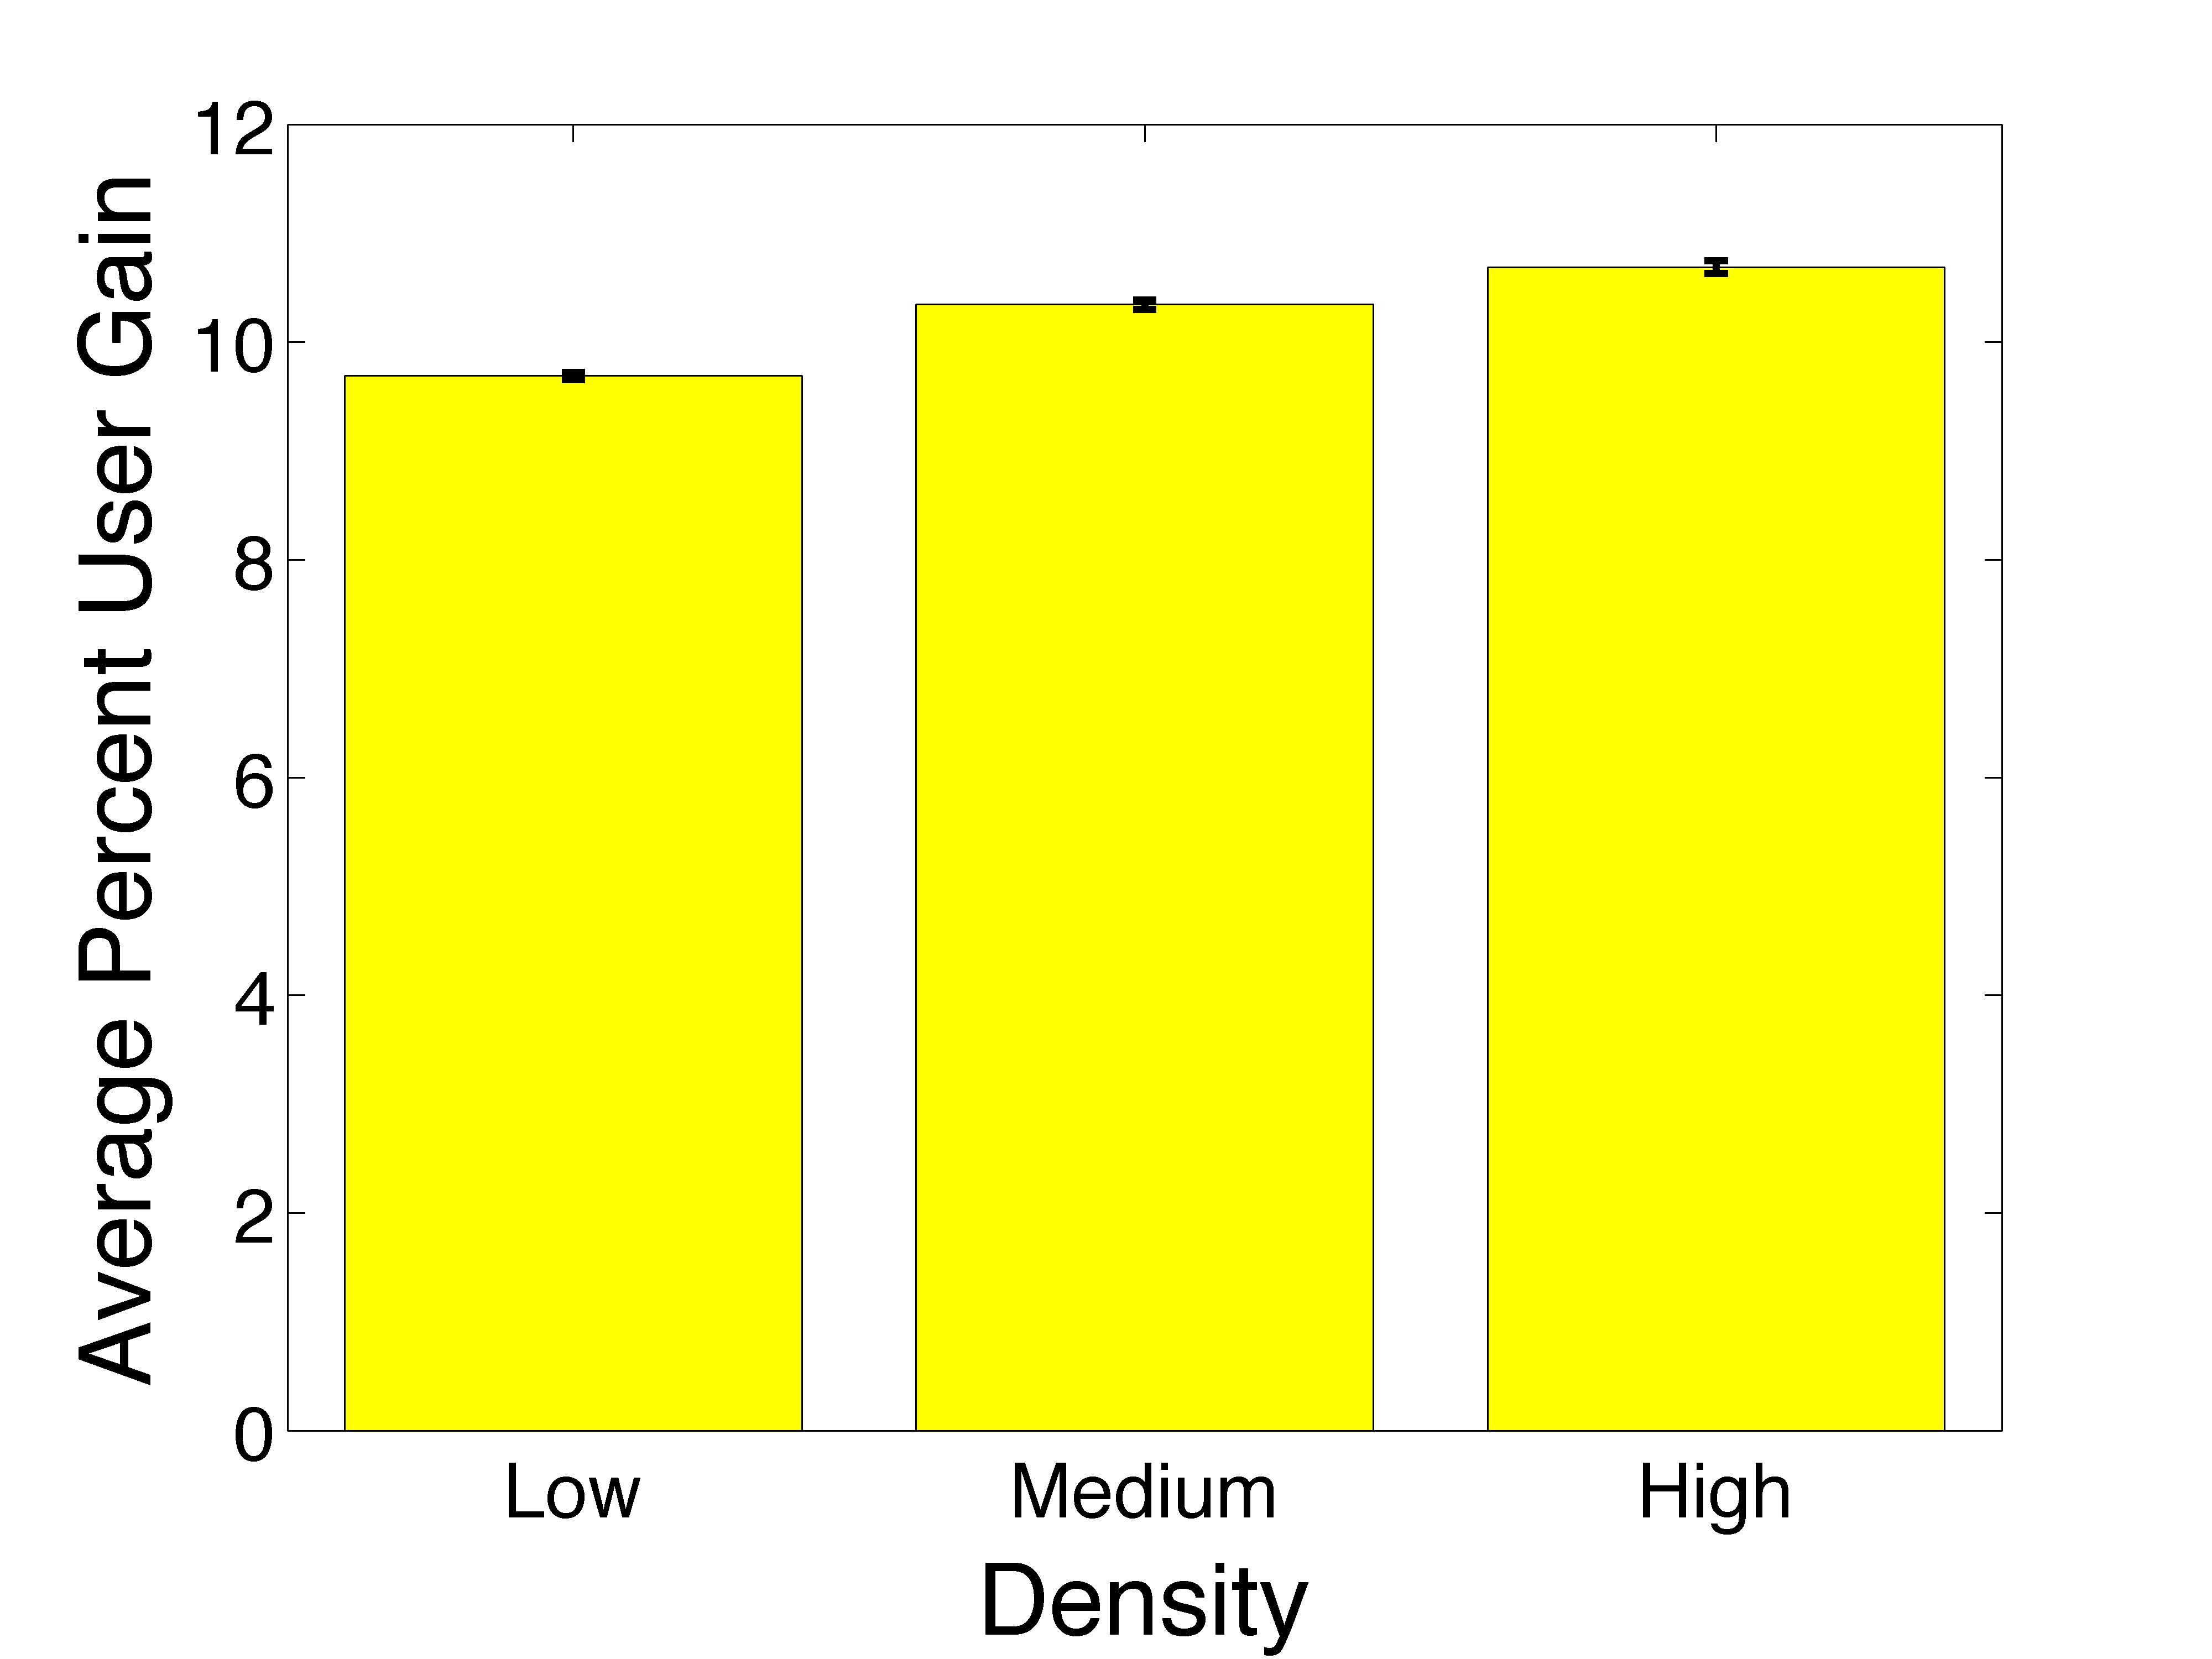
\includegraphics[width=0.32\textwidth,type=png,ext=.png,read=.png]{graphs/Random-0.500-AUG-PER}
	}  
  \hspace{-0.1in}\subfigure[Scale Free $M_3$]{
	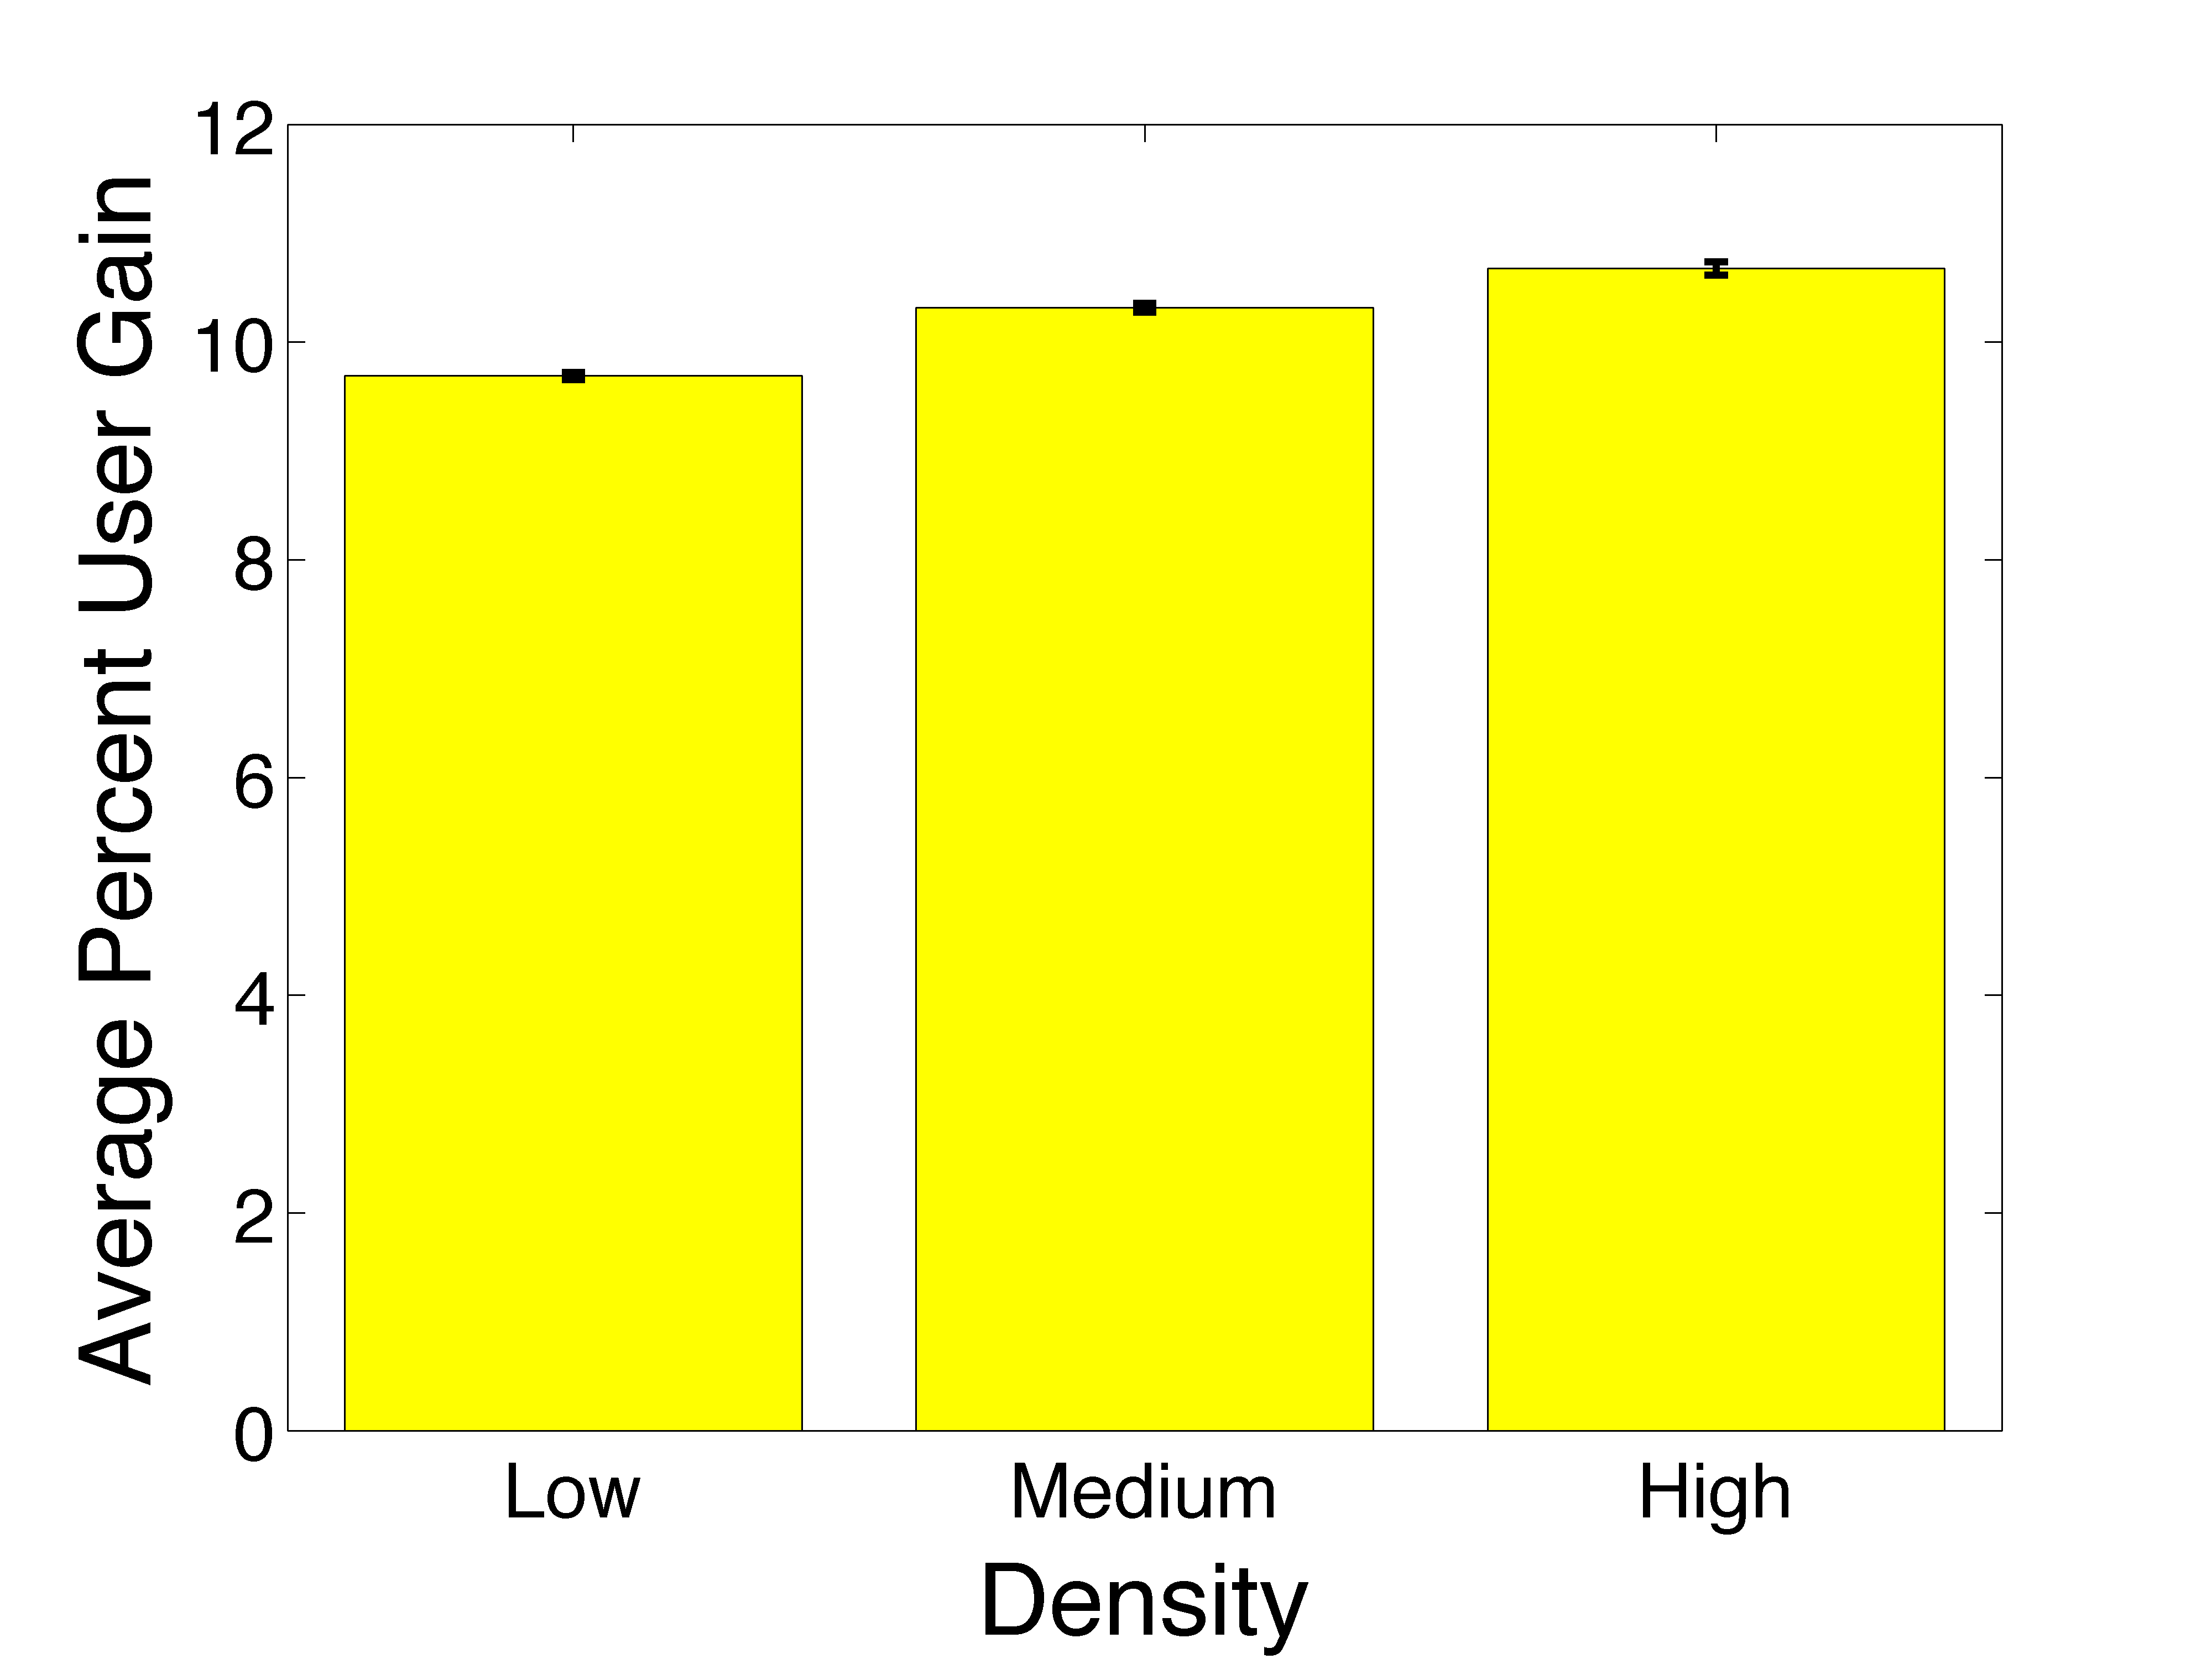
\includegraphics[width=0.32\textwidth,type=png,ext=.png,read=.png]{graphs/ScaleFree-0.500-AUG-PER}
	}  
  \hspace{-0.1in}\subfigure[Small World $M_3$]{
	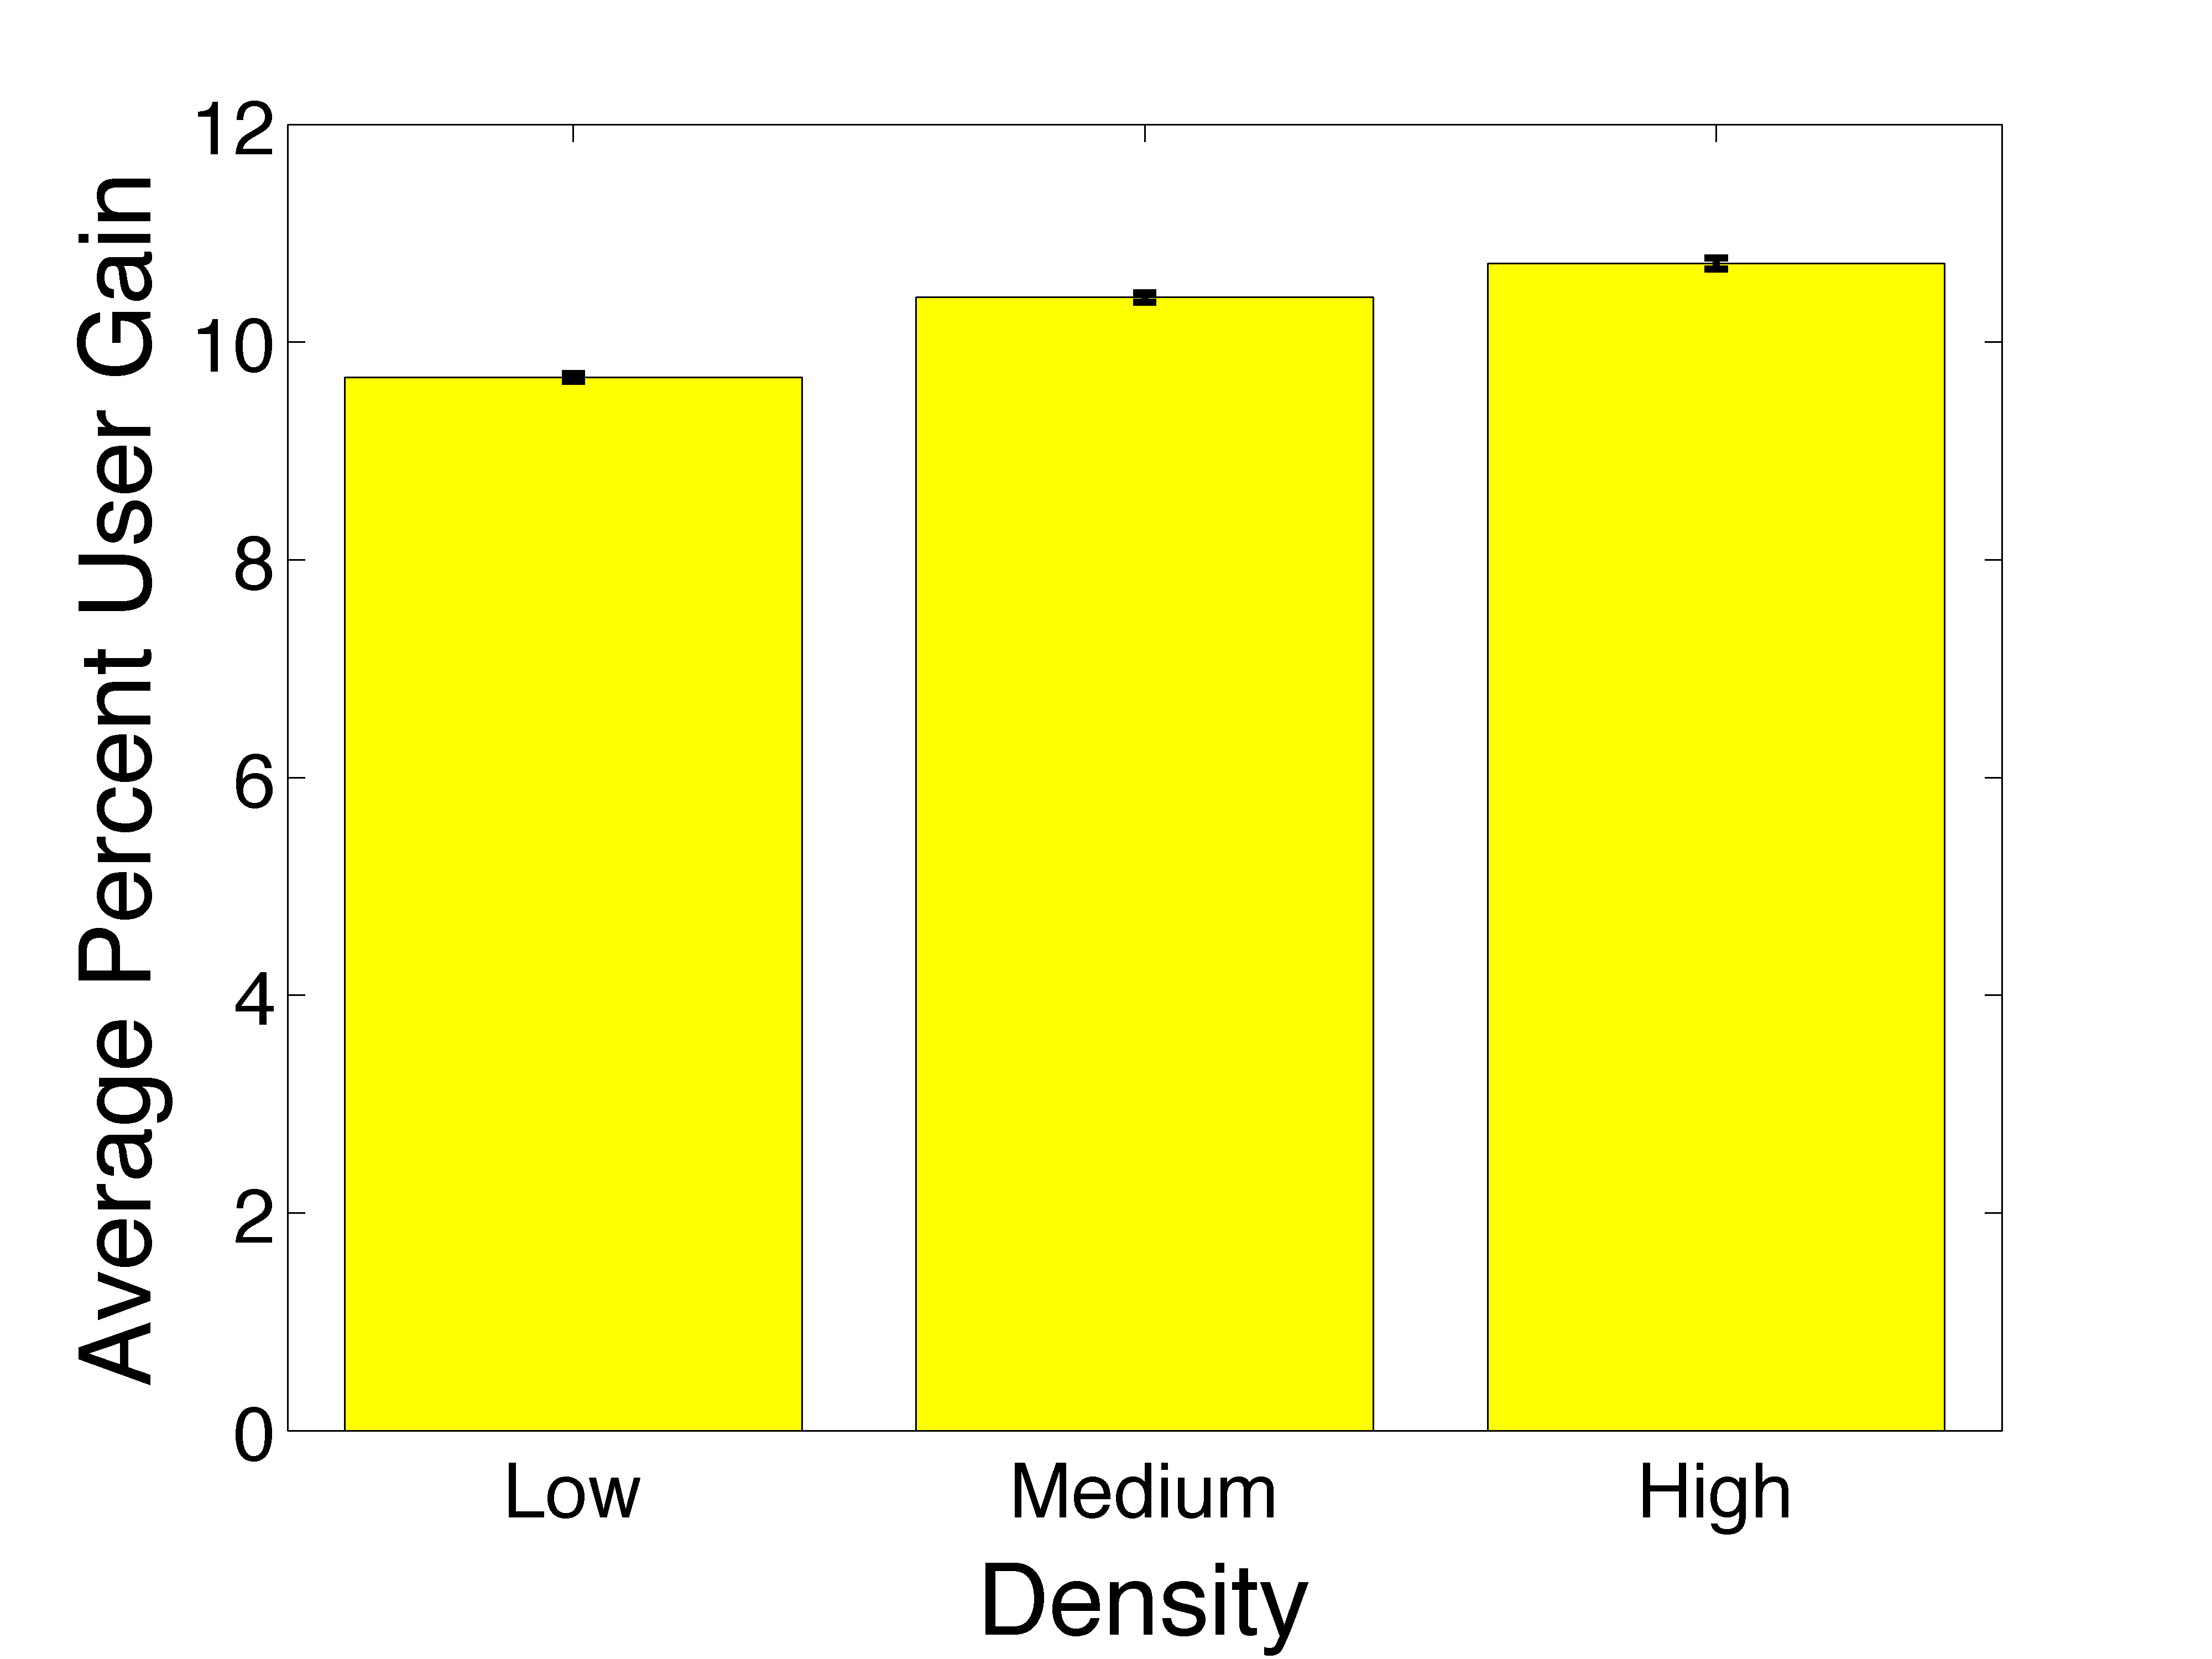
\includegraphics[width=0.32\textwidth,type=png,ext=.png,read=.png]{graphs/SmallWorld-0.500-AUG-PER}
	}   
  \caption{Graphs showing the average percent gain of consumers on
  different topologies and densities under market conditions $M_1$ (a)-(c), $M_2$ (d)-(f) and $M_3$ (g)-(i).}
  \label{fig:graphs_gain}
\end{figure*}

\begin{figure*}
  \centering
  \hspace{-0.1in}\subfigure[Random Graphs $M_1$]{
  	%\label{fig:res_walsh_bandwidth}
	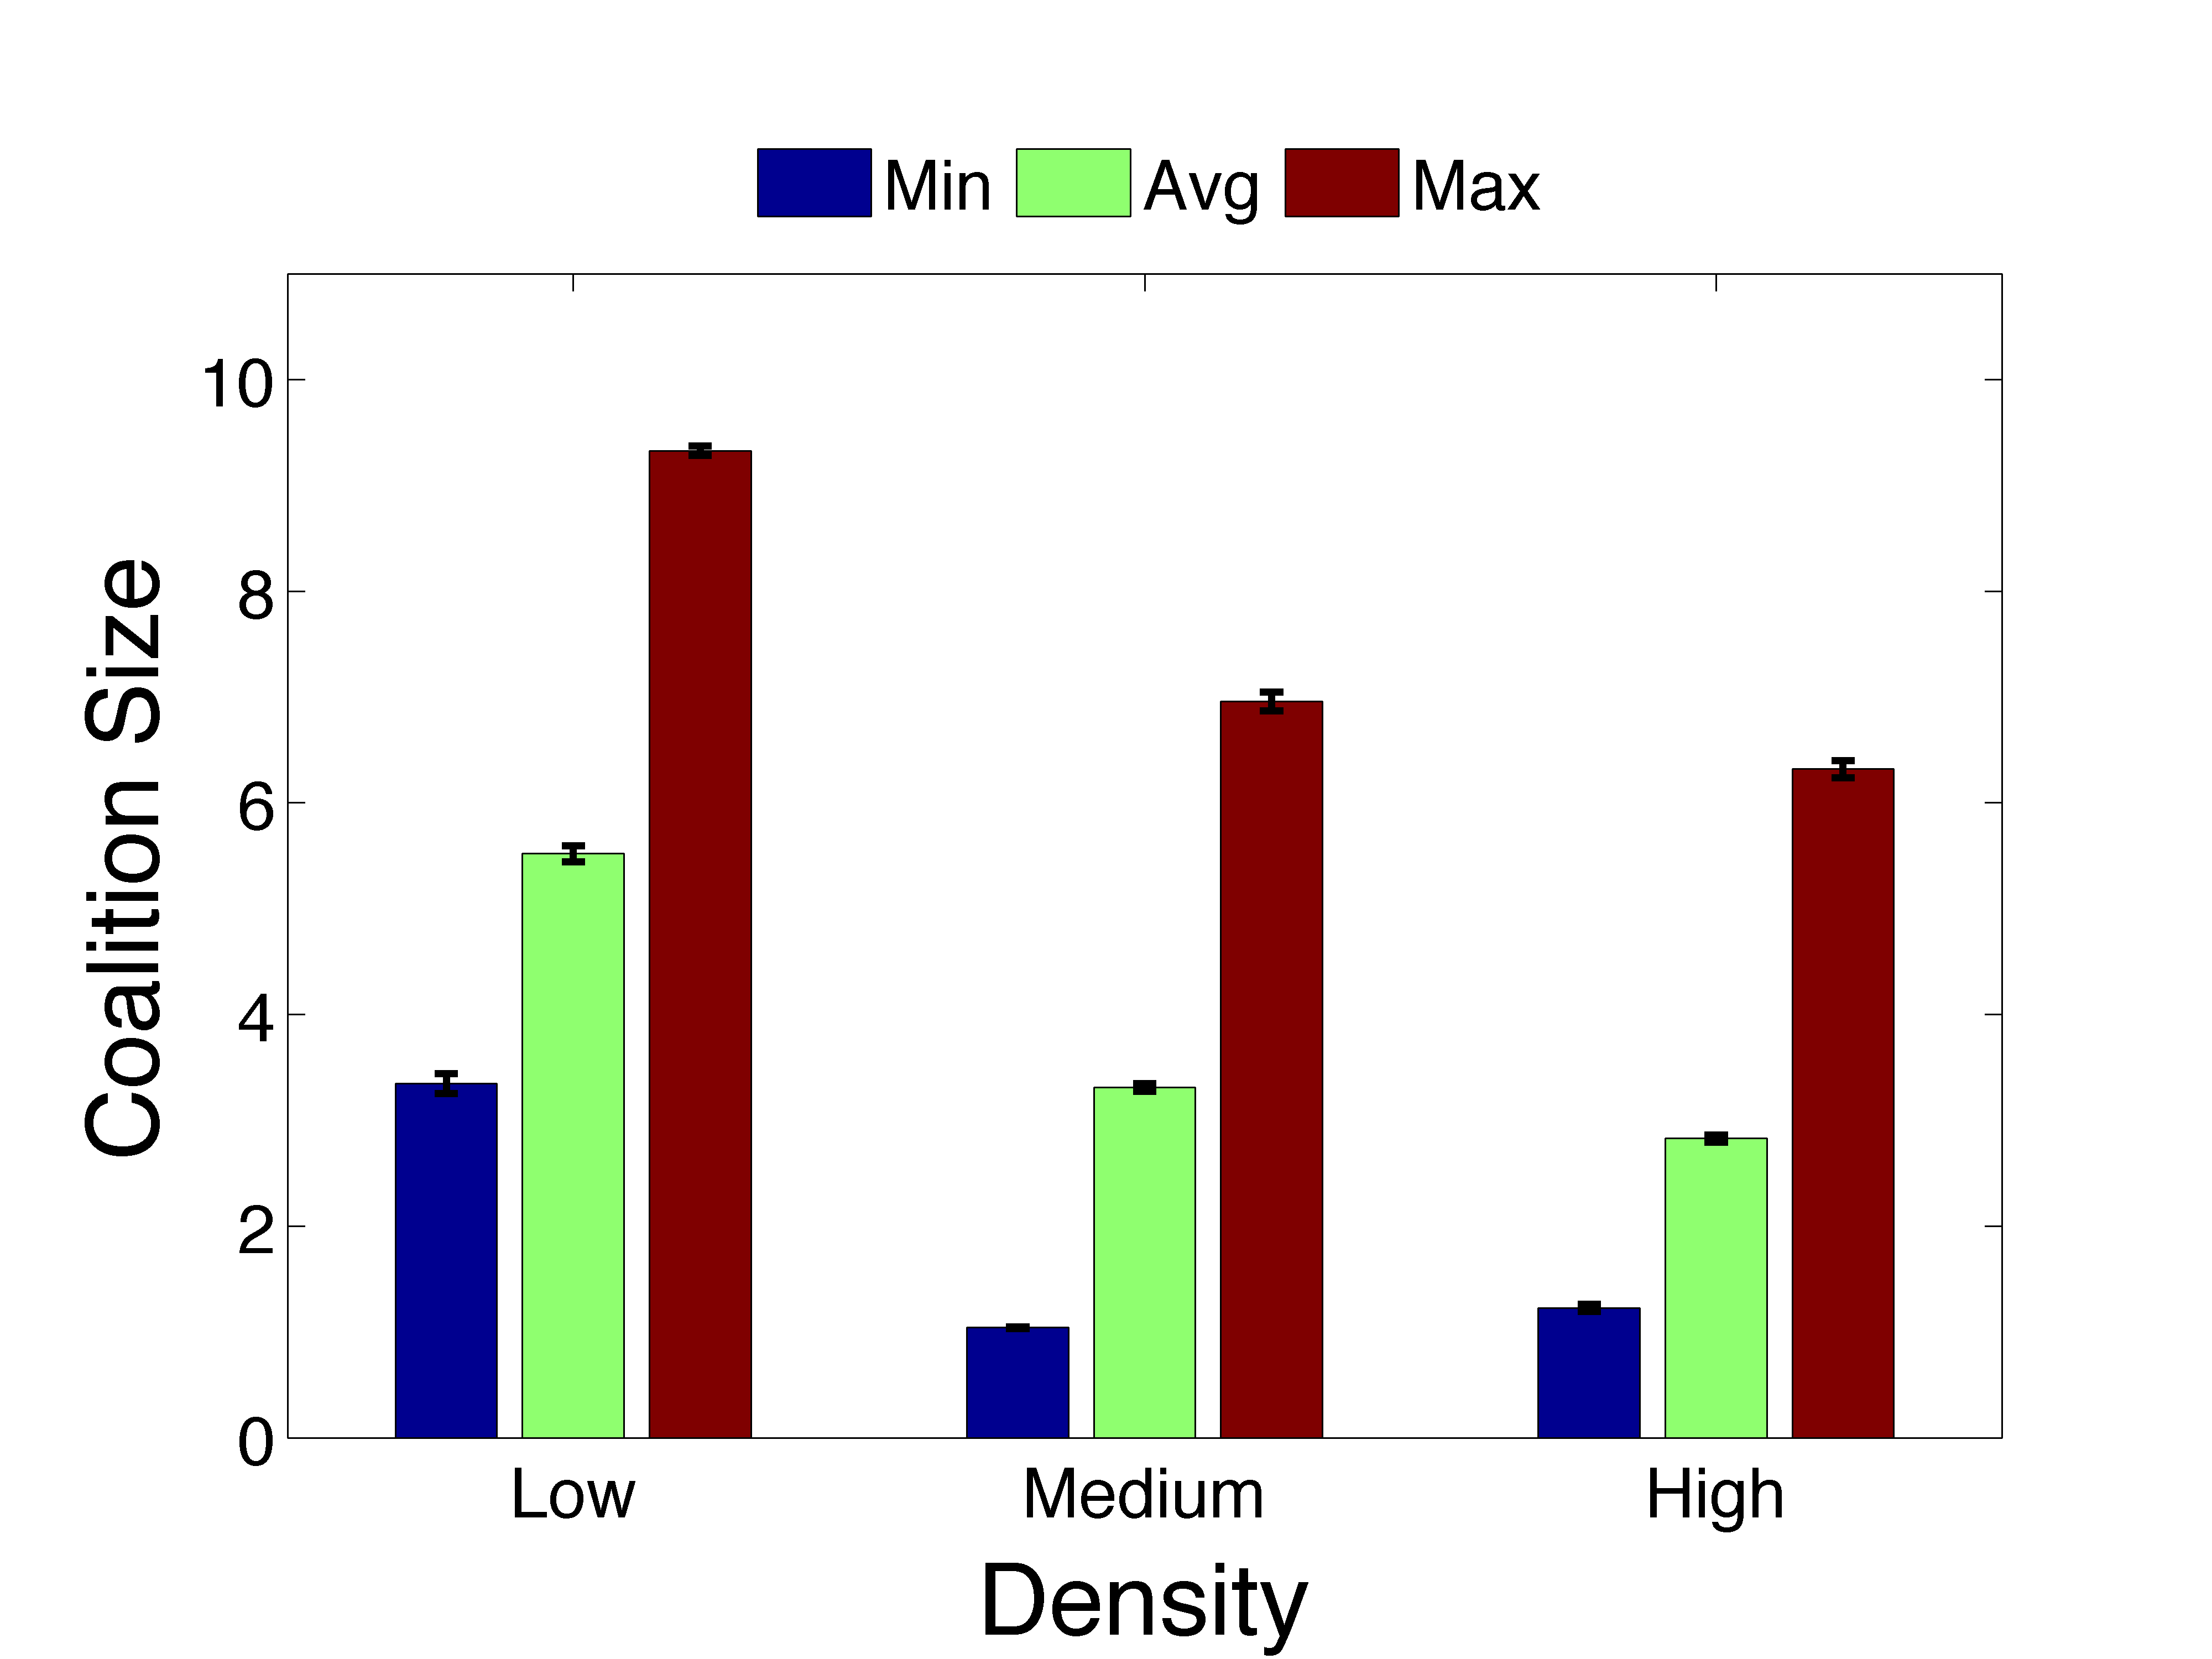
\includegraphics[width=0.49\textwidth,type=png,ext=.png,read=.png]{graphs/Random-1.000-Size}
	}
  \hspace{-0.1in}\subfigure[Random Graphs $M_2$]{
  	%\label{fig:res_walsh_bandwidth}
	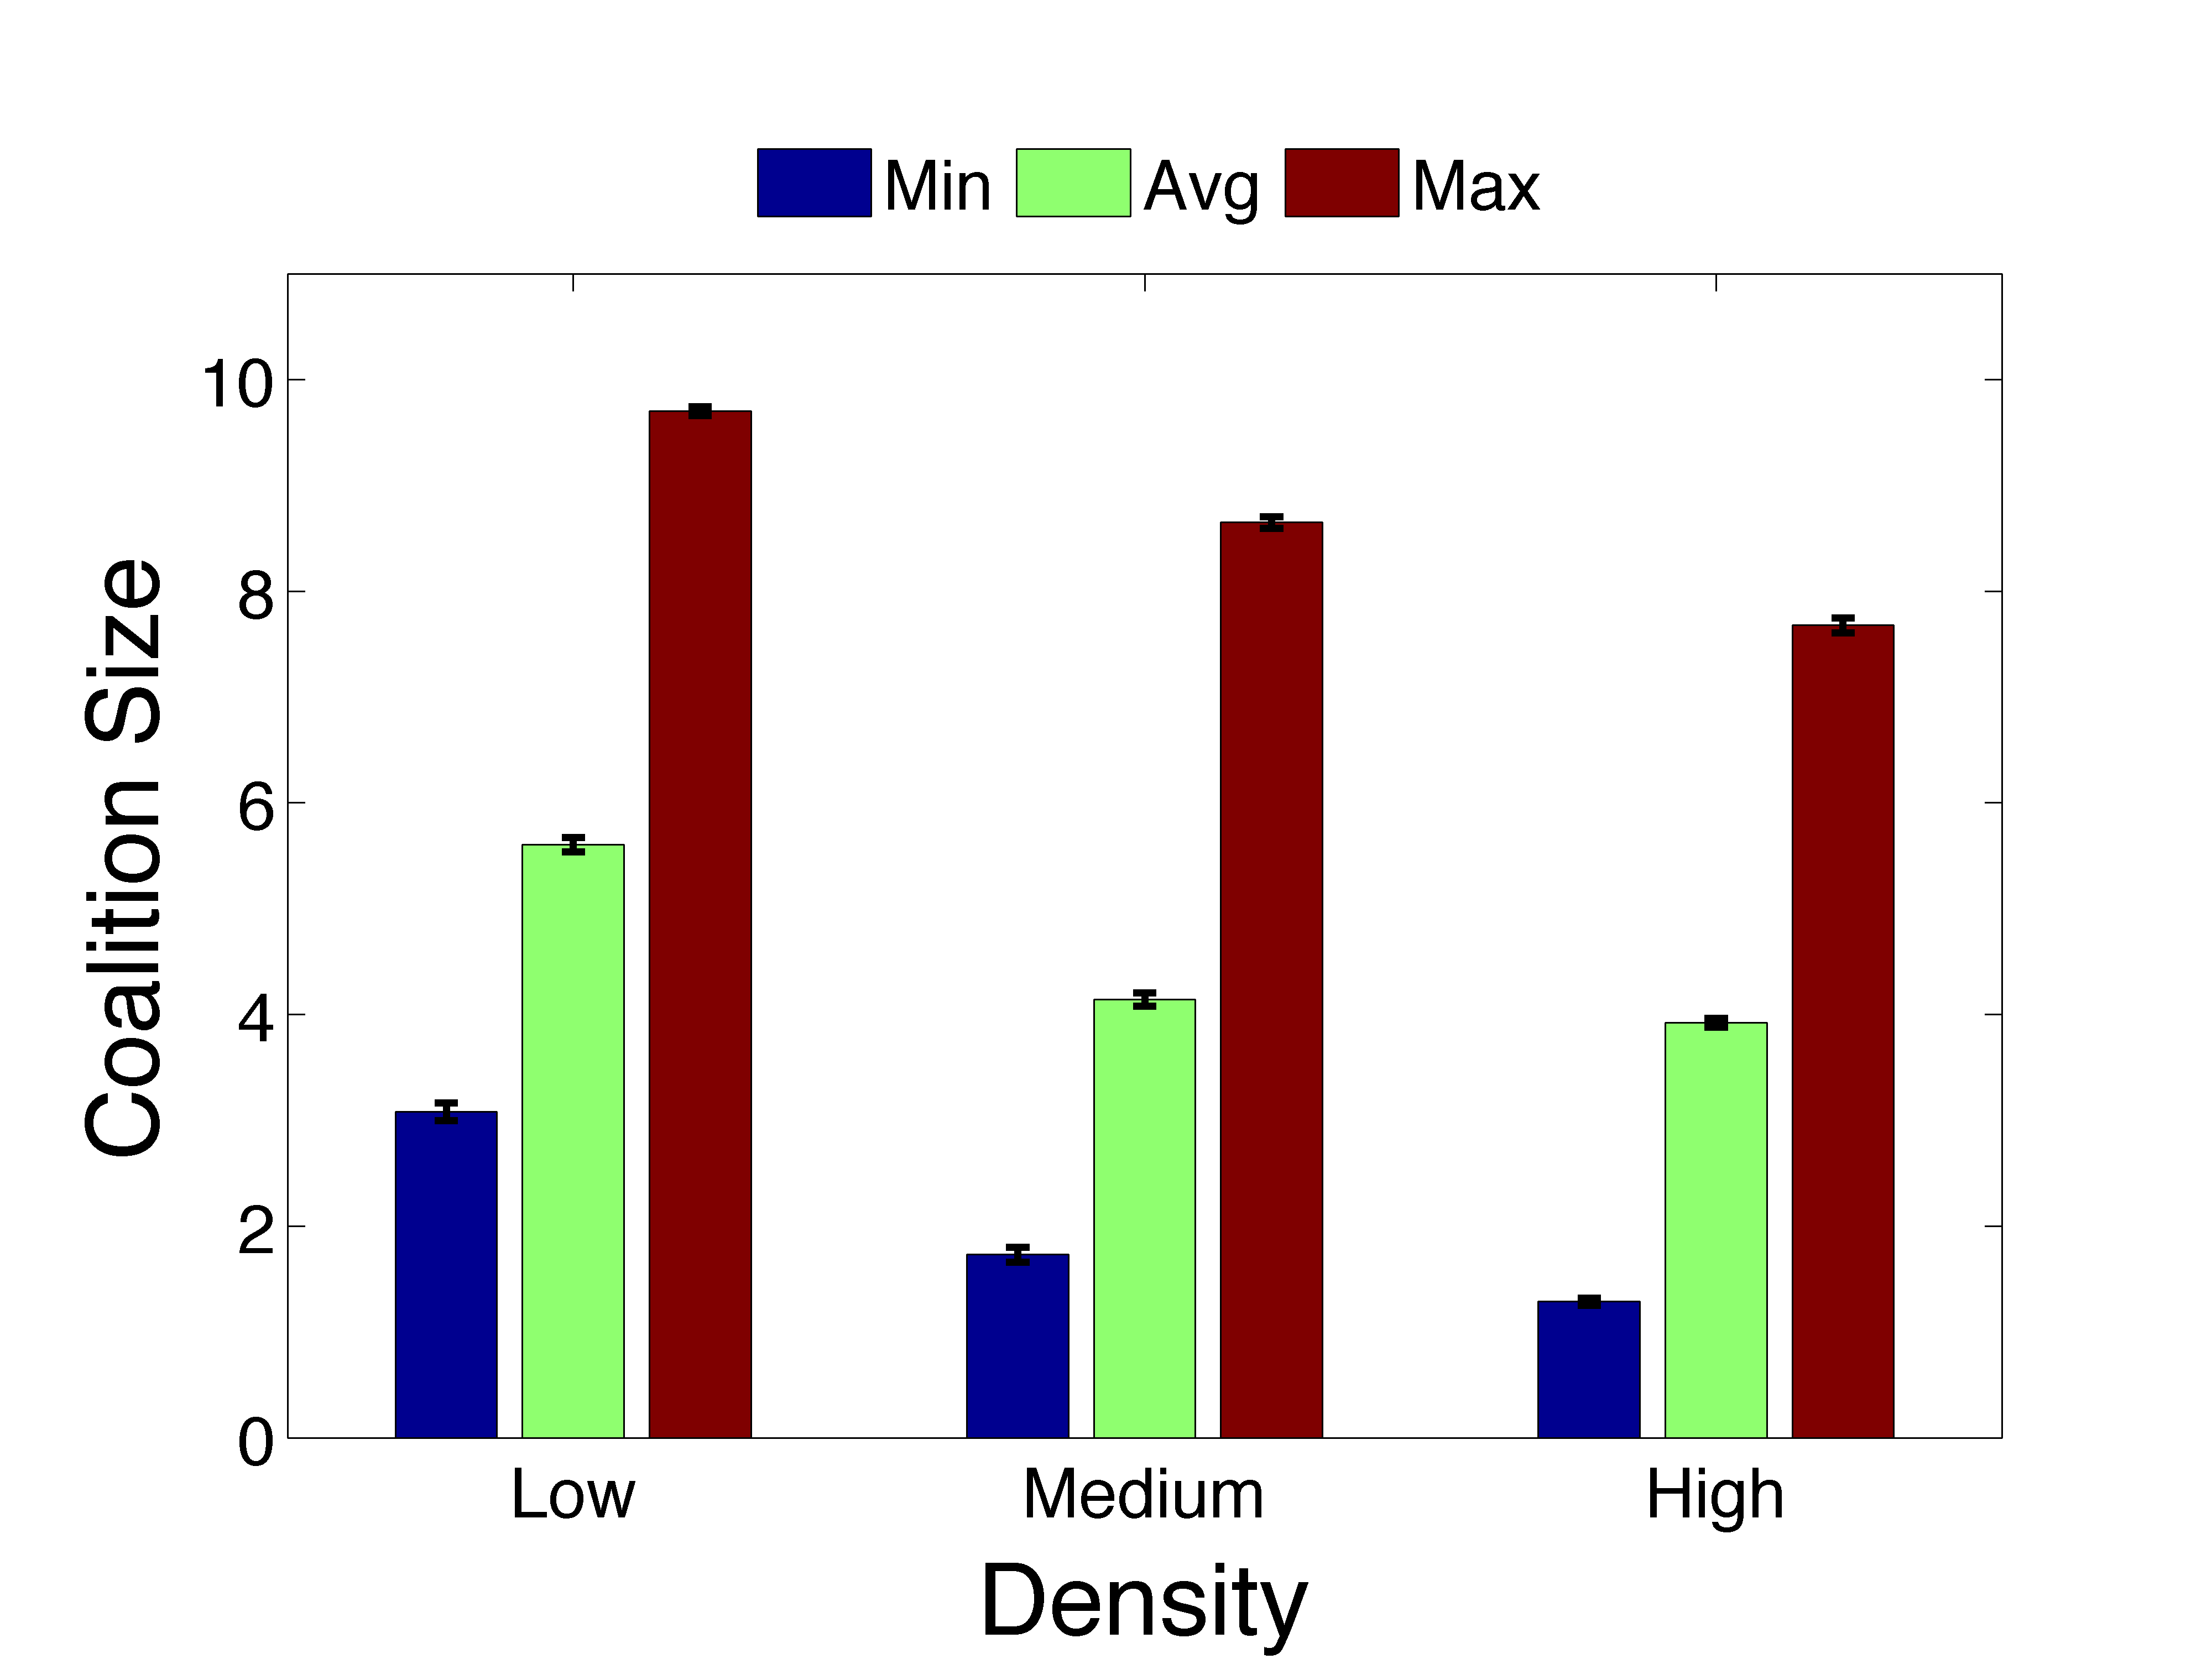
\includegraphics[width=0.49\textwidth,type=png,ext=.png,read=.png]{graphs/Random-0.875-Size}
	}
	
  \hspace{-0.1in}\subfigure[Scale Free $M_1$]{
  	%\label{fig:res_mmuca_bandwidth}
	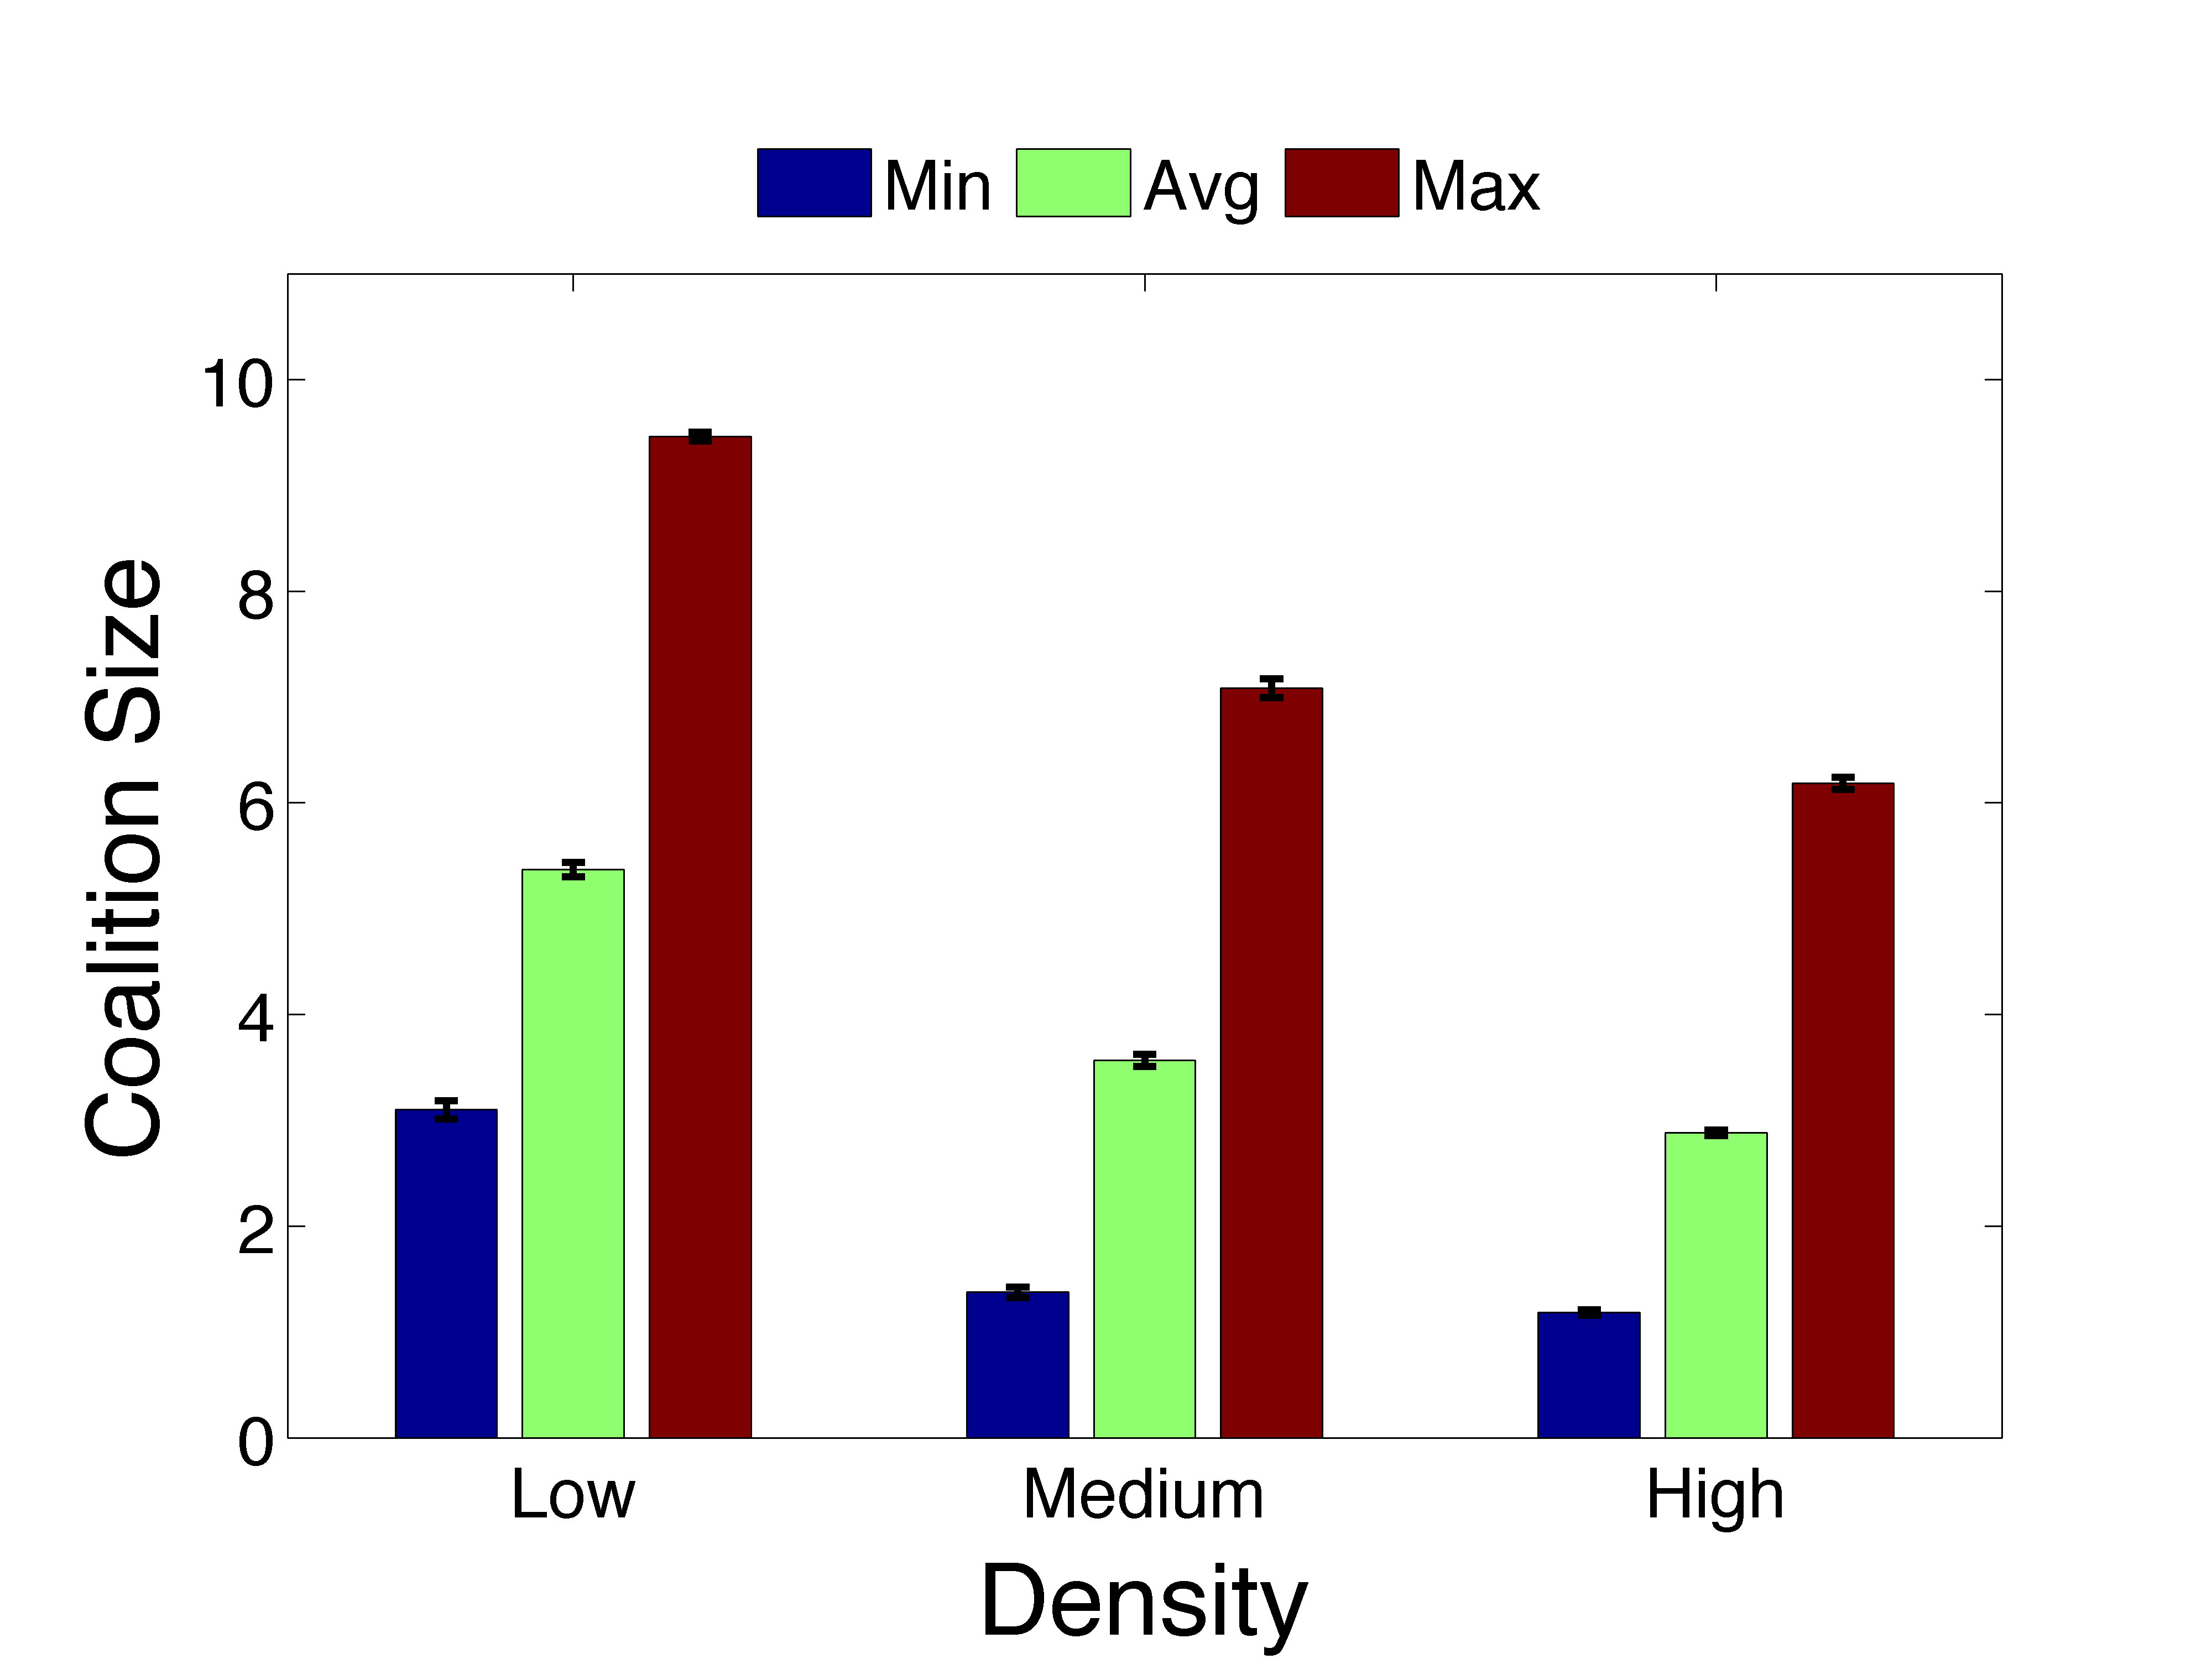
\includegraphics[width=0.49\textwidth,type=png,ext=.png,read=.png]{graphs/ScaleFree-1.000-Size}
	}
  \hspace{-0.1in}\subfigure[Scale Free $M_2$]{
  	%\label{fig:res_mmuca_bandwidth}
	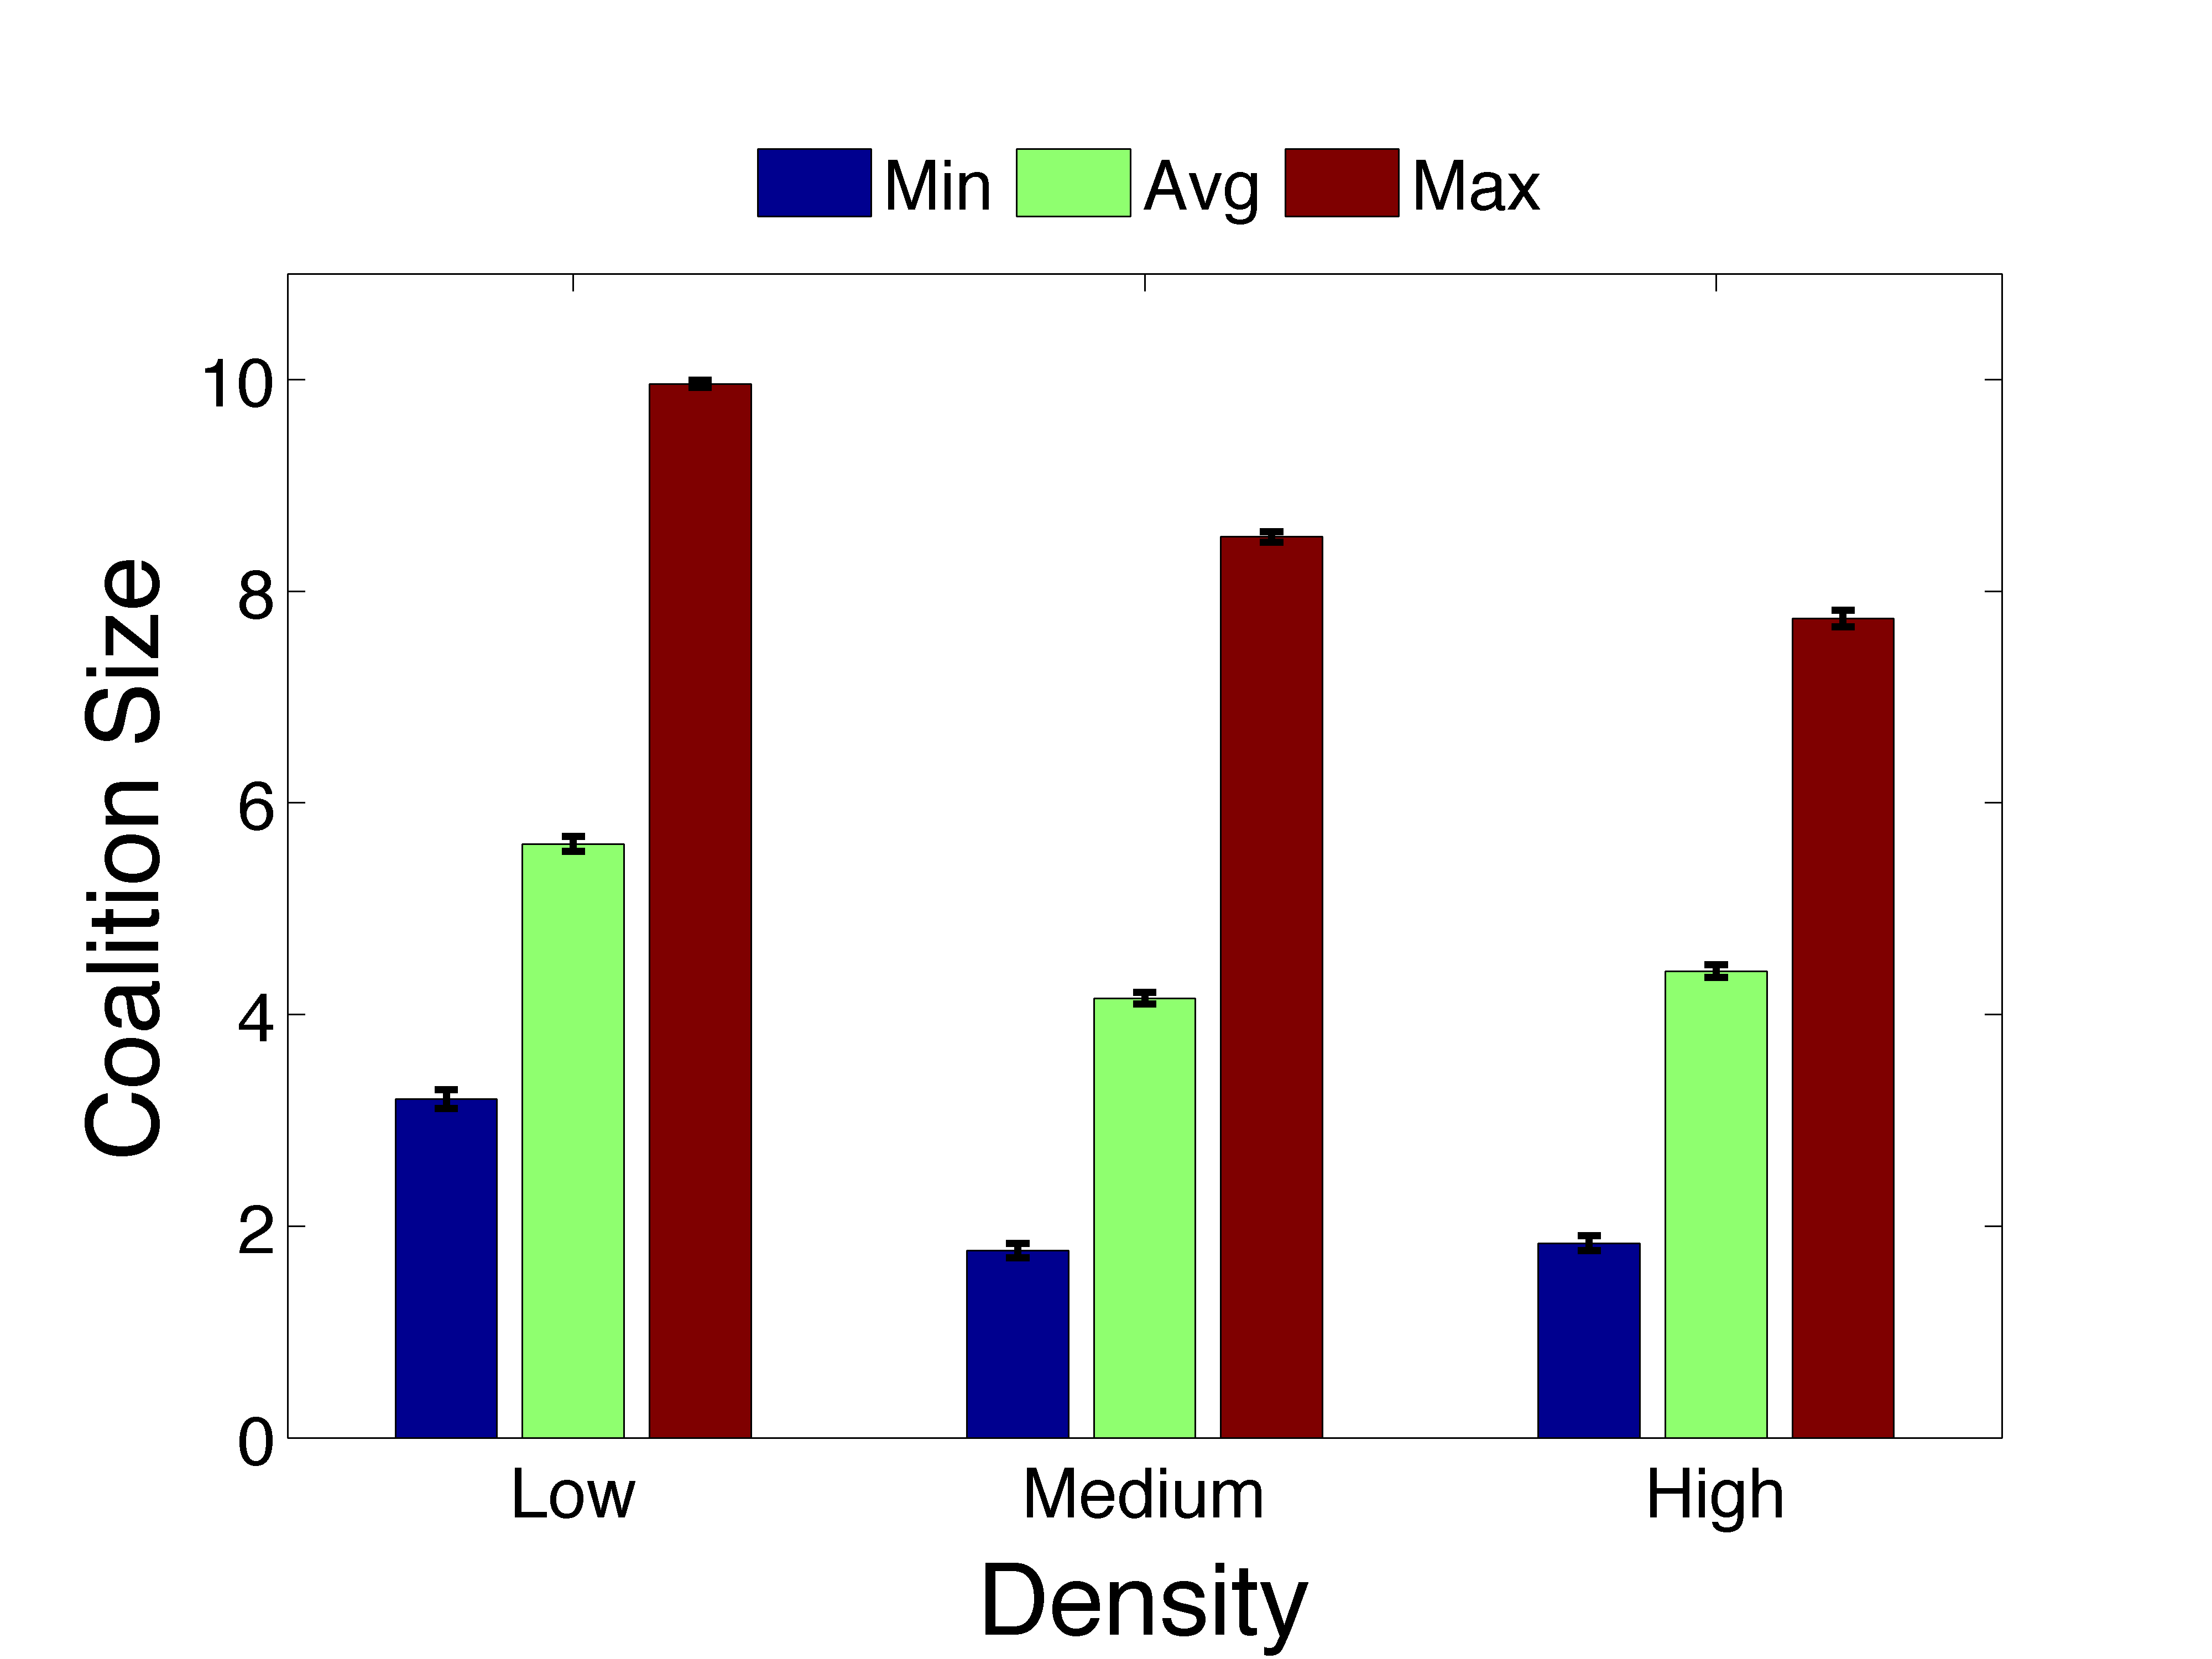
\includegraphics[width=0.49\textwidth,type=png,ext=.png,read=.png]{graphs/ScaleFree-0.875-Size}
	}
	
  \hspace{-0.1in}\subfigure[Small World $M_1$]{
  	%\label{fig:res_mmuca_quality}
	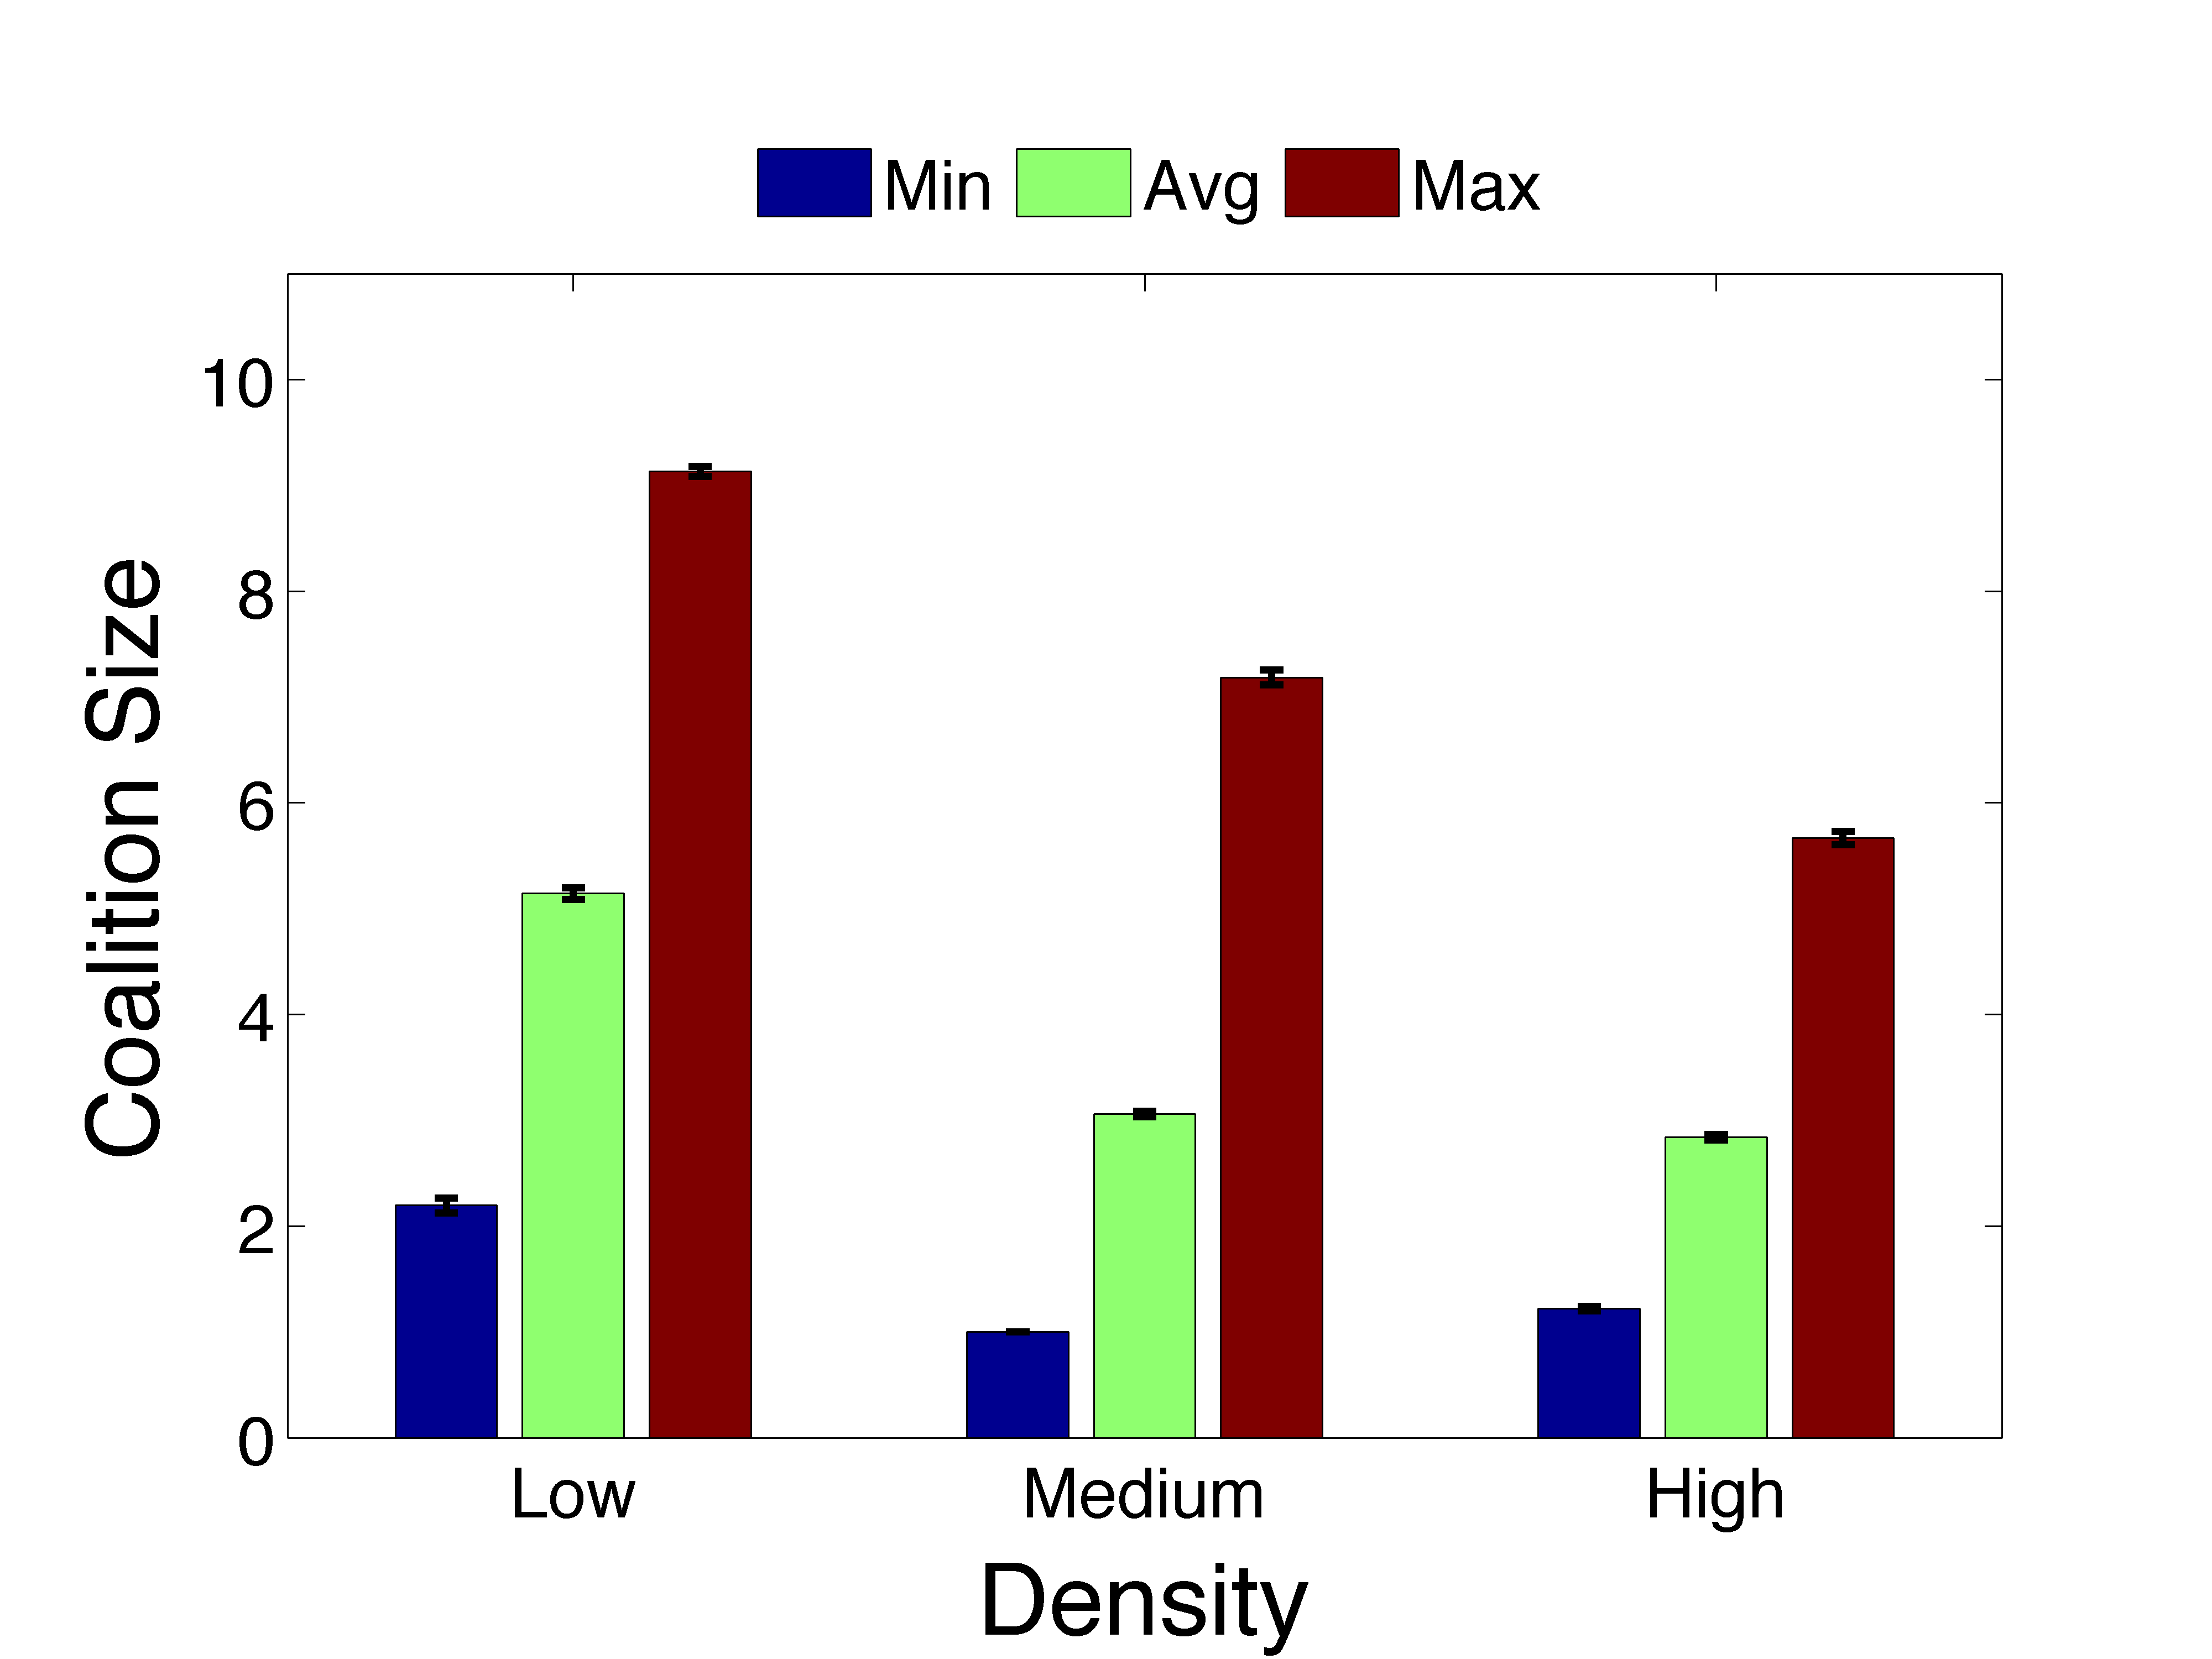
\includegraphics[width=0.49\textwidth,type=png,ext=.png,read=.png]{graphs/SmallWorld-1.000-Size}
	}
  \hspace{-0.1in}\subfigure[Small World $M_2$]{
  	%\label{fig:res_mmuca_quality}
	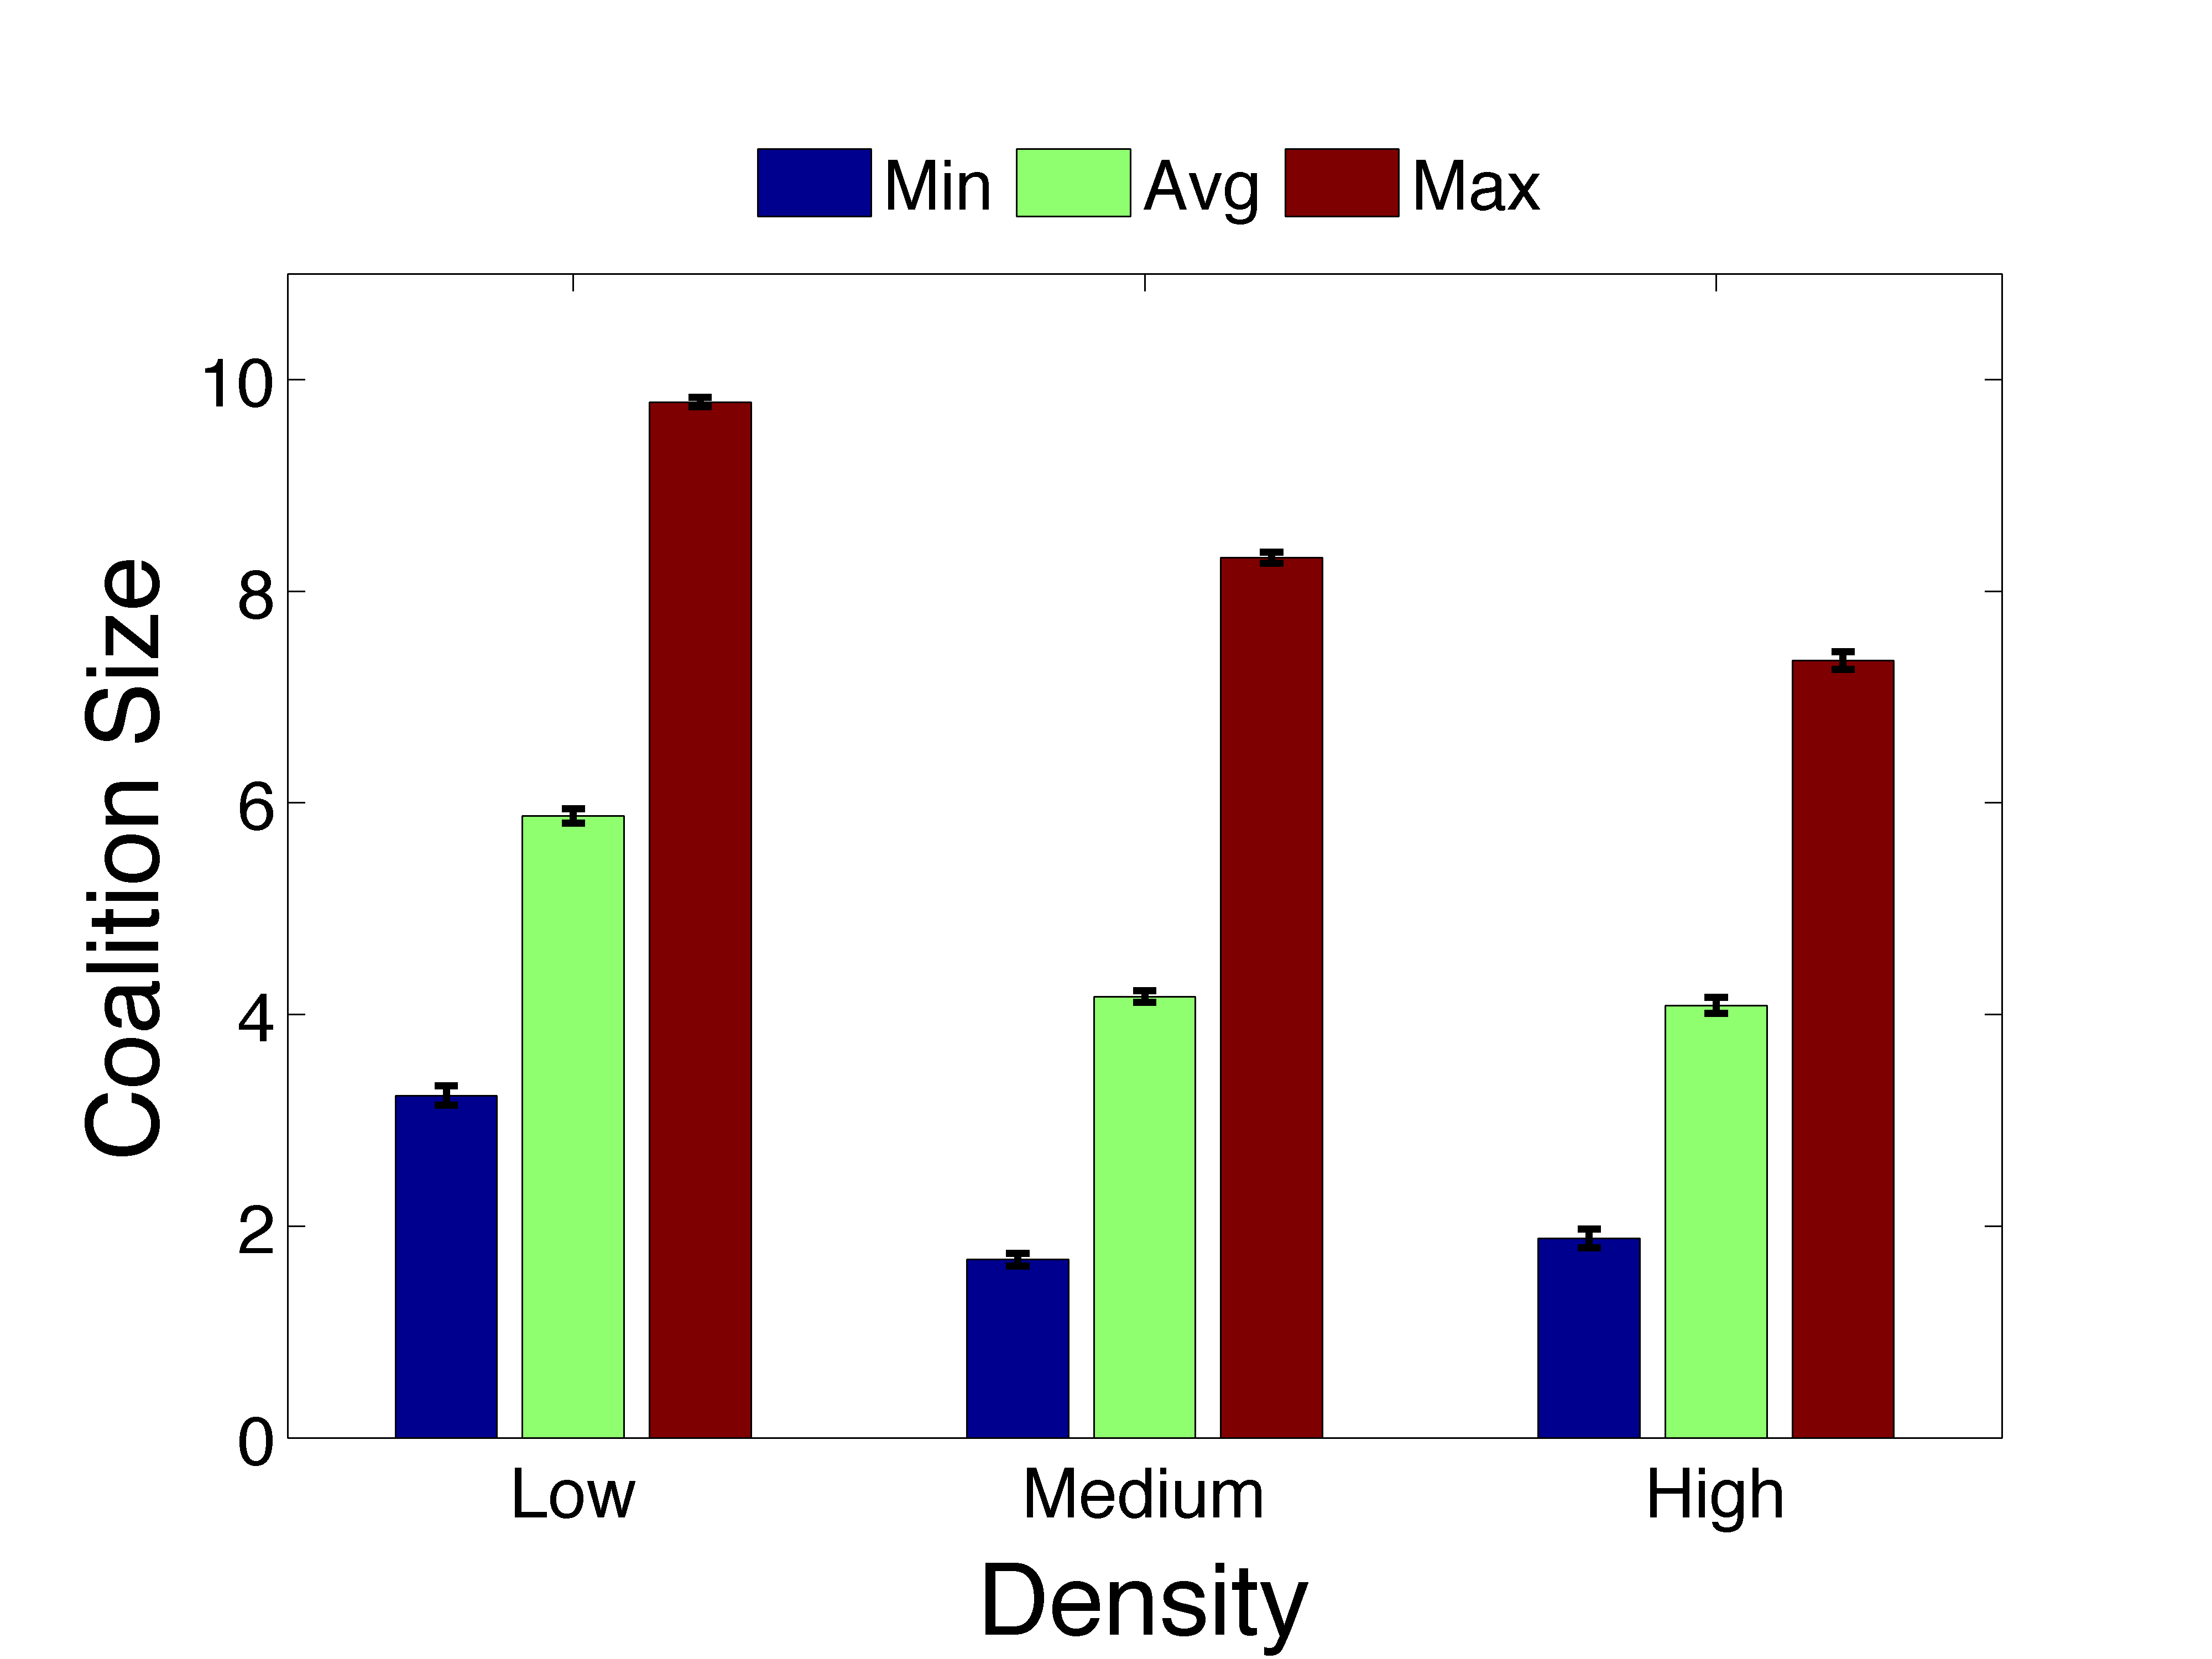
\includegraphics[width=0.49\textwidth,type=png,ext=.png,read=.png]{graphs/SmallWorld-0.875-Size}
	}  
  \caption{Graphs showing the minimum, average and maximum size of
  coalitions formed on different topologies and densities under market conditions $M_1$ (a)-(c), $M_2$
  (d)-(f). }
  \label{fig:graphs_size}
\end{figure*}    

%%%%%%%%%%%%%%%%%%%%%%%%%%%%%%%%%%%%%%%%%%%%%%%%%%%%%%%%%%%%%%%%%%%%%%%%%%%%%%%%%%%%%%%%%%%%%%%%%%%%%%%%%%%%%%%%
%% Chapter %%%%%%%%%%%%%%%%%%%%%%%%%%%%%%%%%%%%%%%%%%%%%%%%%%%%%%%%%%%%%%%%%%%%%%%%%%%%%%%%%%%%%%%%%%%%%%%%%%%%%
%%%%%%%%%%%%%%%%%%%%%%%%%%%%%%%%%%%%%%%%%%%%%%%%%%%%%%%%%%%%%%%%%%%%%%%%%%%%%%%%%%%%%%%%%%%%%%%%%%%%%%%%%%%%%%%%

\chapter{Conclusions and Future Work}\label{chap:concl}

In this thesis we have shown how the stable coalition formation can be effectively applied to a real-world application such the purchase of energy on the wholesale electrical marked. 

Users with complementary consumption profiles can join together in a common group, forming a \textit{coalition} whose aggregate energy demand is more regular and flattened. 
Thus, more of this energy can be retrieved from the long term market, which provides large amounts of energy at a cheaper prices, granting the single agents a real monetary advantage. Also, the request for expensive, carbon-intensive peaking plants generators is reduced, providing a great benefit for the environment.

To help the solving process, the space of research has been reduced by means of a \textit{social network}, which models the social interactions among the users. 
Social networks not only provide a way of connecting
energy consumers but also restrict coalition membership by specifying
realistic constraints to the formation of certain groups. In
particular, consumers may not want to join coalitions with unknown consumers for
which they do not have any source of trust regarding their reported profiles or
their capacity to meet their payment obligations.

The work here presented is very promising and has given good results, as pointed out by the empirical tests. The provided solutions can effectively lower the cost single users have to pay for their electricity bill, with a promising effect from the ecological point of view, due to the limited pollutant emissions.

Moreover, the considered approach is suitable to be applied to real-world scenarios, since it assumes to deal with selfish agents, a typical feature of real energy customers. We remark that the pursuit of \textit{both} optimality and stability has never been covered in literature, while this work addresses the two problematics together.

\noindent Nevertheless, there are many possibilities for future development in this direction. The theoretical representation defined in Chapter \ref{chap:gdl} provides a smart intuition in the context of cooperative games on graphs, but can be further improved to allow a better scalability with respect to the dimension of instances used as inputs for the problem. At the current state, our technique can solve general graphs of 12-13 nodes, with a density of 2.

In addition, the computational complexity of the approach can be lowered (at the expense of the accuracy) adopting approximated or non-complete solving techniques, which may provide a good -- but not optimal -- solution in a reasonable amount of time, even for bigger instances than the ones tractable at the moment.

Focusing on the implementation, a very promising direction of improvement may be represented by the adoption of thread-intensive techniques provided by the GPU computing. Due to the high parallelization characteristics of the routine used in the coalition formation process, the use of a massive multi-threading implementation (such as \textit{CUDA} or \textit{OpenCL}) would grant a great speed-up, though the theoretical computational complexity would not be affected.

Finally, the metrics proposed in Section \ref{sec:metric} (especially the \textit{user price factor}) have proven to be effective in the tests, but alternative forms of evaluation of the coalitions are not to be excluded, for example considering features other than the simple price paid by the customers or managing the risks with different approaches.

In conclusion, the work of this thesis has given a great contribution in the field of stable coalition formation theory, especially considering the approach of new and interesting problematics in the energetic domain and providing a novel and brilliant solving technique, which may be the starting point of many future developments.

\bibliographystyle{splncs03}
\bibliography{thesis}

\end{document}
